%%%%%%%%%%%%%%%%%%%%%%%%%%%%%%%%%%%%%%%%%%%%%%%%%%%%%%%%%%%%%%%%%
% Tese de Doutorado / Dept Fisica, CFM, UFSC                    %
% Andre@UFSC - 2014                                             %
%%%%%%%%%%%%%%%%%%%%%%%%%%%%%%%%%%%%%%%%%%%%%%%%%%%%%%%%%%%%%%%%%
\documentclass[final]{nathesis_A5}

\begin{document}

\frontmatter
  \pagenumbering{arabic}
  %%%%%%%%%%%%%%%%%%%%%%%%%%%%%%%%%%%%%%%%%%%%%%%%%%%%%%%%%%%%%%%%%
% Tese de Doutorado / Dept Fisica, CFM, UFSC                    %
% André@UFSC - 2015                                             %
%%%%%%%%%%%%%%%%%%%%%%%%%%%%%%%%%%%%%%%%%%%%%%%%%%%%%%%%%%%%%%%%%


%***************************************************************%
%                                                               %
%               Capa (Na verdade, folha de rosto)               %
%                                                               %
%***************************************************************%
\label{rosto}
\pdfbookmark[0]{Folha de rosto}{rosto}

\institution{Universidade Federal de Santa Catarina \\
        Centro de Ciências Físicas e Matemáticas \\
        Curso de Pós-Graduação em Física}

\thesistitle{Espectroscopia 3-D de galáxias:\\
síntese de populações estelares e morfologia}

\thesisauthor{André Luiz de Amorim}

\supervisor{Orientadores: \\
        Dr.\ Roberto Cid Fernandes Jr. (UFSC) \\ 
        Dra.\ Rosa María González Delgado (IAA)}

\comments{Tese submetida ao Programa de Pós-Graduação em Física da Universidade
Federal de Santa Catarina para a obtenção do título de Doutor em Física.
Trabalho financiado por CNPq e CAPES.}

\place{Florianópolis}

\thesisdate{2015}

\titlepage

% End of this chapter

  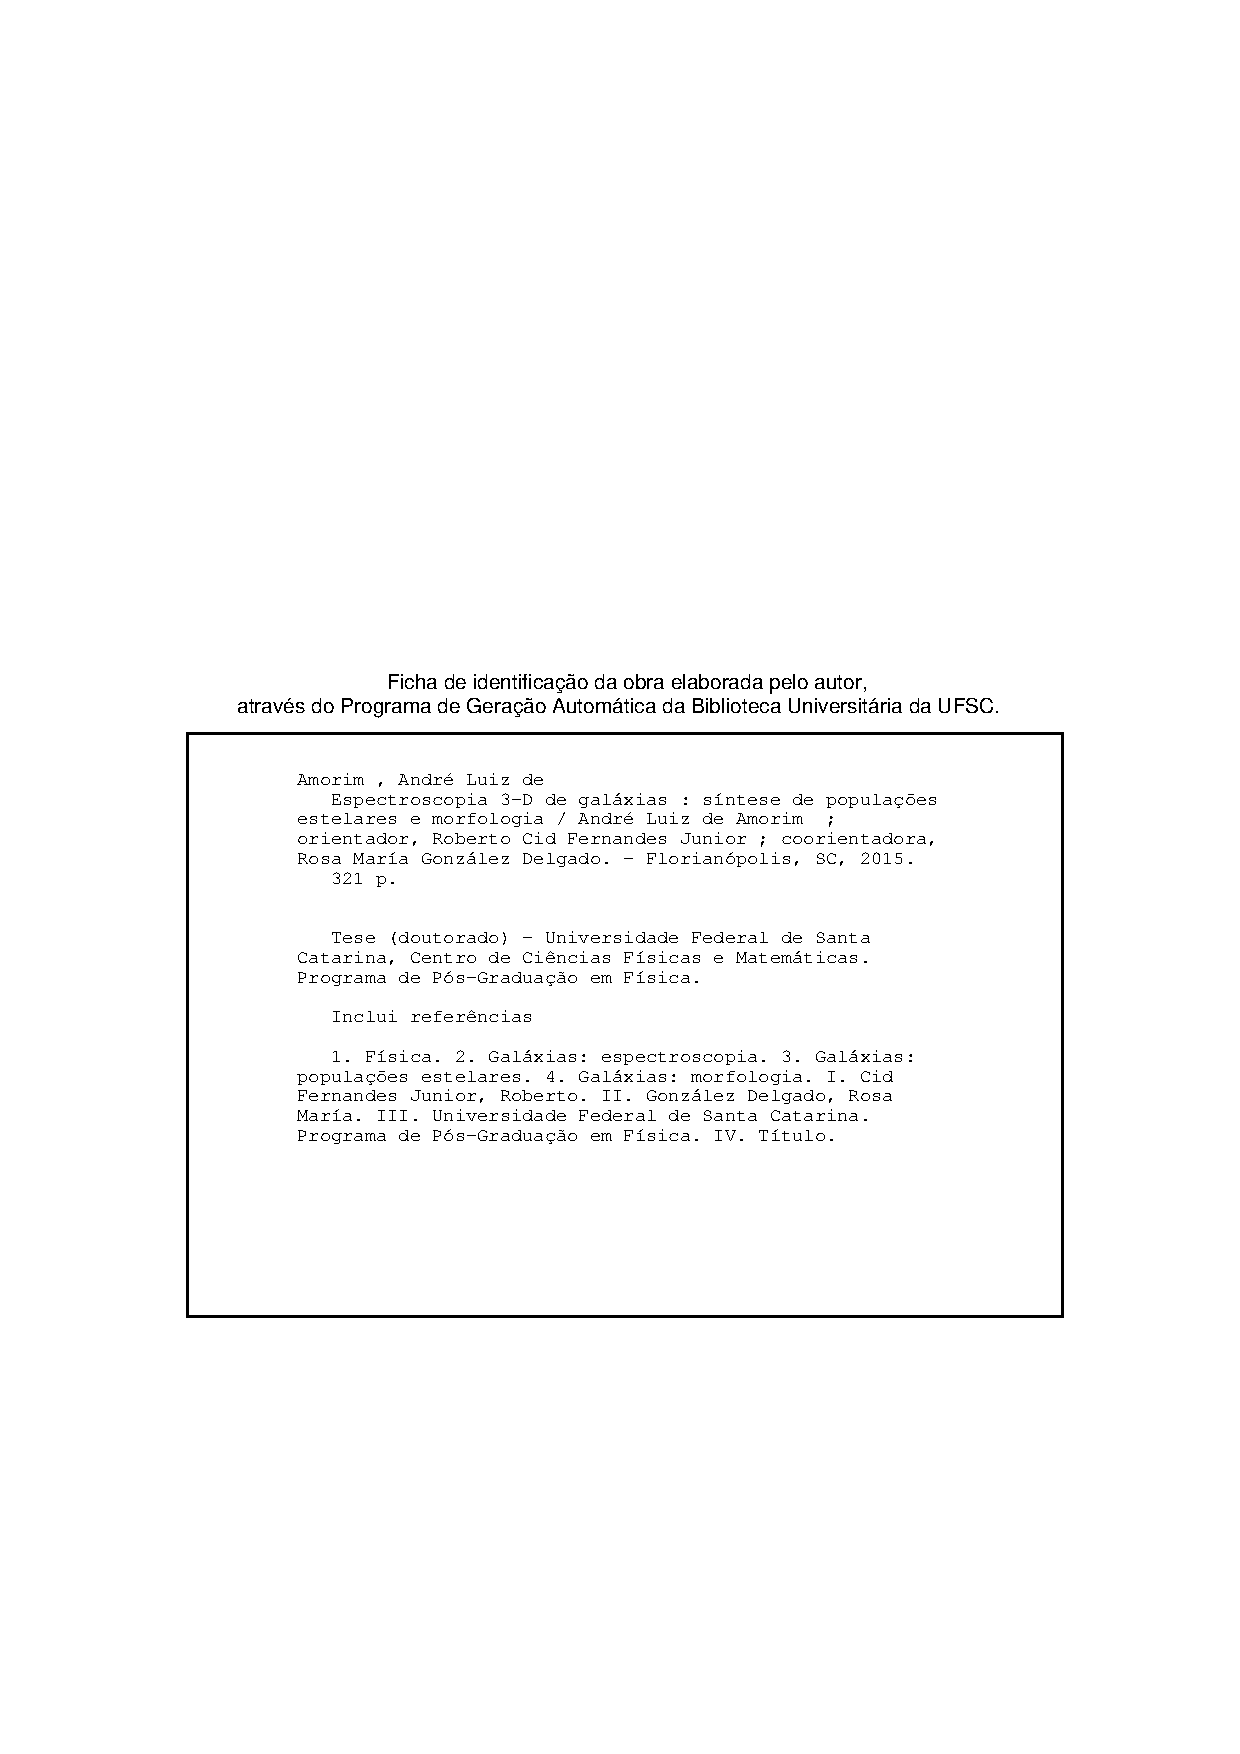
\includepdf[pages=1]{bib_ufsc/ficha_catalografica.pdf}
  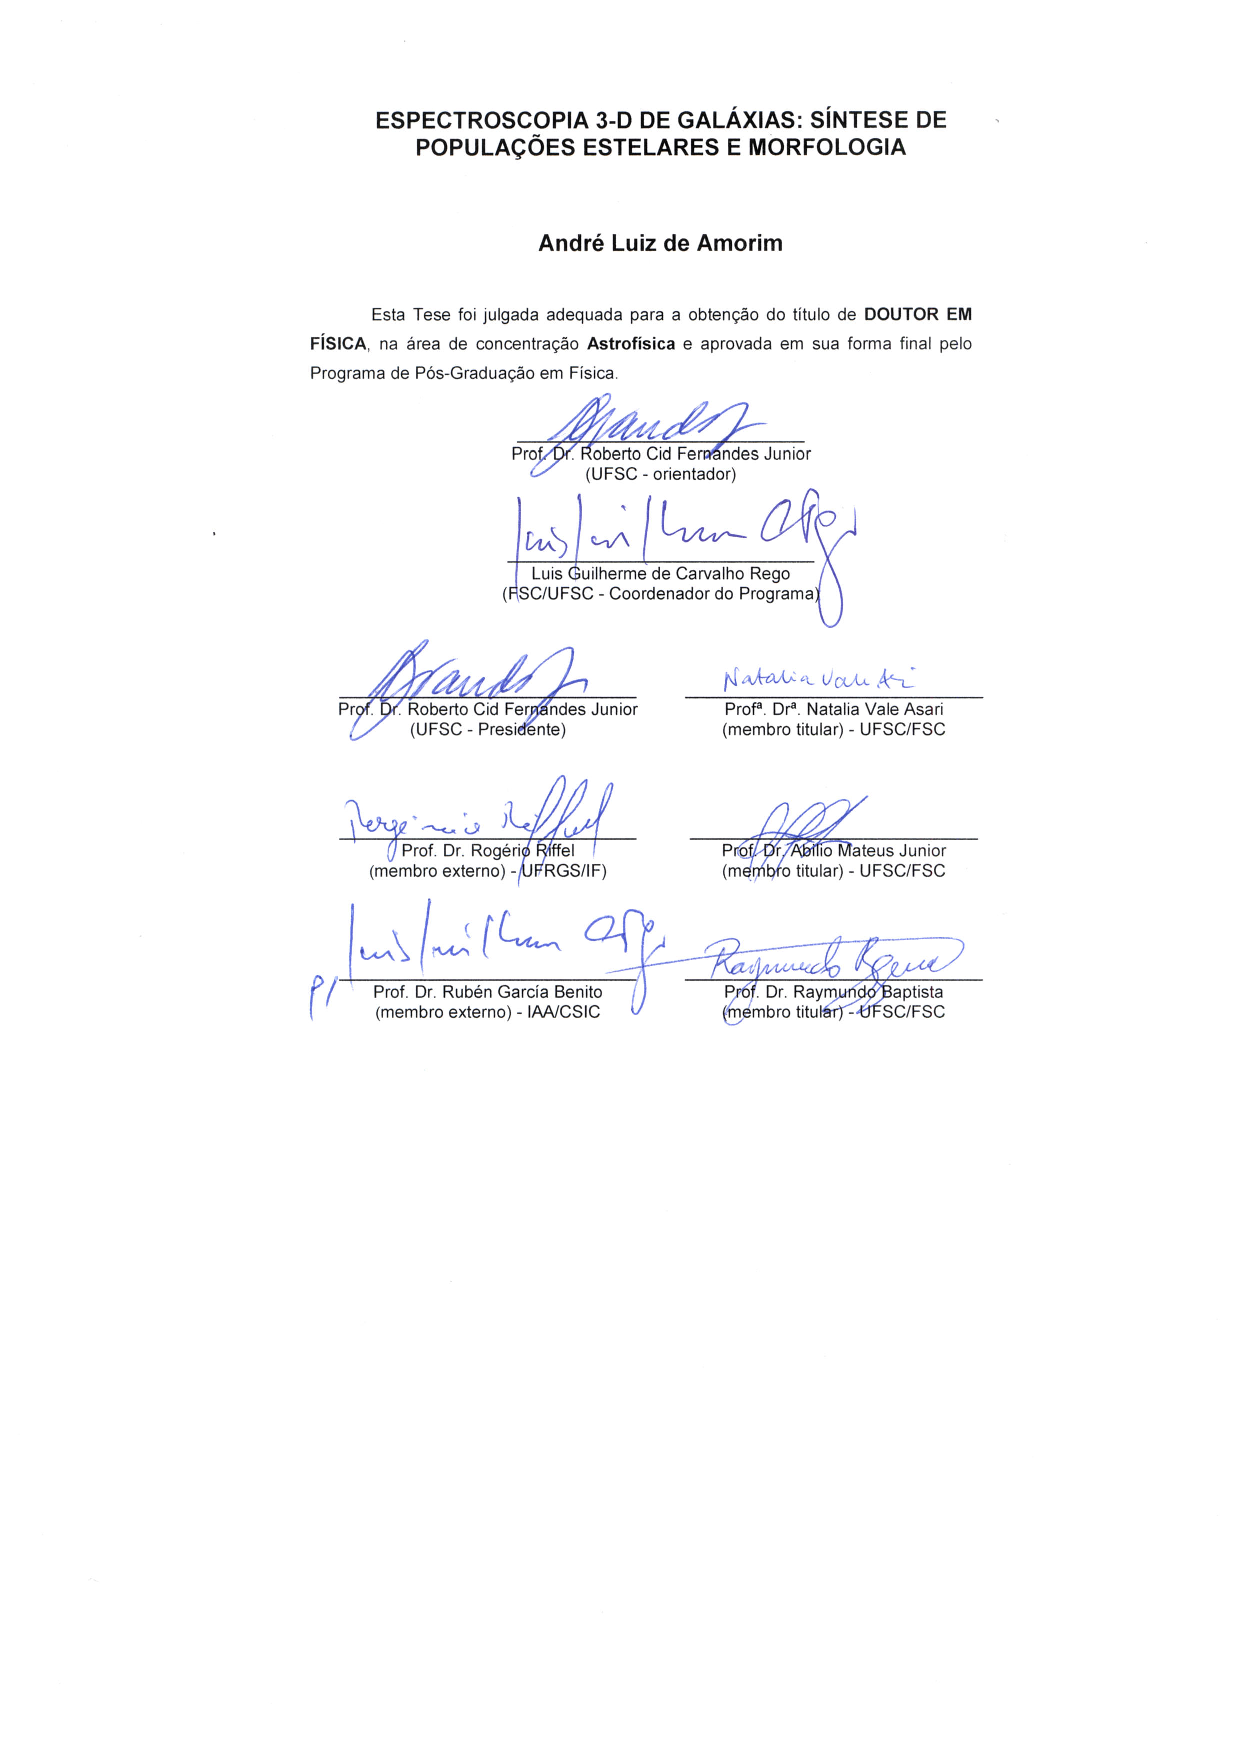
\includepdf[pages=1,trim=31mm 87mm 31mm 0mm,clip]{bib_ufsc/banca.pdf}\cleardoublepage

  %%%%%%%%%%%%%%%%%%%%%%%%%%%%%%%%%%%%%%%%%%%%%%%%%%%%%%%%%%%%%%%%%
% Dissertacao de Mestrado / Dept Fisica, CFM, UFSC              %
% Andre@UFSC - 2011                                             %
%%%%%%%%%%%%%%%%%%%%%%%%%%%%%%%%%%%%%%%%%%%%%%%%%%%%%%%%%%%%%%%%%


%***************************************************************%
%                                                               %
%                          Dedicatória                          %
%                                                               %
%***************************************************************%

\thispagestyle{plain}

\

\vfill

\begin{flushright}
\hfill \textit{A meus pais e avós.}
\end{flushright}

\vspace*{1cm}

\clearpage

  %%%%%%%%%%%%%%%%%%%%%%%%%%%%%%%%%%%%%%%%%%%%%%%%%%%%%%%%%%%%%%%%%
% Dissertacao de Mestrado / Dept Fisica, CFM, UFSC              %
% Andre@UFSC - 2011                                             %
%%%%%%%%%%%%%%%%%%%%%%%%%%%%%%%%%%%%%%%%%%%%%%%%%%%%%%%%%%%%%%%%%


%***************************************************************%
%                                                               %
%                        Agradecimentos                         %
%                                                               %
%***************************************************************%

\chapter*{Agradecimentos}

Agradeço primeiro à minha esposa Marilize, que tanto me apoiou nesta aventura, e
com quem terei junto a maior aventura de todas, que vai chegar logo, logo. 
Agradeço também aos meus pais e irmãos pelo amor e companheirismo, e por eu
sempre poder contar com eles.

Ao meu orientado e grande amigo Cid, por todas as oportunidades, e pelas
infindáveis discussões, às vezes sobre esta tese, e muitas vezes muito bem
regadas. À Rosa, minha orientadora no IAA, que nos recebeu, eu e Marilize, com
tanto carinho tão longe de casa. E principalmente por dar um norte científico a
alguém que costumava pensar primeiro nos aspectos técnicos do trabalho.

Também ao Enrique, à Natalia e ao Rubén, sempre com ideias geniais, muitas das
quais encontrando o seu caminho para esta tese. Se há resultados bons nestes
trabalho, seus conselhos, dicas e sugestões tiveram um papel fundamental.

Aos colegas de estudos, William, Eduardo, Fábio, Rafa, Clara e todo o pessoal
do Grupo de Astrofísica e do IAA, pelo ambiente agradável de trabalho; muitas
amizades que devo levar pro resto da vida.

Este trabalho não seria possível sem os recursos financeiros da Coordenação de
Aperfeiçoamento de Pessoal do Nível Superior, CAPES; do Conselho Nacional de
Desenvolvimento Científico e Tecnológico, CNPq; do Instituto Nacional de Ciência
e Tecnologia de Astrofísica, INCT-A; do programa Ciência sem Fronteiras; e do
Instituto de Astrofísica de Andalucía, IAA/CSIC. Também sou grato ao Curso de
Pós Graduação em Física, tanto pelo apoio financeiro quanto pela estrutura e
instalações adequadas.

Finalmente, agradeço à colaboração do CALIFA, pelas inúmeras discussões e
sugestões, especialmente nas {\em Busy Weeks}, sempre produtivas. E
principalmente à equipe de observação e redução por produzir os dados com tanto
capricho e dedicação, fundações sobre as quais este trabalho se ergueu.

% End of Acknowledgments

  %%%%%%%%%%%%%%%%%%%%%%%%%%%%%%%%%%%%%%%%%%%%%%%%%%%%%%%%%%%%%%%%%
% Dissertacao de Mestrado / Dept Fisica, CFM, UFSC              %
% Andre@UFSC - 2011                                             %
%%%%%%%%%%%%%%%%%%%%%%%%%%%%%%%%%%%%%%%%%%%%%%%%%%%%%%%%%%%%%%%%%

%***************************************************************%
%                                                               %
%                          Resumo                               %
%                                                               %
%***************************************************************%

\begin{abstract}[Resumo]

Neste trabalho foram desenvolvidas ferramentas para trabalhar com espectros de
campo integral (IFS) do {\em survey} CALIFA. Os espectros dos {\em spaxels} são
preprocessados e em seguida analisados com o uso do programa \starlight. Uma das
ferramentas principais discutidas aqui, PyCASSO, organiza os arquivos de saída
do \starlight em cubos de dados de produtos da síntese de população estelar. Ele
também permite uma programação interativa e exploratória, dando acesso de forma
prática e simples aos dados multidimensionais.

Através do uso destas ferramentas, foi desenvolvido um método que obtém e
analisa as populações estelares das componentes morfológicas (bojo e disco) de
galáxias, a partir de dados de IFS. A decomposição morfológica é feita
utilizando o programa IMFIT, com um {\em wrapper} em Python. Uma amostra de 43
galáxias classificadas com S0 e com baixa inclinação foi escolhida para
aplicação do método. O modelo morfológico utilizado foi um bojo com perfil de
Sérsic e um disco exponencial. A decomposição morfológica é feita a cada
comprimento de onda, de tal forma que se obtém ao final um espectro para cada
{\em pixel} do bojo e do disco. Uma boa medida da PSF é essencial neste
procedimento, então foi feita a caracterização da PSF do CALIFA utilizando as
estrelas de calibração do {\em survey}. Os parâmetros morfológicos ($r_e$, $n$,
P.A. e $\epsilon$ para o bojo, $h$, P.A. e $\epsilon$ para o disco), na maioria
dos casos, depende linearmente, em média, do comprimento de onda, mas o seu
comportamento a cada $\lambda$ ainda não é bem compreendido. Foi feita a síntese
espectral de populações estelares das componentes morfológicas de 9 galáxias da
amostra, que tiveram um bom resultado na decomposição. Apenas duas destas
produziram bons ajustes com o \starlight, CALIFA 0592 (NGC 4874) e CALIFA 0858
(UGC 10905). Em ambos os casos se obtém um bojo mais velho e menos metálico e um
disco mais jovem e mais metálico do que o resultado da síntese do espectro
observado. A síntese de populações estelares utilizando os espectros integrados
produziram resultados mais robustos. Os espectros espacialmente resolvidos do
bojo e do disco parecem ter artefatos que interferem no ajuste do \starlight,
sendo interpretados como poeira, entre outras coisas, levando a resultados
equivocados.

\clearpage

% Ou\ldots
% 
% a figura a seguir resume esta tese.
% 
% \begin{center}
% 
\includegraphics[width=0.7\textwidth]{figuras/lmp}
% \end{center}

\end{abstract}

% End of resumo

  %%%%%%%%%%%%%%%%%%%%%%%%%%%%%%%%%%%%%%%%%%%%%%%%%%%%%%%%%%%%%%%%%
% Dissertacao de Mestrado / Dept Fisica, CFM, UFSC              %
% Andre@UFSC - 2011                                             %
%%%%%%%%%%%%%%%%%%%%%%%%%%%%%%%%%%%%%%%%%%%%%%%%%%%%%%%%%%%%%%%%%

%***************************************************************%
%                                                               %
%                          Abstract                             %
%                                                               %
%***************************************************************%

\begin{abstract}

We developed a method for recovering and analysing the stellar populations of
the different morphological components of galaxies using integral spectroscopy
data. Using the software Imfit, wrapped in Python, we perform the decomposition
of a sample of 53 candidate S0 galaxies from the CALIFA Survey into a Sérsic
bulge and an exponential disk. The decomposition is made wavelength-wise, so
that at the end we get the bulge and disk spectra for each pixel. The
morphological parameters ($R_e$, $n$, P.A. and $\epsilon$ for bulge, $h$, P.A.
and $\epsilon$ for disk) in most cases depends linearly on the wavelength, at
least for wavelengths $> 4000\,\angstrom$. Using the decomposed spectra from two
galaxies from the sample (NGC 1375 and NGC 7194), we apply a stellar population
synthesis using STARLIGHT, in order to recover the stellar populations of bulge
and disk. In both cases we recover an old bulge and an intermediate aged disk.
We also obtain a weak but positive stellar age gradient for the bulges and no
measurable gradient for the disks.


\end{abstract}

% End of abstract




  
  \tableofcontents\clearpage
  \listoffigures\clearpage
  \listoftables\clearpage

\mainmatter*

  % Introdução
  %%%%%%%%%%%%%%%%%%%%%%%%%%%%%%%%%%%%%%%%%%%%%%%%%%%%%%%%%%%%%%%%%
% Tese de Doutorado / Dept Fisica, CFM, UFSC                    %
% Andre@UFSC - 2014                                             %
%%%%%%%%%%%%%%%%%%%%%%%%%%%%%%%%%%%%%%%%%%%%%%%%%%%%%%%%%%%%%%%%%

%:::::::::::::::::::::::::::::::::::::::::::::::::::::::::::::::%
%                                                               %
%                          Capítulo 1                           %
%                                                               %
%:::::::::::::::::::::::::::::::::::::::::::::::::::::::::::::::%

%***************************************************************%
%                                                               %
%                         Introdução                            %
%                                                               %
%***************************************************************%

\chapter{Introdução}
\label{sec:intro}

%***************************************************************%
%                                                               %
%                         Intro - IFS                           %
%                                                               %
%***************************************************************%

\section{Espectroscopia de campo integral}

Na última década presenciamos uma proliferação de surveys de imageamento e
espectroscopia. Surveys como o SDSS \citep{York2000}, ALHAMBRA \citep{Moles2008}
e COSMOS \citep{Scoville2007}, para citar alguns exemplos, permitem explorar a
distribuição espectral de energia (SED\footnote{\em Spectral Energy
Distribution.}) de centenas de milhares a milhões de galáxias.
Entretanto, da forma como estes surveys são executados, há sempre um compromisso
entre a resolução espacial e a espectral. As imagens obtidas pelo SDSS têm um
boa resolução espacial, mas mapeiam a SED de forma grosseira, com apenas $5$
filtros de banda larga ($ugriz$). Já os espectros obtidos pelo mesmo survey
possuem uma excelente resolução e cobertura espectral, mas obtém o espectro
integrado da região central das galáxias.

O melhor dos dois mundos pode ser alcançado com instrumentos que fazem
espectroscopia de campo integral (IFS\footnote{\em Integral Field
Spectroscopy.}). Instrumentos que realizam este tipo de espectroscopia consistem
em geral de um amontoado de fibras óticas, as quais alimentam um espectrógrafo
comum. Assim, depois de um processo relativamente complicado de redução de
dados, obtém-se espectros espacialmente resolvidos com uma boa resolução
espectral e espacial. O survey CALIFA ({\em Calar Alto Legacy Integral Field
Area survey\footnote{\url{http://www.caha.es/CALIFA/}}}) está utilizando o
instrumento PMAS/PPAK do observatório Calar Alto para obter IFS de $600$
galáxias \citep{Sanchez2012}.
Destas, $100$ já estão disponíveis no primeiro {\em Data Release}
\citep[DR1]{Husemann2013}, afirmando o caráter de legado deste
survey.\fixme(atualizar comentário sobre data releases)

Quando completado, o CALIFA terá obtido da ordem de $10^6$ espectros, quase o
mesmo que o SDSS. Porém, este não será apenas mais um survey espectroscópico. A
riqueza do CALIFA está nas informações espacialmente resolvidas, em uma amostra
representativa do universo local ($0.005 < z < 0.03$, limitada em diâmetro
angular) cobrindo a distribuição de galáxias no diagrama cor--magnitude da nuvem
azul à sequência vermelha, amostrando galáxias todos os tipos morfológicos
(espirais, elípticas, irregulares e até mesmo alguns sistemas em interação).

\begin{figure}
	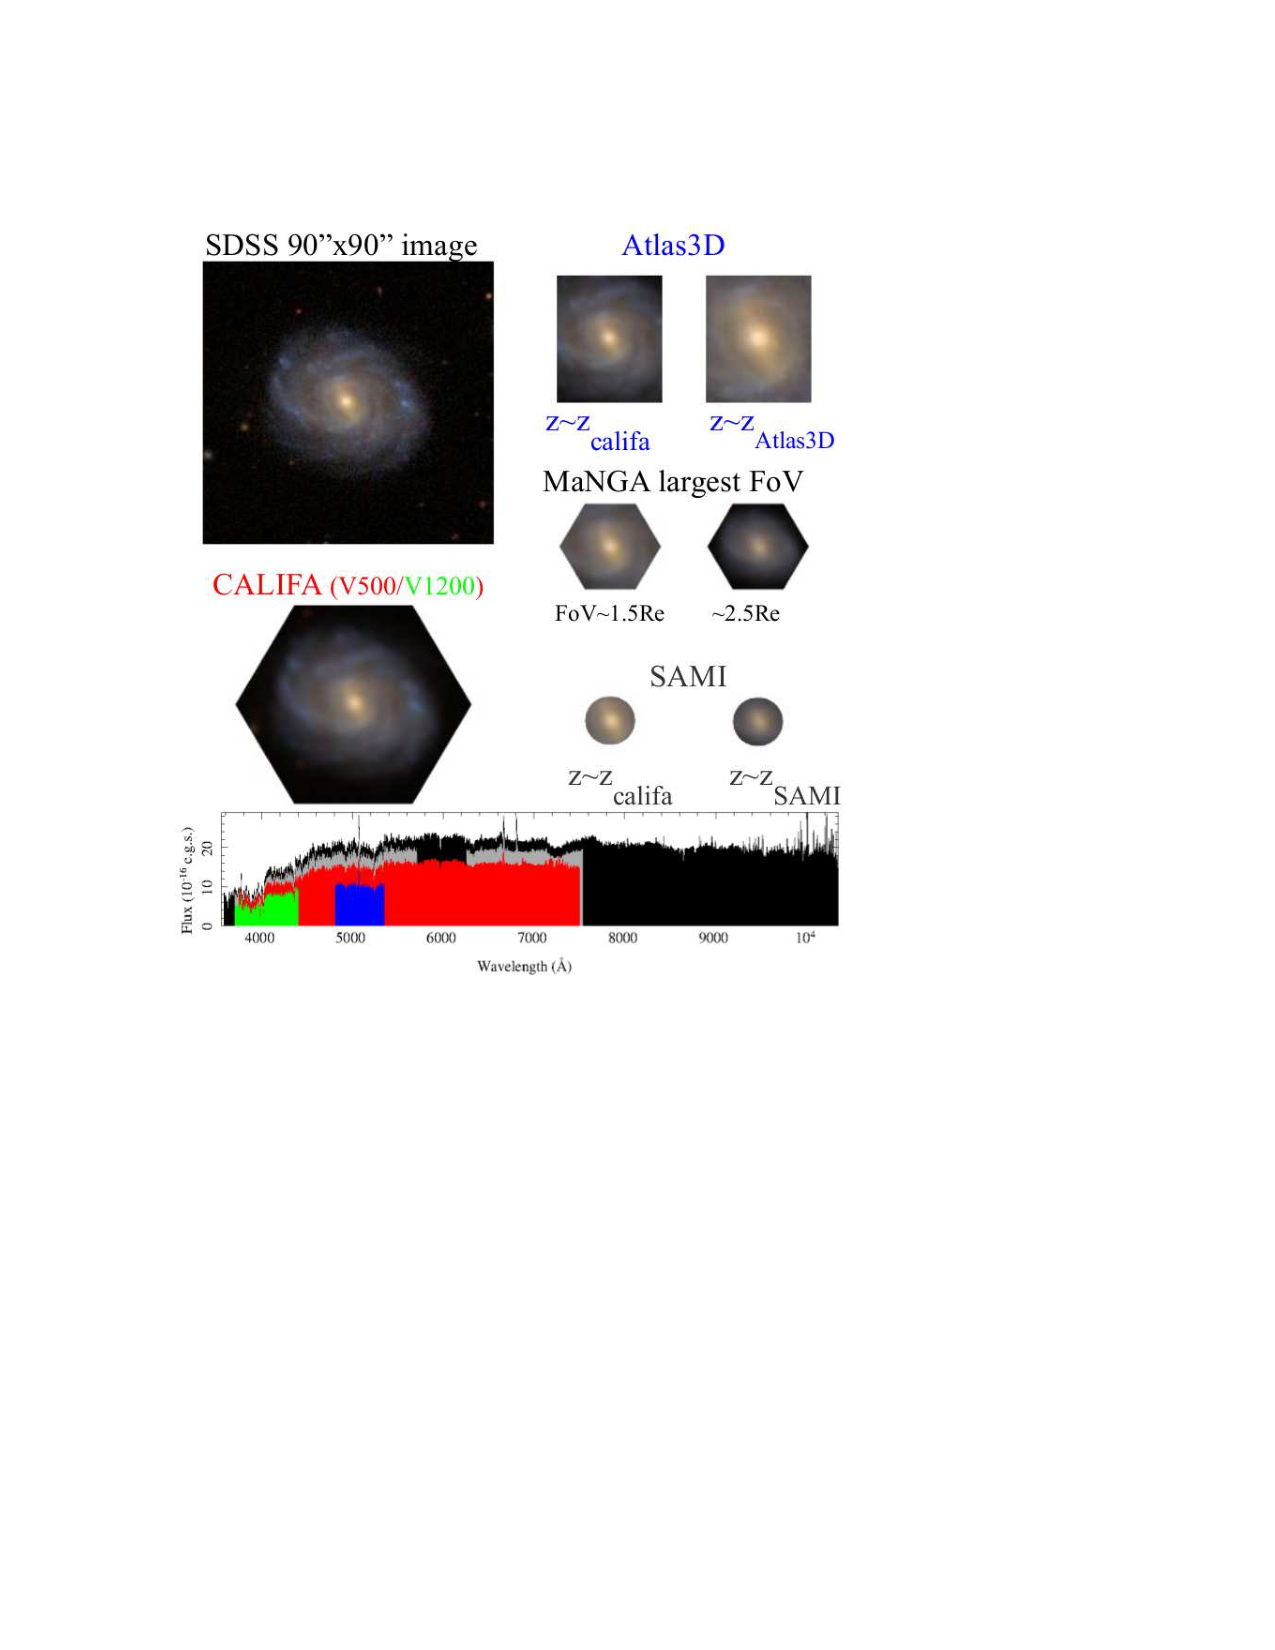
\includegraphics{figuras/surveysIFS}
	\caption[Comparação entre {\em surveys} espectroscópicos de campo integral.]
	{\TODO: Comparação entre {\em surveys} espectroscópicos de campo integral.
	Retirado de \citet{Sanchez2014}.}
	\label{fig:surveysIFS}
\end{figure}

Comparado a outros {\em surveys} já realizados, como o Altas3D
\citep{Cappellari2011} ou o {\em Disk Mass Survey} (DMS) \citep{Bershady2010}, o
CALIFA cobre uma faixa muito maior de tipos morfológicos e massas. Outros {\em
surveys} que estão em andamento são o SAMI \citep{Croom2012, Bryant2015} e o
MaNGA \citep{Bundy2015}. Estes também buscam obter uma amostra grande de
galáxias, até maior do que a do CALIFA. Entretanto, a vantagem do CALIFA está na
cobertura e amostragem espacial, observando uma maior porção de cada galáxia com
mais riqueza de detalhes. \TODO Falar da Figura \ref{fig:surveysIFS}, pegar
alguma coisa de \citet{Sanchez2014}.

%***************************************************************%
%                                                               %
%                Intro - Stellar synthesis of IFS               %
%                                                               %
%***************************************************************%

\section{Síntese de população estelar espacialmente resolvida}
\label{sec:Intro:Sintese}

Os espectros espacialmente resolvidos do CALIFA podem ser descritos como um cubo
de dados, com as duas primeiras dimensões sendo a posição $x$ e $y$ (ascensão
reta e declinação) e a terceira sendo o comprimento de onda. Nestes cubos,
planos com comprimento de onda constante são imagens, enquanto ``fatias''
definidas por um par $(x, y)$ constante são espectros. Pode-se tratar estes
espectros individualmente, embora na verdade, nos cubos do CALIFA os pixels
vizinhos estão correlacionados devido ao {\em seeing} do céu e ao processo de
observação. Há a queda na relação sinal/ruído (S/N) nas regiões mais afastadas
do núcleo da galáxia, onde o brilho superficial é muito menor.
Algumas galáxias possuem outros objetos ``intrusos'' que precisam ser
mascarados. Linhas telúricas\footnote{Linhas de absorção causadas pela
atmosfera.} também precisam ser mascaradas. Assim, em geral, é necessário um
preprocessamento visando manter um S/N mínimo e garantir um espectro livre de
contaminação. Os detalhes sobre o preprocessamento utilizado neste trabalho
estão descritos na seção 3 do Apêndice \ref{apendice:PaperResolving1}.

Um aspecto importante do preprocessamento utilizado é que o cubo de dados é
dividido em zonas de Voronoi, onde regiões com baixo S/N são combinadas formando
efetivamente ``pixels maiores''. Desta forma, o cubo original é transformado
numa matriz de zonas e comprimento de onda, onde fatias de zona constante são
espectros. Com isso, os espectros, e as máscaras e erros que os acompanham,
estão prontos para serem usados pelo próximo passo.

A síntese de população estelar consiste em obter a história de formação estelar
(SFH) de uma galáxia utilizando modelos de população estelar simples (SSP).
Ajusta-se o espectro de uma galáxia como a soma de espectros de SSPs com idades
e composições químicas distintas (levando em conta a atenuação por poeira). O
resultado é um vetor de frações de luz e massa destas SSPs, que podem ser
facilmente convertidos a uma SFH conforme a prescrição de \cite{Asari2007}.
O programa utilizado é o \starlight, desenvolvido por \cite{CidFernandes2005}.

Passamos todos os espectros das zonas pelo \starlight, obtendo o resultado da
síntese como um arquivo de síntese separado para cada zona. Entretanto, para
visualizar ou mesmo tentar entender estes resultados, é preciso organizar e
converter estes arquivos para um formato mais adequado.


%***************************************************************%
%                                                               %
%                        Intro - PyCASSO                        %
%                                                               %
%***************************************************************%

\section{O nascimento do PyCASSO}

Todo o descrito anteriormente forma o alicerce deste presente trabalho. Porém,
dada a grande quantidade de dados espalhados em diversos formatos, a análise dos
resultados da síntese de populações estelares para uma determinada galáxia pode
se tornar um grande e complexo quebra-cabeças computacional. Trabalhar com todas
as galáxias do {\em survey} fica virtualmente impossível desta forma. Assim, da
necessidade de manipular os resultados da síntese dos cubos de dados das
galáxias do CALIFA, nasceu o software PyCASSO.

PyCASSO ({\em Python CALIFA \starlight Synthesis Organizer}) é um software
desenvolvido em Python com o objetivo de organizar gerenciar os dados produzidos
pelo \starlight com base nos dados do CALIFA. O survey CALIFA é apresentado no
Capítulo \ref{sec:ifs}, que também discute os softwares QBICK e \starlight,
ferramentas básicas em nossa análise doe cubos de dados. O Capítulo
\ref{sec:pycasso} apresenta a documentação do PyCASSO, e em seguida discute os
artigos publicados que o utilizam intensivamente.


%***************************************************************%
%                                                               %
%                      Intro - Decomposicao                     %
%                                                               %
%***************************************************************%

\section{Decomposição morfológica de galáxias}

\TODO detalhar mais aqui, ainda não tá legal. O Capitulo \ref{sec:morph}
apresenta um beabá sobre morfologia.

\TODO Caracterização ds PSF no Capítulo \ref{sec:psf}. Explicar a importância
de fazer isso pro survey.

Como aplicação científica do PyCASSO, o Capítulo \ref{sec:pop} trata da síntese
espectral das componentes morfológicas (bojo e disco) de uma galáxia, obtidas no
conforme foi descrito no Capítulo \ref{sec:Decomp}. Estas componentes são
armazenadas em cubos de dados, e são tratados exatamente da mesma forma que
uma galáxia. Seus espectros são passados pelo \starlight, resultando em cubos
de síntese espectral. Os dados da síntese das componentes foram comparados com a
síntese da galáxia original, utilizando o programa PyCASSO. \TODO O que
resultou?


% End of this chapter

  
  % IFS + CALIFA
  %%%%%%%%%%%%%%%%%%%%%%%%%%%%%%%%%%%%%%%%%%%%%%%%%%%%%%%%%%%%%%%%%
% Tese de Doutorado / Dept Fisica, CFM, UFSC                    %
% Andre@UFSC - 2014                                             %
%%%%%%%%%%%%%%%%%%%%%%%%%%%%%%%%%%%%%%%%%%%%%%%%%%%%%%%%%%%%%%%%%

%:::::::::::::::::::::::::::::::::::::::::::::::::::::::::::::::%
%                                                               %
%                          Capítulo 2                           %
%                                                               %
%:::::::::::::::::::::::::::::::::::::::::::::::::::::::::::::::%

%***************************************************************%
%                                                               %
%                         IFS + CALIFA                          %
%                                                               %
%***************************************************************%

\chapter{Síntese de populações estelares em espectroscopia de campo integral}
\label{sec:ifs}

%***************************************************************%
%                                                               %
%                         Section 1                             %
%                                                               %
%***************************************************************%

\section{O {\em survey} CALIFA}

O {\em Centro Astronómico Hispano Alemán} (CAHA) se localiza na {\em Sierra de
los Filabres}, na Comunidade Autônoma de Andaluzia, Espanha. Ele é operado pelo
{\em Max-Planck-Institut für Astronomie} (MPIA), em Heidelberg, Alemanha, e pelo
{\em Instituto de Astrofísica de Andalucía} (IAA/CSIC), em Granada, Espanha. O
{\em survey} CALIFA foi agraciado com 210 noites pelo Comitê Executivo do Calar
Alto, espalhadas por 6 semestres, iniciando em junho de 2010. O instrumento
utilizado foi a Unidade de Campo Integral PPAK\footnote{\TODO PPAK footnote}
\citep{Kelz2006}, do Espectrógrafo PMAS\footnote{\TODO PMAS footnote}
\citep{Roth2005, Roth2010}, no telescópio de $3,5\,\mathrm{m}$ do CAHA.

A intenção do {\em survey} é caracterizar a população local de galáxias, que
pode ser resumida nos seguintes aspectos científicos principais
\citep{Sanchez2012}:
\begin{itemize}
  \item Amostra cobrindo uma fração substancial da função de luminosidade.
  \item Amostra grande o suficiente para obter conclusões com uma estatística
  significativa para todas as classes de galáxias do survey.
  \item Caracterização das galáxias sobre toda a sua extensão, evitando bias de
  abertura.
  \item Medição de mecanismos de ionização do gás: formação estelar, choques,
  AGN.
  \item Medição de abundâncias de gases de oxigênio e nitrogênio.
  \item Medição de de propriedades de populações estelares: idades, razões
  massa-luminosidade, metalicidades e (de forma limitada) padrões de
  abundâncias.
  \item Medição de cinemática galática em gás es estrelas, campos de velocidade
  para todas as galáxias e dispersão de velocidades para as mais massivas.
\end{itemize}
A arquitetura do {\em survey} foi então desenhada levando em conta os
requerimentos acima, junto com as limitações instrumentais e de tempo
disponível. Ela está descrita nas seções a seguir.

\subsection{Instrumentação}
\label{sec:ifs:instrumentacao}

\begin{figure}
	
\includegraphics[width=0.5\textwidth]{figuras/test.pdf}
	\caption[Esquema do instrumento PMAS/PPAK.]
	{\TODO: Esquema do instrumento PMAS/PPAK, de \citet{Kelz2006}.}
	\label{fig:PPAK}
\end{figure}

O PMAS/PPAK é atualmente\fixme(checar isso) o instrumento deste tipo com o maior
tamanho de campo, $>1\,\mathrm{arcmin}^2$. Ele consiste em um maço de 331 fibras
ópticas cobrindo o campo de observação, direcionado a um espectrógrafo de fenda
longa que espalha a luz sobre um detector CCD\footnote{\TODO footnote CCD}. A
Figura \ref{fig:PPAK} ilustra a montagem esquemática do instrumento.
Desta forma, de cada fibra se obtém um espectro. Através de um programa de
computador, os espectros podem ser reorganizados de modo a formar um cubo de
dados, onde há duas dimensões espaciais e uma dimensão espectral. Todavia,
pode-se notar na Figura \ref{fig:PPAK} que as fibras não cobrem totalmente o
campo de observação. Na verdade, apenas em torno de 60\% da luz proveniente do
campo cai dentro das fibras. O restante se perde nos espaços entre elas. Para
mitigar este problema, observa-se o campo várias vezes, deslocando o telescópio
uma fração de {em spaxel} em diversas direções, e reconstruindo o cubo de dados
utilizando uma técnica é chamada {\em dithering}.

A estratégia inicial do {\em survey} foi observar todos os objetos utilizando
duas configurações diferentes e complementares do instrumento. A primeira,
utilizando a grade de difração V500, com resolução $\Delta \lambda / \lambda
\approx 850$ em $\lambda = 5000\,\angstrom$ e uma largura a meia altura
$\mathrm{FWHM} \approx 6\,\angstrom$, cobre a maior faixa espectral possível,
tal que as linhas \OII e \SII sejam observadas para todos os objetos da amostra.
A segunda, utilizando a grade de difração V1200, com resolução $\Delta \lambda /
\lambda \approx 1650$ em $\lambda = 4500\,\angstrom$ e uma largura a meia altura
$\mathrm{FWHM} \approx 2,7\,\angstrom$, cobrindo a faixa azul do espectro,
incluindo a descontinuidade de Balmer ($\approx 4000$--$4400\,\angstrom$),
\Hdelta, \Hgamma e \OIII4363. Estas duas configurações são chamadas daqui em
diante de V500 e V1200 respectivamente. \TODO Vignetting, COMBO.

\subsection{Amostra}

A amostra obtida pelo CALIFA deve satisfazer os requerimentos científicos
descritos anteriormente, levando em conta as limitações técnicas e
instrumentais. Assim, uma amostra foi inicialmente selecionada a partir do
catálogo DR7 do \SDSS \citep{Abazajian2009}, garantindo a disponibilidade de
imagens de boa qualidade em bandas múltiplas bandas espectrais, e em muitos
casos, espectros nucleares. Sobre esta amostra inicial foram feitos cortes
referentes ao tamanho aparente e o {\em redshift} da galáxia. O tamanho aparente
da galáxia deve ser compatível com o instrumento, escolheu-se limitar a amostra
em diâmetro isofotal\fixme(o que é $D_{25}?$), tal que $45" < D_{25} < 80"$ na
banda $r$ do \SDSS. O {\em redshift} deve ser $0,005 < z < 0,03$. O resultado é
uma amostra de 939 galáxias, denominada {\em amostra mãe}, descrita e estudada
em detalhes por \citet{Walcher2014}. O conteúdo da amostra, junto com tabelas
auxiliares, está disponível no {\em website} do
CALIFA\footnote{\url{http://www.caha.es/CALIFA/}}. A amostra final observada
deve conter aproximadamente $2/3$ da amostra mãe, em torno de 600 galáxias, a
serem selecionadas conforme a visibilidade, num padrão quase aleatório.

\TODO falar da Figura \ref{fig:CALIFASample}.

\begin{figure}
	
\includegraphics[width=0.5\textwidth]{figuras/test.pdf}
	\caption[Caracterização da amostra do CALIFA.]
	{\TODO: Caracterização da amostra do CALIFA. CMD e mapa do céu de
	\citet{Sanchez2012}.}
	\label{fig:CALIFASample}
\end{figure}

\subsection{{\em Data Releases}}

A primeira liberação pública de dados (em inglês, {\em data release}),
denominado DR1 \citep{Husemann2013}, ocorreu em outubro de 2013\fixme. Foram
escolhidas 100 galáxias nas duas configurações, V500 e V1200, que passaram por
um controle de qualidade do {\em survey}, num total de 200 cubos de dados. As
características da amostra do DR1 reproduzem bem as da amostra mãe, dentro do
que é esperado estatisticamente para uma amostra menor. Massas derivadas da
síntese de populações estelares foram usadas para caracterizar a amostra do DR1,
como pode ser visto no painel superior da Figura \ref{fig:DRMass}.

\begin{figure}
	
\includegraphics[width=0.5\textwidth]{figuras/test.pdf}
	\caption[Distribuição de massa das galáxias (CALIFA DR1 e DR2).]
	{\TODO: Distribuição de massa das galáxias no DR1 e no DR2 do CALIFA.
	Reproduzido dos artigos de apresentação do DR1 \citep[figura 6]{Husemann2013}
	e DR2 \citep[figura 7]{GarciaBenito2015}.}
	\label{fig:DRMass}
\end{figure}

\begin{figure}
	
\includegraphics[width=0.5\textwidth]{figuras/test.pdf}
	\caption[Caracterização da PSF do CALIFA DR2.]
	{\TODO: Caracterização da PSF do CALIFA DR2.
	Reproduzido do artigos de apresentação do DR2 \citep[figura
	13]{GarciaBenito2015}.}
	\label{fig:DR2PSF}
\end{figure}

O {\em data release} seguinte, DR2 \citep{GarciaBenito2015}, dobra a quantidade
de cubos de dados, com 200 galáxias nas duas configurações. Todos os cubos de
dados do DR2 foram reduzidos com uma versão aprimorada do {\em pipeline}\fixme,
apresentando melhor calibração espectrofotométrica\fixme, registro de imagem e
resolução espacial. Da mesma forma que para o DR1, a massa das galáxias
derivadas de síntese de populações estelares foi utilizada para caracterizar a
amostra do DR2 (painel inferior da Figura \ref{fig:DRMass}). A
PSF\footnote{\TODO PSF footnote} típica dos cubos de dados (Figura
\ref{fig:DR2PSF}) do {\em survey} foi determinada utilizando as mesmas técnicas
de ajuste de imagem apresentadas no Capítulo \ref{sec:Decomp}. Mais detalhes
sobre a medição da PSF no Capítulo \ref{sec:psf}.

\TODO Encerramento do survey, data release final.

\section{Síntese de população estelar}

\subsection{QBICK}

O programa, desenvolvido por Rubén García Benito para fazer o mascaramento e
tesselagem dos cubos de dados descrito a seguir, foi chamado de QBICK. Para mais
detalhes sobre o processo completo, ver o artigo por \citet{CidFernandes2013a},
disponível no Apêndice \ref{apendice:PaperResolving1}.

É preciso preparar os espectros para passarem pelo \starlight. Isto envolve
principalmente remover medidas não confiáveis, além de deixar todos os espectros
e cubos de dados num formato comum, para executar o \starlight em modo {\em
pipeline}. Antes de tudo, todos os {\em spaxels} que contêm luz não proveniente
da galáxia, como estrelas de campo ou galáxias de fundo, foram mascarados.
Também foram mascarados artefatos da observação e regioes de baixo sinal-ruído.
Este é um procedimento quase artesanal, e necessita de um bom par de vistas
humanas bem treinadas. Para um {\em survey} do porte do CALIFA, com cerca de 600
galáxias, isto ainda é factível. Após o mascaramento espacial, foram mascaradas
as linhas espectrais causadas pela atmosfera terrestre. Os espectros foram em
seguida postos no referencial de repouso utilizando o {\em redshift} obtido pela
{\em pipeline}, medido nos $5"$ centrais da galáxia. Foi escolhida uma janela
espectral de $5590$ a $5680\,\angstrom$ para fazer a medida do sinal-ruído dos
espectros. Espectros com sinal-ruído baixo, em geral nas regiões menos
brilhantes da galáxia, podem gerar resultados espúrios no \starlight. Estes
espectros foram combinados de modo a obter um melhor sinal-ruído utilizando uma
técnica conhecida como de tesselagem de Voronoi. Foi escolhido um sinal-ruído de
20 como alvo para o agrupamento dos spaxels. O código utilizado para a
tesselagem de Voronoi foi implementado por \citet{Cappellari2003} e modificado
para levar em conta erros correlacionados.

\begin{figure}
	
\includegraphics[width=0.5\textwidth]{figuras/test.pdf}
	\caption[Exemplo de saída do QBICK.]
	{\TODO: Exemplo de saída do QBICK.}
	\label{fig:QBICK}
\end{figure}

\subsection{\starlight}

O \starlight é um código de síntese espectral desenvolvido por
\citet{CidFernandes2005}. Nele, o espectro observado de uma galáxia é modelado
como uma combinação linear de espectros de uma base, um modelo de atenuação por
poeira, e efeitos conemáticos ({\em redshift} e dispersão gaussiana de
velocidades). Esta base em geral é composta de uma biblioteca de populações
estelares simples (SSP\footnote{Uma SSP consiste num conjunto de estrelas
formadas ao mesmo tempo com a mesma metalicidade.}), formando uma grade de
idades e metalicidades. O \starlight busca neste espaço de parâmetros (que pode
ser imenso, com quase 300 dimensões no caso do presente estudo) qual conjunto de
frações de luz, atenuação e cinemática que melhor ajustam o espectro observado,
que toma a forma
\begin{equation*}
F^{\mathrm{modelo}}_\lambda = \sum_{j=1}^{N_\star} x_j F^\star_\lambda(t_j,Z_j)
g_\lambda(A_{V,j}).
\end{equation*}
Nesta equação, $F^{\mathrm{modelo}}_\lambda$ é o fluxo em cada comprimento de
onda. Os $N_\star$ espectros de base $F^\star_\lambda(t_j, Z_j)$, com $t_j$ e
$Z_j$ representando respectivamente a idade e a metalicidade do elemento de
base, são somados com pesos $x_i$. O conjunto $\{x_j, i=1,2,\ldots,N_\star\}$
é chamado {\em vetor de população} ($\vec{x}$)para a galáxia considerada. O
termo $g_\lambda$ corrige o espectro pelo efeito de atenuação interestelar, que
pode ser por exemplo do tipo \citep[CCM]{Cardelli1989} ou \citep[CAL]{Calzetti1994}.
O melhor ajuste é escolhido minimizando a equação
\begin{equation*}
\chi^2 = \sum_\lambda \left[(F^{\mathrm{observado}}_\lambda -
F^{\mathrm{modelo}}_\lambda) w_\lambda\right]^2
\end{equation*}
onde $w_\lambda^{-1}$\fixme(variância?) é o erro associado ao espectro
observado.
Os espectros da base provêm de modelos de síntese evolutiva de populações
estelares. A maior parte dos resultados publicados do \starlight usa os modelos
de \citet[BC03]{Bruzual2003}, do quais foram extraídas SSPs cobrindo uma ampla
gama de idades e metalicidades. São ao todo 150 SSP diferentes (25 idades e 6
metalicidades) utilizadas na base. A base utlizada neste trabalho foi a
GRANADA\fixme (referência), com 280 SSP diferentes (X idades e Y
metalicidades)\fixme. A Figura \ref{fig:StarlightSpectrumSample} mostra o ajuste
feito para uma galáxia do \SDSS utilizando a base BC03 com atenuação CCM.

\begin{figure}
	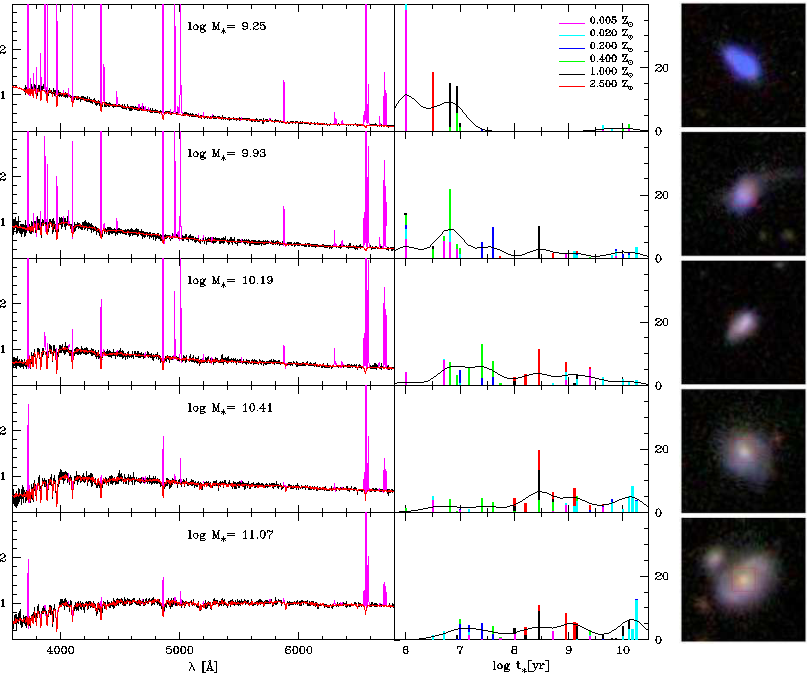
\includegraphics[width=1.0\textwidth]{figuras/starlight-fit.pdf}
	\caption[Exemplos de ajuste de espectro com o \starlight.]
	{Exemplos de ajuste de espectros de galáxias com o \starlight
	\citep{Asari2007}. À esquerda, espectros observados (preto), espectros
	modelados (vermelho), com regiões mascaradas em magenta. No meio, a fração da
	luz associada à cada uma das 25 idades das SSPs usadas na síntese, com a curva
	representando a versão suavizada do histórico de formação estelar. À direita,
	imagens do \SDSS correspondentes às galáxias.}
	\label{fig:StarlightSpectrumSample}
\end{figure}

A aplicação imediata do resultado do \starlight é a remoção do contínuo estelar
para medir com maior precisão as linhas de emissão provenientes do gás, não
incluídas no modelo. É possível também estudar o vetor de população $\vec{x}$,
que representa a fração de luz proveniente de cada população estelar da base. De
forma alternativa, pode-se utilizar o vetor de fração de massa $\vec{\mu}$, que
se relaciona ao $\vec{x}$ através da relação massa--luminosidade de cada
elemento da base. Individualmente os componentes $x_j$ e $\mu_j$ dos vetores não
são confiáveis, pois há muita degenerescência nos elementos da base\fixme
(referência?). Porém, a informação contida nos vetores pode ser condensada,
gerando medidas físicas galáxia, como a taxa de formação estelar, a idade
estelar média e a metalicidade estelar média, os dois últimos ponderados por
luminosidade ($\vec{x}$) ou massa ($\vec{\mu}$), por exemplo. Estas medidas são
muito mais robustas, como foi demonstrado por \citet{CidFernandes2013b}.

Esta técnica foi aplicada a 926246 espectros de galáxias do \SDSS. As
propriedades físicas resultantes do \starlight, junto com as medidas de linhas
de emissão, foram disponibilizados como um banco de dados no {\em website}
\url{http://www.starlight.ufsc.br/}\fixme(referência?). Este banco de dados já
foi utilizado por dezenas de pesquisadores em todo o mundo, resultando em vários
artigos \citep[para citar alguns]{Bian2006, Liang2007, Peeples2009,
Lara-Lopez2009, Lara-Lopez2010} e teses \citep{Mateus2006, Gomes2009,
Asari2010}\fixme(atualizar).

\TODO Aplicação nos espectros provenientes do QBICK. Base GRANADA.
Máscara de linhas de emissão. Reconstruir os cubos: gancho pro próximo capítulo.

% End of this chapter



  % PyCASSO
  %%%%%%%%%%%%%%%%%%%%%%%%%%%%%%%%%%%%%%%%%%%%%%%%%%%%%%%%%%%%%%%%%
% Tese de Doutorado / Dept Fisica, CFM, UFSC                    %
% Andre@UFSC - 2014                                             %
%%%%%%%%%%%%%%%%%%%%%%%%%%%%%%%%%%%%%%%%%%%%%%%%%%%%%%%%%%%%%%%%%

%:::::::::::::::::::::::::::::::::::::::::::::::::::::::::::::::%
%                                                               %
%                          Capítulo 3                           %
%                                                               %
%:::::::::::::::::::::::::::::::::::::::::::::::::::::::::::::::%

%***************************************************************%
%                                                               %
%                            PyCASSO                            %
%                                                               %
%***************************************************************%

\chapter{PyCASSO}
\label{sec:pycasso}

A fim de agilizar o desenvolvimento de ferramentas de manipulação de cubos de
dados do CALIFA. Este ``kit de ferramentas'' foi chamado de PyCASSO (Python
CALIFA \starlight Synthesis Organizer). PyCASSO foi desenvolvido em Pyton e é, a
grosso modo, composto de três partes.

Conversor de tabelas. Com ele se pode converter a saída do \starlight (arquivos
ASCII para cada pixel de cada galáxia) para cubos de dados nos formatos FITS e
HDF5, de forma a otimizar o acesso aos dados. Uma galáxia leva tipicamente 2
minutos para ser carregada em memória usando arquivos texto. Este tempo se reduz
para menos de um segundo usando arquivo FITS. Há outra otimização para acessar
dados de várias galáxias simultaneamente, utilizando o formato HDF5. Neste caso
a carga dos dados em disco para a memória é ``preguiçosa'', quer dizer, é feita
somente quando os dados são efetivamente acessados.

Camada de entrada e saída. Os arquivos FITS e HDF5 foram montados de forma a
serem facilmente acessados em qualquer ambiente. Ainda assim, há uma camada de
abstração de armazenamento, onde as várias matrizes e cubos são acessadas com
nomes próprios (por exemplo, \texttt{popx},que designa a fração de luz
distribuída pelas populações estelares), de forma a ser possível programar
ferramentas de análise sem precisar se preocupar com as características de cada
formato de armazenamento.

Camada de análise. Como foi mencionado na Seção \ref{sec:Intro:Sintese}, o
resultado da síntese consiste em cubos indexados por zona. Os dados ficam
armazenados no disco desta forma. Porém, na grande maioria das vezes se está
interessado na informação espacialmente resolvida. Esta camada implementa uma rotina de
conversão da notação de zonas para $(x, y)$. Boa parte das propriedades da
síntese, como luminosidade, massa, atenuação por poeira, e idade estelar, já
estão implementadas. Estes cubos espacialmente resolvidos são calculados
dinamicamente, quer dizer, não ocupam memória do sistema até que sejam
acessados. Existem outras rotinas para calcular geometria, perfis radiais e
azimutais, e raio de escala. Outras rotinas podem ser adicionadas
facilmente\footnote{Há um estudo de PCA (análise de componentes principais)
sendo desenvolvido por outro estudante na UFSC, por exemplo.}.

Este software está sendo utilizado pelo grupo de populações estelares da
colaboração do CALIFA, do qual o autor faz parte. No total são aproximadamente
10 pessoas utilizando este software. Foram publicados 4 artigos que utilizam
extensivamente PyCASSO, apresentados na Seção \ref{sec:pycasso:art}, e 2 que
utilizaram algum dado resultante de forma indireta \citep{Husemann2013,
IglesiasParamo2013}.


%***************************************************************%
%                                                               %
%                     PyCASSO - Ferramenta                      %
%                                                               %
%***************************************************************%

\section{A ferramenta de manipulação de cubos de dados PyCASSO}
\label{sec:pycasso:Pycasso}

PyCASSO é uma biblioteca desenvolvida em Python. Porém uma biblioteca não é nada
sem uma boa documentação. Aqui se apresenta de forma breve das capacidades do
PyCASSO. A documentação completa se encontra no Apêndice \ref{apendice:manual}.

O trabalho com a variedade e quantidade de dados gerados pela síntese espectral
de IFS tem em geral um caráter fortemente exploratório. Frequentemente não se
sabe exatamente o que se está buscando, e o trabalho do programador/cientista
consiste em desenhar gráficos, realizar cálculos, determinar operações ou
filtros nos dados com base nestes gráficos e cálculos, desenhar novamente, e
assim sucessivamente. Assim se escolheu a linguagem Python, que possui
ferramentas adequadas à programação exploratória\footnote{Além de estar se
tornando uma espécie de {\em lingua franca} na Astrofísica computacional.}, como
o \texttt{IPython}\footnote{\url{http://ipython.org/}} e o
\texttt{matplotlib}\footnote{\url{http://matplotlib.org/}}. Foi feito um esforço
para que o acesso aos dados de cada galáxia fosse feito de forma simples e
direta, um exemplo de código pode ser visto na Figura \ref{fig:dataAccess}.

\begin{figure}
\begin{python}
# Carregar arquivo FITS com os dados.
from pycasso import fitsQ3DataCube
K = fitsQ3DataCube('K0001_synthesis_suffix.fits')

# Acessar a idade media ponderada pela luminosidade.
at = K.at_flux__z

# Calcular a idade media da galaxia.
at_total = (at * K.Lobn__z).sum() / K.Lobn__z.sum()
print 'Idade media da galaxia: %.2f' % at_total
\end{python}
	\caption[Exemplo de programa utilizando PyCASSO]
	{Exemplo de acesso aos dados. Todas as propriedades estão disponíveis
	diretamente pelo nome, inclusive utilizando a função auto-completar da maioria
	dos ambientes de desenvolvimento Python.}
	\label{fig:dataAccess}
\end{figure}

Para algumas operações, como o cálculo da idade estelar média feito na Figura
\ref{fig:dataAccess}, pode-se utilizar apenas o resultado para as zonas. Neste
caso, a idade estelar média é calculada usando a expressão $\langle \log t
\rangle^{gal}_L = \sum_z \langle \log t \rangle_{L,z} L_z / \sum_z L_z$, onde
$L_z$ é a luminosidade de cada zona e $\langle \log t \rangle_{L,z}$ é a idade
estelar média de cada zona. Entretanto, para tirar vantagem das informações
espaciais, é preciso converter as propriedades da notação de zona para imagem.
Por exemplo, o programa na Figura \ref{fig:programaMapaIdade} calcula a idade
estelar média espacialmente resolvida\footnote{O mapa de idade já está
previamente calculado, disponível através da propriedade
\texttt{at\_flux\_\_yx}. Esta conversão é feita explicitamente aqui para
ilustrar como a conversão pode ser feita para qualquer propriedade.}, e em
seguida desenha um gráfico da imagem gerada (Figura \ref{fig:mapaIdade}).

\begin{figure}
\begin{python}
# Carregar arquivo FITS com os dados.
from pycasso import fitsQ3DataCube
K = fitsQ3DataCube('K0001_synthesis_suffix.fits')

# Converter zonas para imagem.
at_image = K.zoneToYX(K.at_flux__z, extensive=False)

# Desenhar o mapa.
import matplotlib.pyplot as plt
plt.imshow(at_image)
plt.colorbar()
\end{python}
	\caption[Programa para desenhar o mapa da idade estelar média] {Programa
	para desenhar o mapa de idade estelar média ponderada pela luminosidade.}
	\label{fig:programaMapaIdade}
\end{figure}

\begin{figure}
	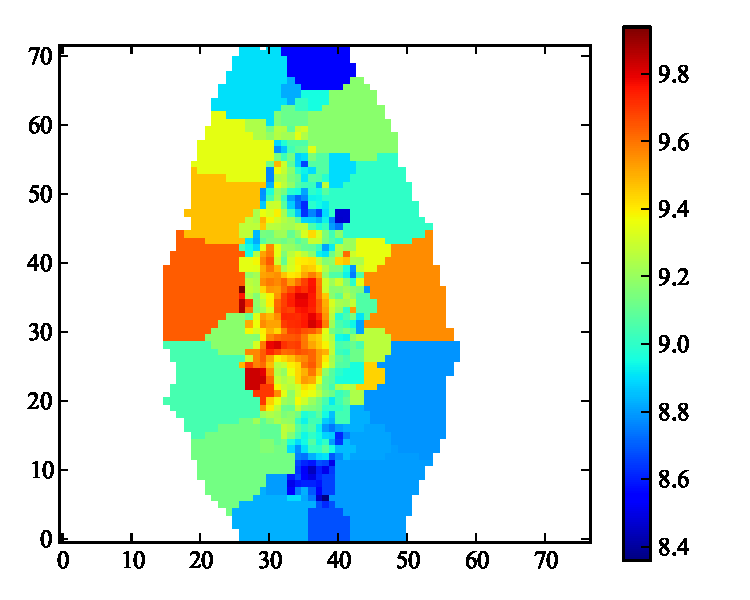
\includegraphics{figuras/mapa-idade}
	\caption[Mapa da idade estelar média da galáxia IC 5376] {Mapa de idade estelar
	média ponderada pela luminosidade da galáxia IC 5376, desenhado pelo programa
	da Figura \ref{fig:programaMapaIdade}.}
	\label{fig:mapaIdade}
\end{figure}

Enquanto um mapa é uma forma muito boa de visualizar informações em duas
dimensões, há vezes em que uma visualização resumida é mais adequada. Galáxias
em geral têm simetria aproximadamente axial, logo poder medir perfil radial das
propriedades das galáxias é fundamental para estudá-las. Com PyCASSO, o cálculo
do perfil radial é bastante simples, como pode ser visto no programa na Figura
\ref{fig:programaRadprofIdade}, que calcula o perfil radial da idade estelar
média. O resultado está na Figura \ref{fig:radprofIdade}.

\begin{figure}
\begin{python}
# Carregar arquivo FITS com os dados.
from pycasso import fitsQ3DataCube
K = fitsQ3DataCube('K0001_synthesis_suffix.fits')

# Converter zonas para imagem.
at_image = K.zoneToYX(K.at_flux__z, extensive=False)

# Calcular o perfil radial.
bins = np.arange(0, 26, 1)
bin_center = (bins[1:] + bins[:-1]) / 2.0
at_rad = K.radialProfile(at_image, bins, rad_scale=1.0)

# Desenhar o perfil radial.
import matplotlib.pyplot as plt
plt.plot(bin_center, at_rad)
\end{python}
	\caption[Programa para desenhar o perfil radial da idade estelar] {Programa
	para desenhar o perfil radial da idade estelar média ponderada pela
	luminosidade.}
	\label{fig:programaRadprofIdade}
\end{figure}

\begin{figure}
	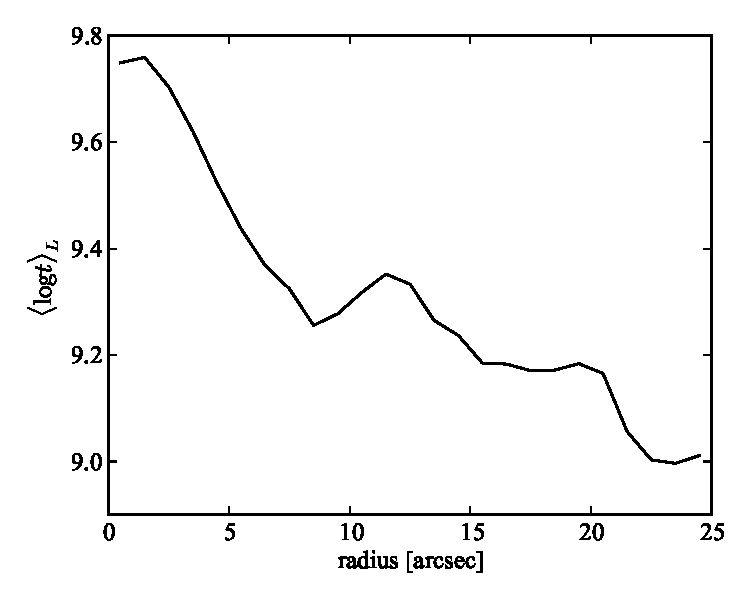
\includegraphics{figuras/radprof-idade}
	\caption[Perfil radial da idade estelar média da galáxia IC 5376] {Perfil
	radial da idade estelar média ponderada pela luminosidade da galáxia IC
	5376, desenhado pelo programa da Figura \ref{fig:programaRadprofIdade}.}
	\label{fig:radprofIdade}
\end{figure}

Esta é só uma pequena demonstração das ferramentas existentes no PyCASSO. Também
é possível trabalhar com espectros, calcular perfis azimutais, lidar com pixels
mascarados, entre outras coisas. Tudo isto está descrito em detalhes no manual
do programa (Apêndice \ref{apendice:manual}).


%***************************************************************%
%                                                               %
%                      PyCASSO - Artigos                        %
%                                                               %
%***************************************************************%

\section{Artigos publicados}
\label{sec:pycasso:art}

Nesta seção discute-se os artigos onde se utilizou PyCASSO, e o autor teve uma
colaboração importante. Além destes artigos, \citet{Husemann2013}, no artigo
apresentando o primeiro {\em data release}, utiliza as massas estelares
determinadas pelo \starlight e disponibilizadas pelo PyCASSO.


%***************************************************************%
%                                                               %
%       PyCASSO - Resolving galaxies in Space and Time I        %
%                                                               %
%***************************************************************%

\subsection{Artigo: {\em Resolving galaxies in time and space. I. Applying
STARLIGHT to CALIFA datacubes}}
\label{sec:pycasso:art:Resolving1}

Este artigo por \citet{CidFernandes2013a} descreve todo o processo de síntese
espectral dos cubos de dados do CALIFA, mencionados no Capítulo \ref{sec:intro},
e serve como uma demonstração da capacidade do PyCASSO. O artigo está
reproduzido na íntegra no Apêndice \ref{apendice:PaperResolving1}. O
preprocessamento dos cubos de espectros é feito através do programa QBICK,
desenvolvido por Rubén Garcia Benito especialmente para o CALIFA, mas é
genérico o bastante para ser usado em outros cubos de dados. Após explicar em
detalhes todos os passos envolvidos desde o preprocessamento, passando pela
descrição do \starlight até a importação dos dados pelo PyCASSO, o artigo
apresenta um caso de estudo com a galáxia NGC 2916.

\begin{figure}
	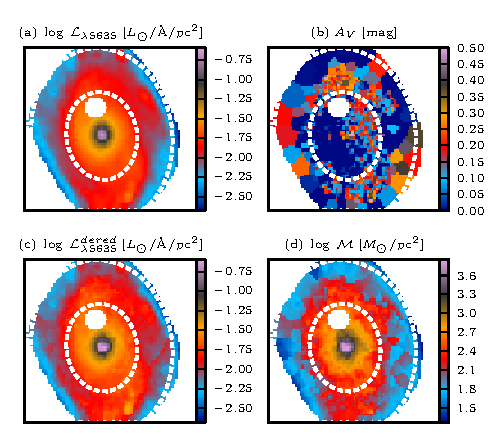
\includegraphics{figuras/L-M-AV-K0277}
	\caption[Propriedades físicas espacialmente resolvidas para a galáxia NGC
	2916] {Propriedades físicas espacialmente resolvidas para a galáxia NGC 2916. (a)
	Luminosidade em $5635\,\AA$ por unidade de área. (b) Atenuação por poeira na
	banda $V$. (c) Luminosidade em $5635\,\AA$ por unidade de área, corrigido de
	extinção. (d) Desidade superficial de massa estelar. Retirado de
	\cite[figura 4]{CidFernandes2013a}, Apêndice \ref{apendice:PaperResolving1}.}
	\label{fig:LMAVMap}
\end{figure}


\begin{figure}
	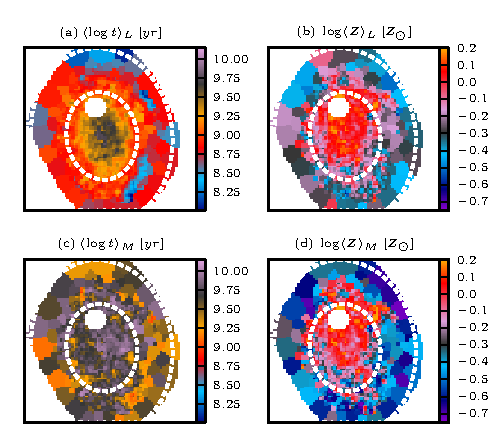
\includegraphics{figuras/at-aZ-K0277}
	\caption[Idade estelar e metalidade espacialmente resolvidas para a
	galáxia NGC 2916] {Idade e metalicidade estelar média, espacialmente
	resolvidas, para a galáxia NGC 2916. (a) Idade estelar média pesada pela
	luminosidade. (b) metalicidade estelar média pesada pela luminosidade.
	(c) Idade estelar média pesada pela massa. (d) metalicidade estelar
	média pesada pela massa. Retirado de
	\cite[figura 6]{CidFernandes2013a}, Apêndice \ref{apendice:PaperResolving1}.}
	\label{fig:ataZMap}
\end{figure}

% TODO: corrigir largura
\begin{figure}
	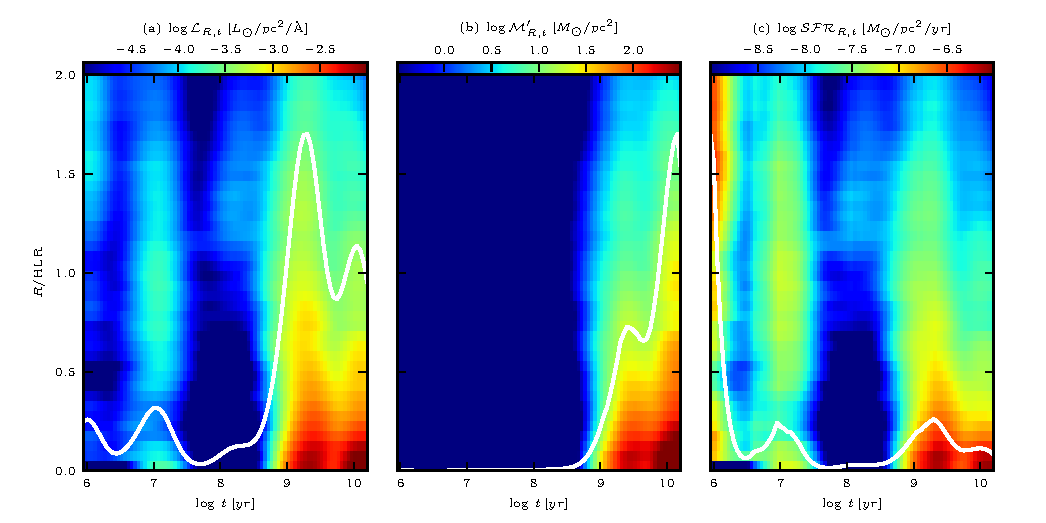
\includegraphics[width=1.0\columnwidth]{figuras/L-M-SFR-K0277}
	\caption[Diagramas $R \times t$ para luz, massa e SFR] {Diagramas $R \times t$
	para luz, massa e taxa de formação estelar (SFR). (a) Luminosidade em
	$5635\,\AA$ por unidade de área.  (b) Massa transformada em estrelas por
	unidade de área. (c) Taxa de formação estelar por unidade de área. A linha
	sólida representa o gráfico colapsado na direção vertical, apenas para ilustrar
	a variação temporal das quantidades mapeadas. Retirado de
	\cite[figura 12]{CidFernandes2013a}, Apêndice \ref{apendice:PaperResolving1}.}
	\label{fig:LMSFR2D}
\end{figure}

As Figuras \ref{fig:LMAVMap} e \ref{fig:ataZMap} mostram mapas de propriedades
físicas obtidas pela síntese espectral. Propriedades como a massa (Figura
\ref{fig:LMAVMap}d) e luminosidade (Figuras \ref{fig:LMAVMap}a e
\ref{fig:LMAVMap}c) são quantidades extensivas, e são proporcionais à escala. Já
a atenuação por poeira (Figura \ref{fig:LMAVMap}b), idade e metalicidade estelar
são quantidades intensivas, independentes de escala. Na prática isto significa
que as quantidades extensivas podem ser divididas entre os pixels que compõem
uma zona, enquanto as intensivas são uma propriedade comum à todos os pixels
desta zona. Esta diferença pode ser notada nas zonas mais externas dos mapas,
onde aparecem platôs na quantidades intensivas. As quantidades extensivas passam
por um processo apelidado de ``dezonificação''\fixme, descrito na Seção
\ref{sec:pycasso:Pycasso}.

Um dos desafios de se trabalhar com cubos multidimensionais é como visualizar
esta informação. Uma alternativa é comprimir determinadas dimensões. Para
ilustrar esta capacidade do PyCASSO, a Figura \ref{fig:LMSFR2D} mostra diagramas
de luz, massa e taxa de formação estelar (SFR) em função do tempo, onde as
dimensões $x$ e $y$ foram transformadas em distância radial. Diagramas como
este, junto com perfis 1-D radiais e temporais ajudam a visualizar e interpretar
o resultado da síntese espectral, oferecendo novas ferramentas para estudar a
estrutura e evolução de galáxias.


%***************************************************************%
%                                                               %
%       PyCASSO - Resolving galaxies in Space and Time II       %
%                                                               %
%***************************************************************%

\subsection{Artigo: {\em Resolving galaxies in time and space: II: Uncertainties
in the spectral synthesis of datacubes}}
\label{sec:pycasso:art:Resolving2}

Uma crítica bastante comum aos métodos de ajuste é que eles não provêm a
incerteza associada aos valores ajustados. A forma mais simples de determinar
esta incerteza é refazer o ajuste várias vezes, perturbando as medidas
reproduzindo de forma realista os erros. Este artigo por
\citet{CidFernandes2013b} investiga a incerteza nos ajustes feitos no artigo
discutido na seção anterior. O artigo está reproduzido na íntegra no Apêndice
\ref{apendice:PaperResolving2}.

Quando se injeta erros aleatórios, obtém-se incertezas de $\sim
0.08\,\mathrm{dex}$ em idades e metalicidades pesadas pela luminosidade, e de
$\sim 0.15\,\mathrm{dex}$ quando pesadas pela massa. A massa estelar teve uma
incerteza de $\sim 0.08\,\mathrm{dex}$, e $A_V$ de $\sim 0.06\,\mathrm{mag}$.
Injetando erros sistemáticos em cor\footnote{Adicionando componentes lineares em
comprimento de onda, a fim de emular uma má calibração de fluxo.} os erros são
similares, exceto para $A_V$, que recebe um desvio sistemático de
$+0.05\,\mathrm{mag}$ e um erro de $\sim 0.16\,\mathrm{mag}$.

\begin{figure}
	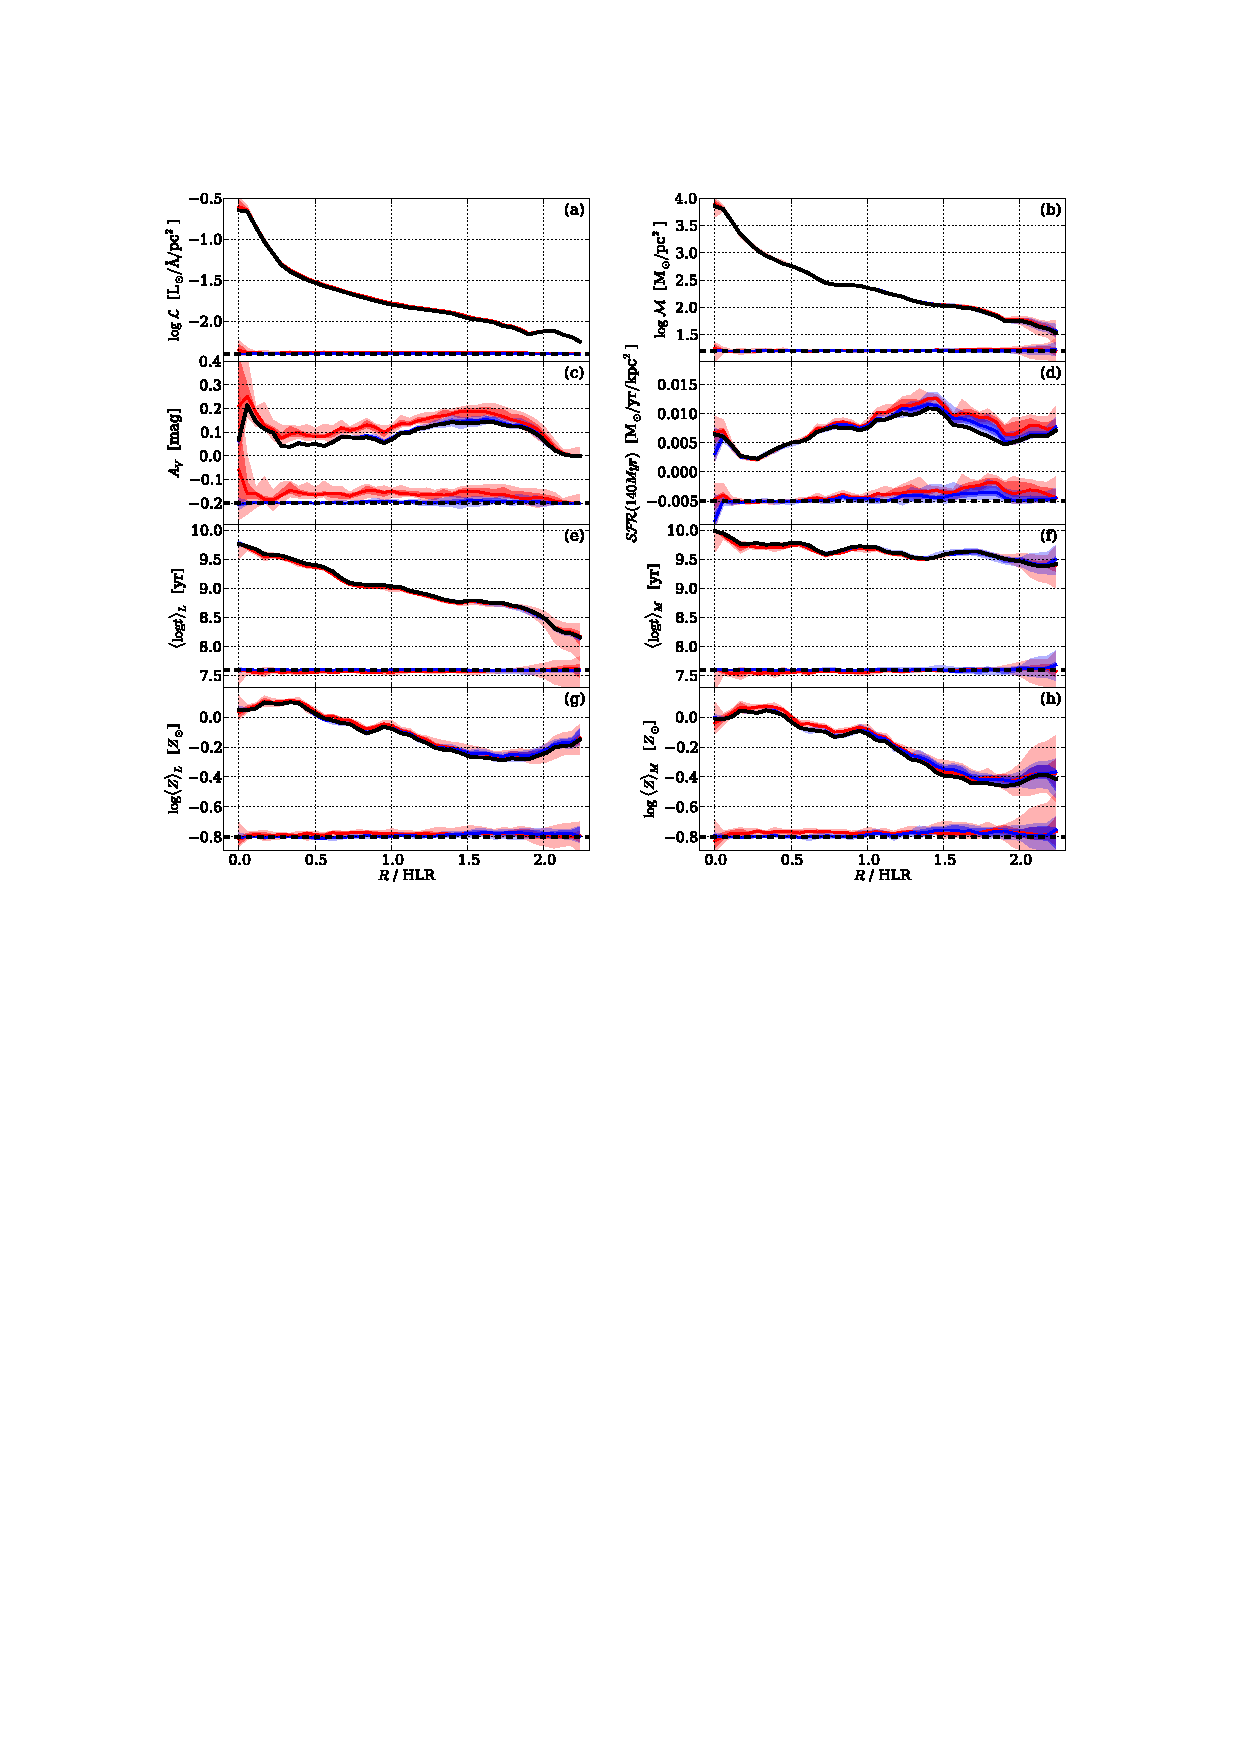
\includegraphics[width=1.0\columnwidth]{figuras/resolving2}
	\caption[Incerteza nos perfis radiais] {Incerteza nos perfis radiais de
	algumas propriedades. (a) Luminosidade superficial a $5635\,\AA$, corrigida de
	extinção. (b) Densidade superficial de massa. (c) Atenuação na banda $V$. (d)
	Taxa de formação estelar (últimos $140\, \mathrm{Myr}$) por unidade de área.
	(e) Idade estelar média ponderada pela luminosidade. (f) Idade estelar média
	ponderada pela massa. (g) Metalicidade estelar média ponderada pela
	luminosidade. (h) Metalicidade estelar média ponderada pela massa. As
	linhas em preto marcam a solução original. Em faixas azuis e vermelhas, as
	distribuições das realizações com ruído aleatório, e sistemático em cor,
	respectivamente. A diferença entre as simulações e o original está desenhada
	abaixo de cada painel, com o zero marcado pela linha tracejada. Retirado de
	\cite[figura 4]{CidFernandes2013b}, Apêndice \ref{apendice:PaperResolving2}.}
	\label{fig:incertRad}
\end{figure}

Embora haja uma incerteza considerável analisando-se as propriedades da galáxia
pixel a pixel, os perfis radiais em geral são bastante robustos. Propriedades
diretas como a luminosidade, massa, idade e metalicidade estelar, quando vistas
em perfil radial (Figura \ref{fig:incertRad}) mantém o mesmo formato com pouca
dispersão, exceto nas regiões mais afastadas do núcleo, onde há poucas zonas. Na
verdade, qualquer forma de média espacial que envolva pixels (ou zonas)
suficientes deverá levar a uma diminuição na incerteza.

% FIXME: corrigir largura da figura
\begin{figure}
	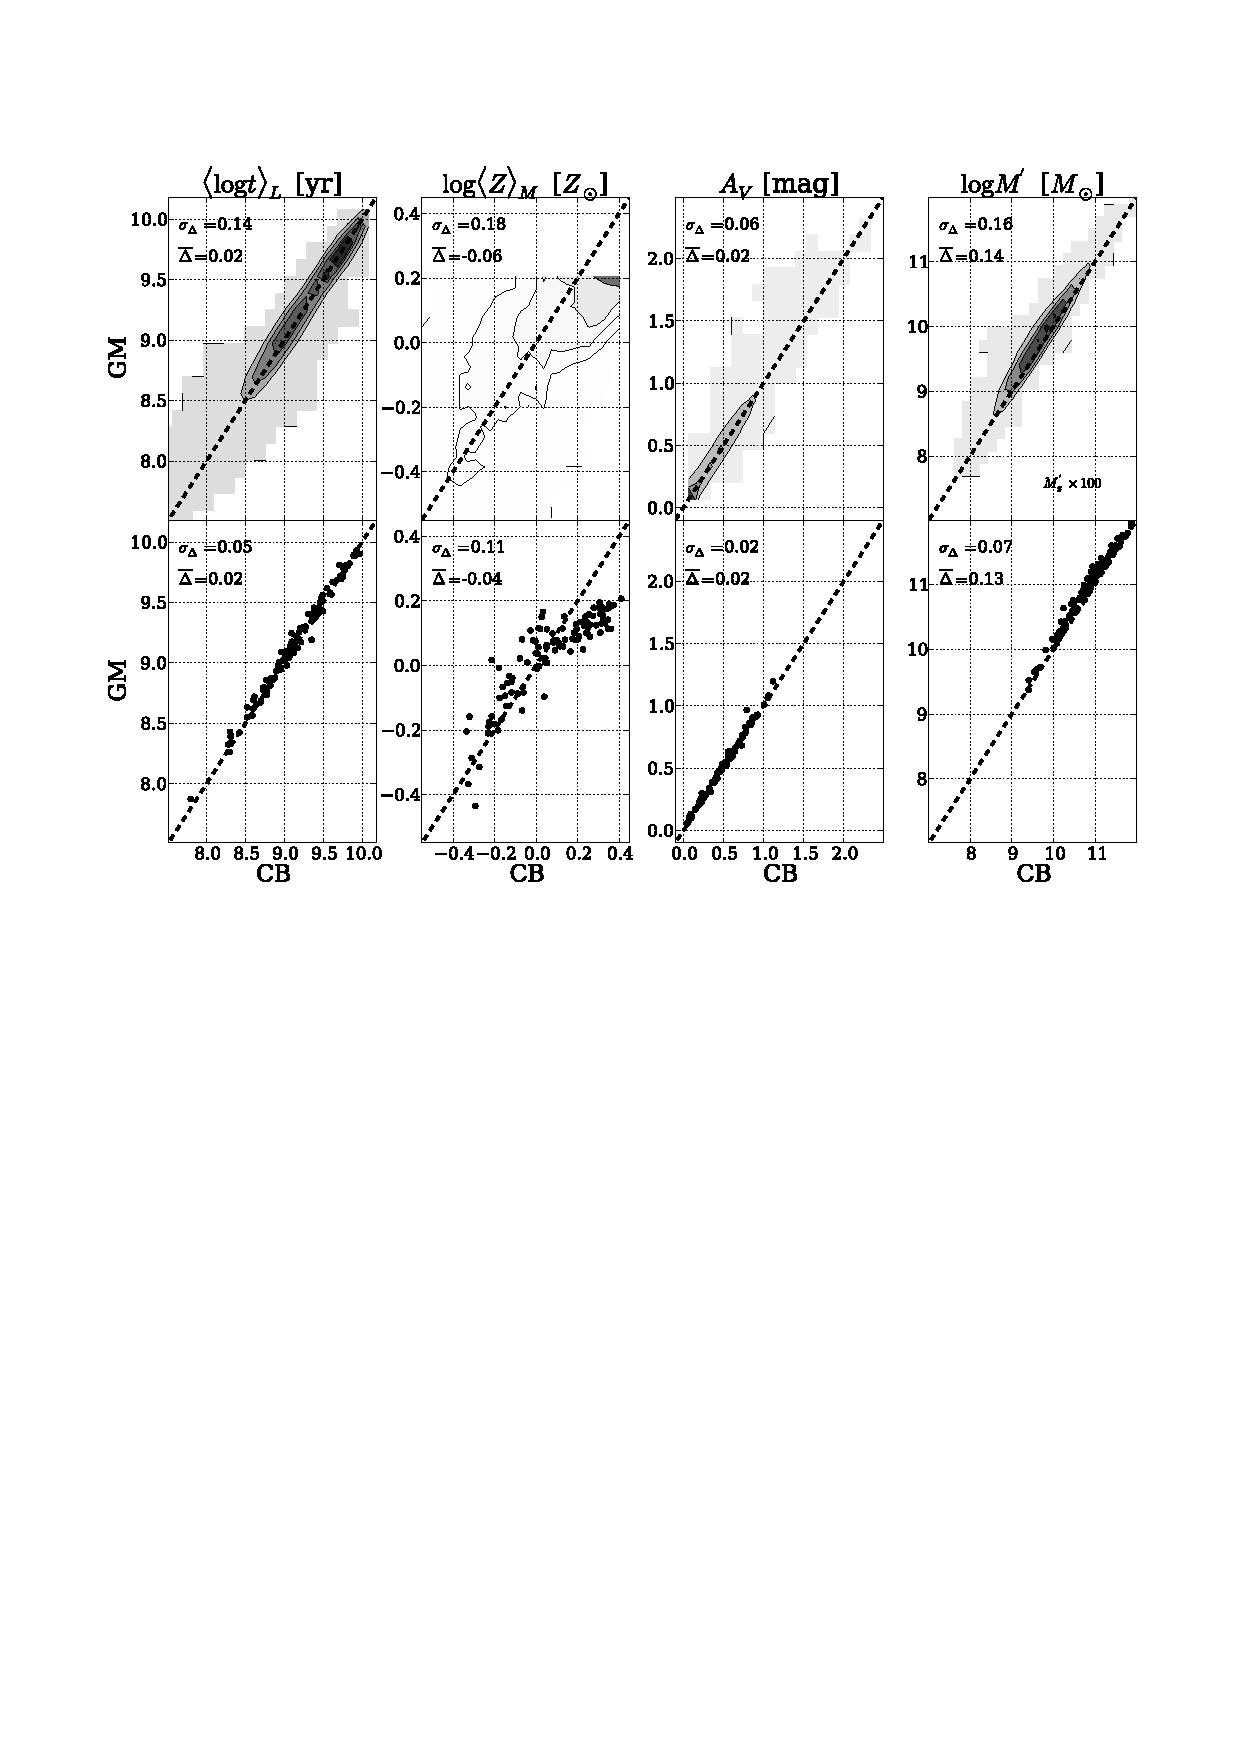
\includegraphics[width=1.0\columnwidth]{figuras/resolving2-base}
	\caption[Comparação dos ajustes com bases de SSP diferentes]
	{Comparação de propriedades obtidas com o ajuste utilizando as bases
	GM (eixo vertical) CB (eixo horizontal). Os painéis superiores mostram um
	histograma 2-D com contornos para propriedades de cada pixel de 107 galáxias do
	CALIFA. Da esquerda para a direita: idade estelar ponderada pela luminosidade,
	metalicidade estelar ponderada pela massa, atenuação na banda $V$, massa
	estelar inicial. Os painéis inferiores mostram a distribuição das mesmas
	propriedades, porém calculadas para o espectro integradas das galáxias.
	Retirado de \cite[figura 9]{CidFernandes2013b}, Apêndice
	\ref{apendice:PaperResolving2}.}
	\label{fig:incertRad-base}
\end{figure}

O artigo também explora os efeitos da escolha da base de SSPs nos resultados do
ajuste. Em geral, bases diferentes levam a resultados consistentes.
Pode-se ver na Figura \ref{fig:incertRad-base} que a idade estelar
média ponderada pela luminosidade, a atenuação e a massa estelar inicial
têm uma concordância muito boa entre as bases. As metalicidades médias mostram
uma correlação, mas com uma dispersão muito grande, certamente devido a
diferenças nas trajetórias evolucionárias dos modelos, poucos valores
de metalicidade na base, e diferenças na metalicidade máxima da base. A
incerteza nestas propriedades mencionadas acima é cerca de $2$ vezes maior do
que as calculadas adicionando ruído aleatório. Claramente a escolha de uma base
adequada é de grande importância para a análise.


%***************************************************************%
%                                                               %
%                 PyCASSO - Inside-out growth                   %
%                                                               %
%***************************************************************%

\subsection{Artigo: {\em The Evolution of Galaxies Resolved in Space and Time: A
View of Inside-out Growth from the CALIFA Survey}}
\label{sec:pycasso:art:InsideOut}

Em \citet{Perez2013} se estuda o crescimento de dentro para fora de $105$
galáxias do CALIFA. O estudo se baseia na síntese espectral com o \starlight, e
segue exatamente a mesma prescrição de \citet{CidFernandes2013a}, descrita na
Seção \ref{sec:pycasso:art:Resolving1}. O artigo está reproduzido na íntegra no
Apêndice \ref{apendice:InsideOut}.

Galáxias vêm em todos os tamanhos. Para determinar o crescimento, as distâncias
são normalizadas em utilizando o raio onde a luminosidade cumulativa (em
$5635\,\AA$) alcança $50\%$ da luminosidade total da galáxia, denominado
$R_{50}$. As galáxias da amostra são separadas em {\em bins} com $15$ galáxias
cada, segundo a sua massa. O crescimento em massa em função do tempo é calculado
para cada pixel de cada galáxia e somado em cada {\em bin} de massa.

\begin{figure}
	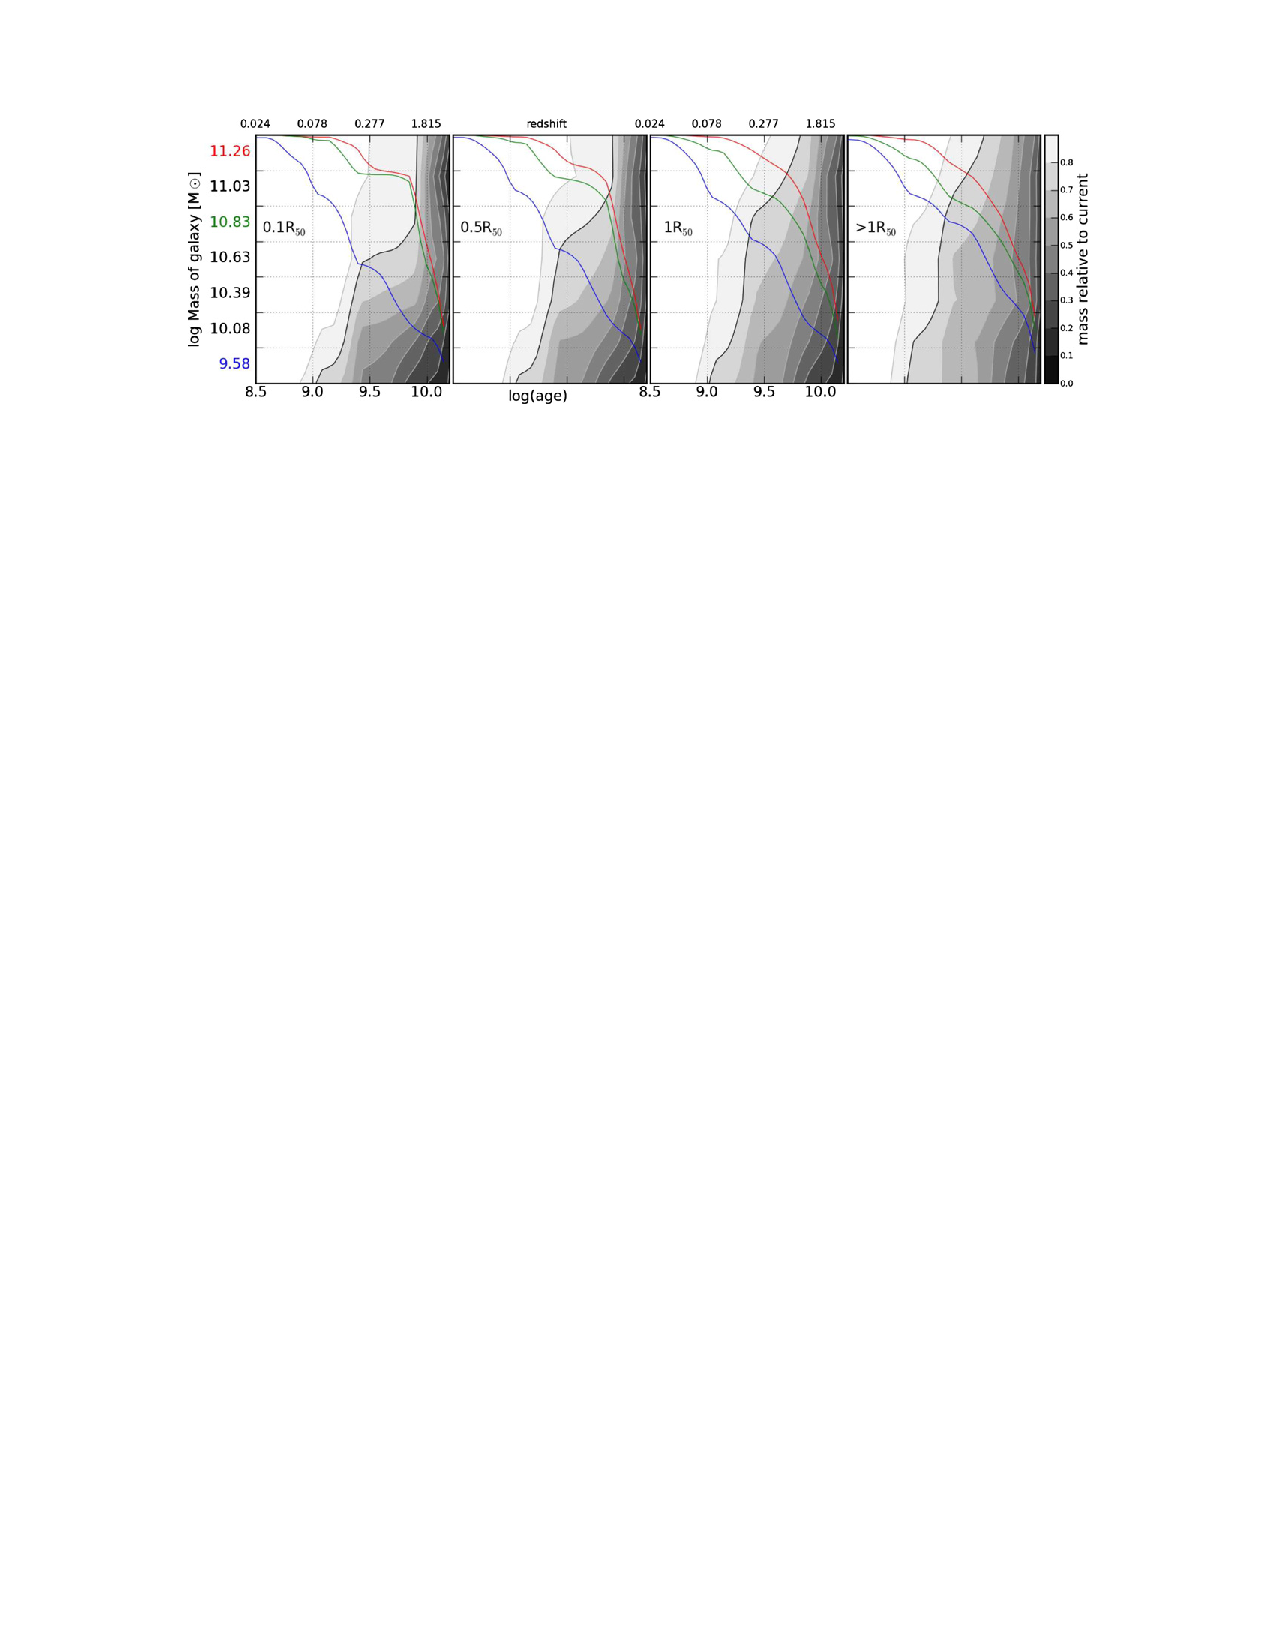
\includegraphics{figuras/inside-out}
	\caption[Crescimento da massa estelar de galáxias de dentro para fora]
	{Crescimento de massa estelar de dentro para fora. As $105$ galáxias foram
	separadas em grupos de 15, em massa, formando os {\em bins} do eixo vertical.
	Os painéis mostram o crescimento da massa em escala de cinza, normalizado, em
	função do tempo e da massa das galáxias. O contorno em preto marca $80\%$. Da
	direita para a esquerda se vê as regiões em raio $r < 0,1\,R_{50}$, $0,1 < r
	\leq 0,5\,R_{50}$, $0,5 < r \leq 1\,R_{50}$ e $r > 1\,R_{50}$. Para
	facilitar a visualização da forma da variação temporal, as linhas azuis, verdes
	e vermelhas em cada painel mostram um corte horizontal nos {\em bins} inferior,
	intermediário e superior, com escala de $0$ a $1$. Retirado de \cite[figura
	9]{Perez2013}, Apêndice \ref{apendice:InsideOut}.}
	\label{fig:insideOut}
\end{figure}

A Figura \ref{fig:insideOut} ilustra o crescimento de massa em anéis crescentes
em raio ($0,1\,R_{50}$, $0,5\,R_{50}$, $1\,R_{50}$ e $>1\,R_{50}$.). Em cada
painel, o tempo passa da direita para a esquerda, e a massa estelar,
normalizada, cresce desde zero (direita, em preto) até $1$ (esquerda, em
branco). Se vê claramente que galáxias menos massivas, na parte inferior dos
{\em bins}, têm um crescimento gradual mais ou menos constante em todos os
raios. As galáxias mais massivas, a parte superior dos {\em bins}, apresentam um
crescimento muito rápido nas regiões centrais, enquanto as regiões externas
crescem mais gradualmente. As linhas azul, verde e vermelha, em cada painel,
representam cortes horizontais no {\em bin} de mais baixa massa, no
intermediário e no de mais alta massa, respectivamente, para facilitar a
visualização. A mudança de regime ocorre em $\log M\star = 10,83$, ou seja, uma
massa de $\sim 7\times10^{10}\,M_\odot$. O autor cita vários estudos que indicam
esta faixa como uma ``massa especial'', onde a taxa de formação estelar alcança
valores altos muito rapidamente. De qualquer forma, esta é uma evidência
observacional de algo que já se suspeita há muito tempo:
que as galáxias massivas se formaram de dentro para fora.


%***************************************************************%
%                                                               %
%                 PyCASSO - Radial structures                   %
%                                                               %
%***************************************************************%

\subsection{Artigo: {\em The star formation history of CALIFA galaxies: Radial
structures}}
\label{sec:pycasso:art:RadStruct}

O artigo por \citet{GonzalezDelgado2013} faz um estudo detalhado da estrutura
radial de diversas propriedades de $107$ galáxias do CALIFA. O artigo está
reproduzido na íntegra no Apêndice \ref{apendice:RadStruct}.
Um dos resultados mais importantes é que a densidade superficial de massa
estelar e idade estelar média ponderada por luminosidade, medidas a $1\,R_{50}$,
são representativos das médias da galáxia como um todo. A Figura
\ref{fig:radStruct1} mostra a correlação entre os valores em três raios
distintos e o global para a idade estelar média ponderada pela luminosidade
(esquerda) e a densidade superficial de massa estelar (centro). Valores a
$1\,R_{50}$, marcado como HLR ({\em Half Light Radius}) nas figuras, coincidem
em geral com a média global da galáxia.
Ainda na mesma figura pode-se ver a correlação entre a densidade superficial de
massa estelar média da galáxia e a massa estelar total da galáxia. Este
resultado está de acordo com \citet{Kauffmann2003}, usando a amostra do SDSS.

\begin{figure}
	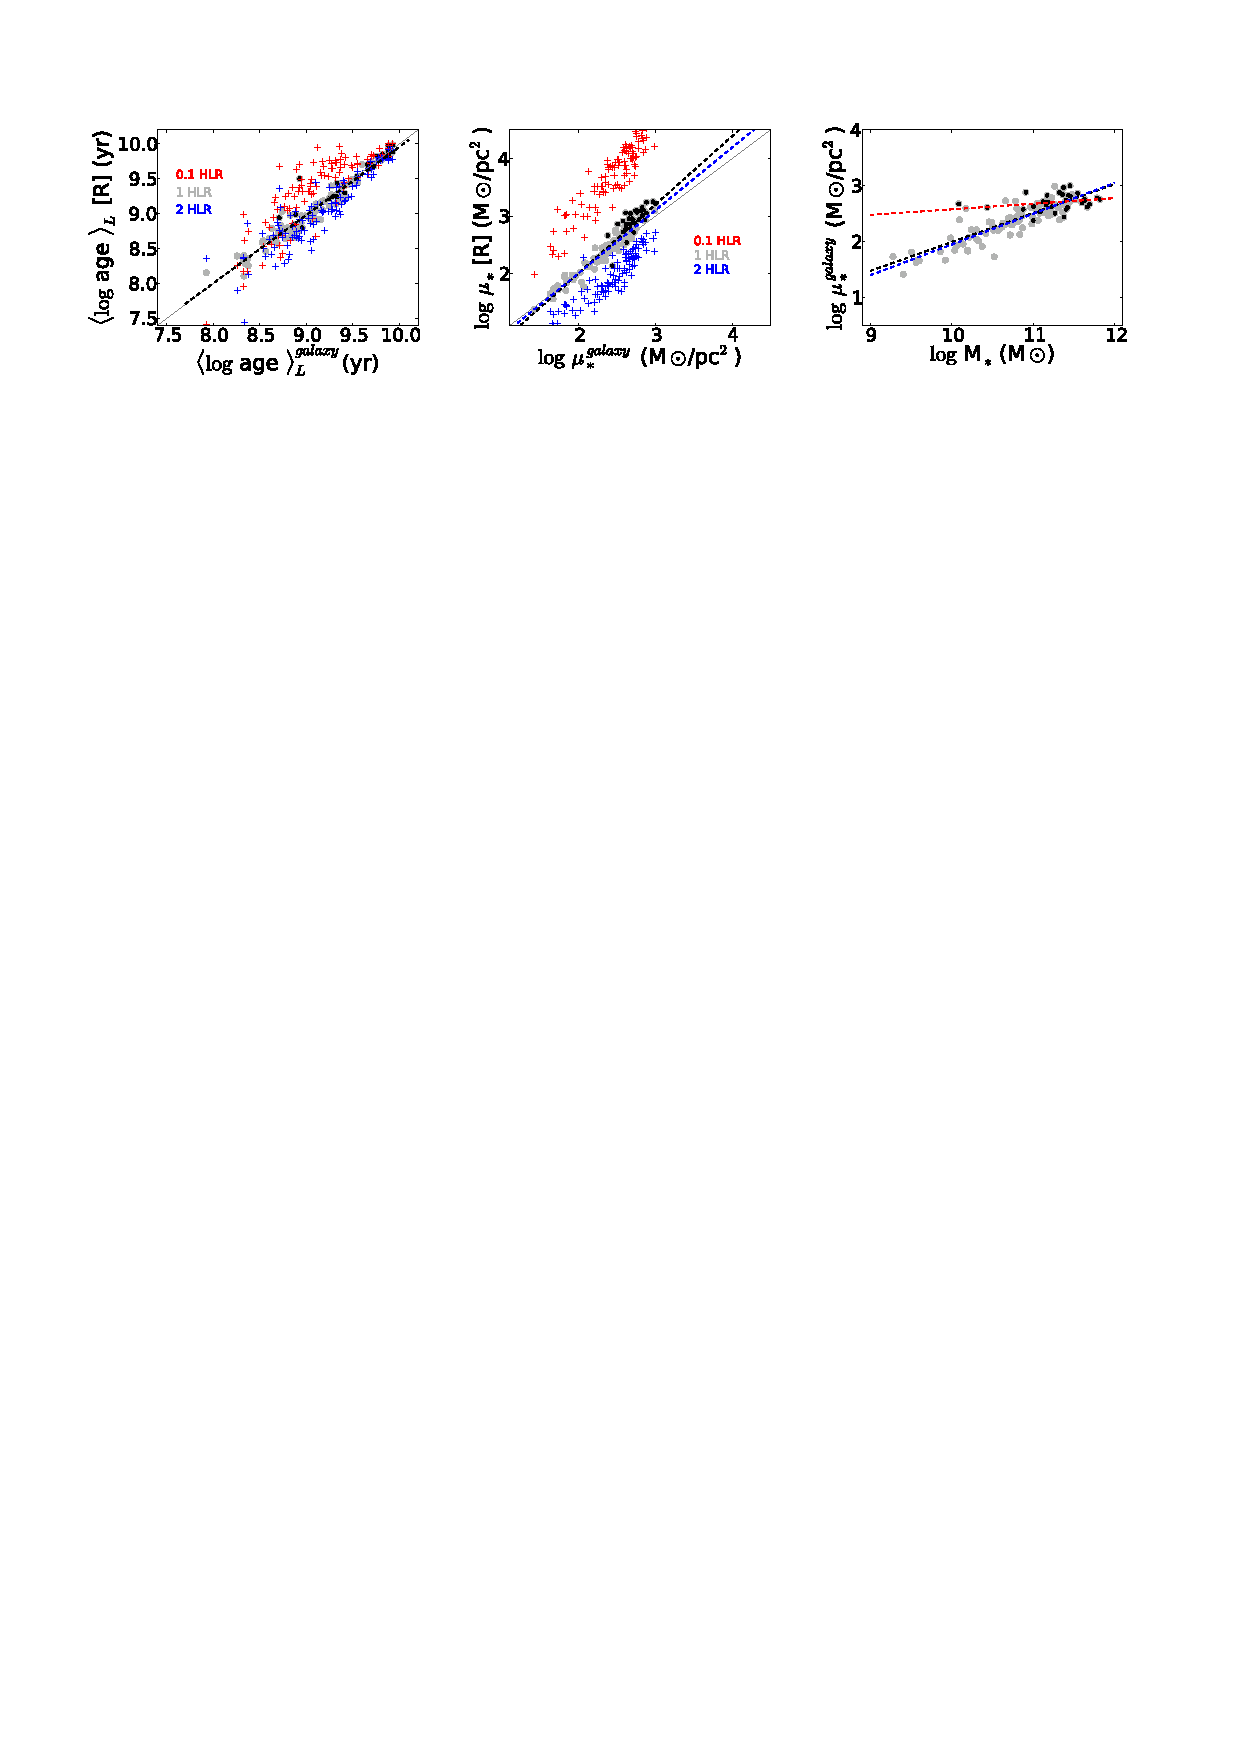
\includegraphics[width=1.0\columnwidth]{figuras/radstruct-01}
	\caption[Correlação entre idade, desidade superficial e massa estelar total]
	{(esquerda) Correlação entre a idade estelar média ponderada pela luminosidade
	em $1\,R_{50}$ (círculos cinza), $0,1\,R_{50}$ (cruzes azuis), $2\,R_{50}$
	(cruzes vermelhas) e a média da galáxia. Pontos em preto marcam galáxias
	esferoidais, com $C \geq 2,8$. (centro) O mesmo gráfico para a densidade
	superficial de massa estelar. (direita) Correlação entre a densidade
	superficial de massa média da galáxia e a massa estelar total da galáxia. As
	linhas tracejadas mostram o ajuste linear total (preto), apenas discos (azul),
	e apenas para esferoidais (vermelho).  Retirado de \cite[figura
	6]{GonzalezDelgado2013}, Apêndice \ref{apendice:RadStruct}.}
	\label{fig:radStruct1}
\end{figure}

O raio contendo metade da massa estelar (HMR, {\em Half Mass Radius}) é em média
20\% menor que $R_{50}$ (HLR). A razão entre HMR e HLR tem correlação com a
massa total da galáxia e o tipo morfológico. Na Figura \ref{fig:radStruct2}
pode-se ver que a relação HMR/HLR diminui com a massa estelar para galáxias com
massa menor que $10^{11}\,M_\odot$, enquanto permanece constante para galáxias
mais massivas. Um comportamento similar ocorre com o tipo morfológico:
em galáxias com disco a relação HMR/HLR diminui com a massa, e em galáxias
esferoidais a relação é aproximadamente constante.

\begin{figure}
	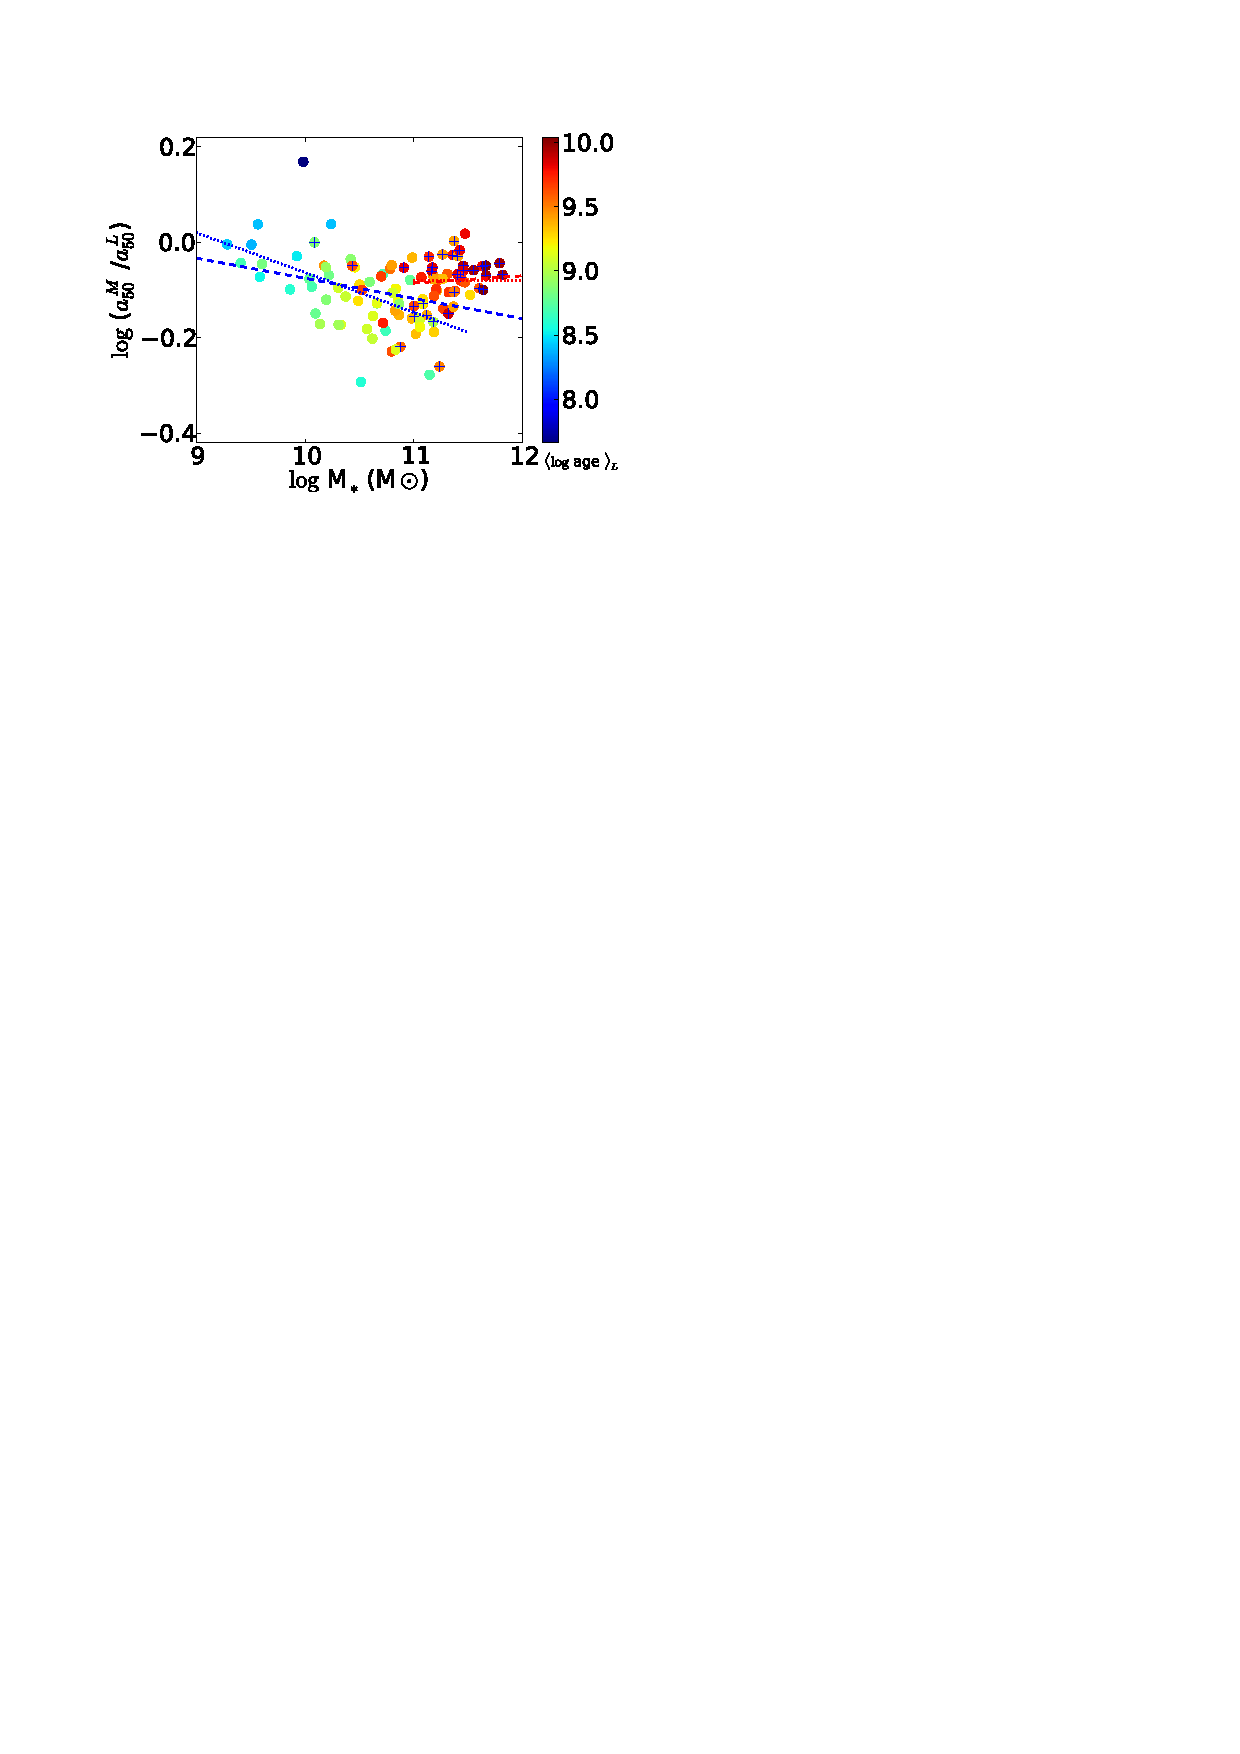
\includegraphics{figuras/radstruct-02}
	\caption[Relação entre $a^M_{50}/a^L_{50}$ e a massa estelar total]
	{Relação entre $a^M_{50}/a^L_{50}$ e a massa estelar total. A cor dos
	pontos reflete a idade estelar média ponderada pela luminosidade, em $0,5\,a^L_{50}$.
	Galáxias com índice de concentração $C \geq 2,8$ estão marcadas com uma cruz. A
	linha azul mostra o ajuste linear para galáxias com massa estelar Retirado de
	\cite[figura 10]{GonzalezDelgado2013}, Apêndice
	\ref{apendice:RadStruct}.}
	\label{fig:radStruct2}
\end{figure}

Para galáxias esferoidais, o gradiente de idade depende mais da massa estelar
total da galáxia do que da densidade superficial de massa estelar, que, conforme
o painel inferior esquerdo da Figura \ref{fig:radStruct3}, é aproximadamente
constante. A massa total da galáxia é a propriedade mais fundamental para
galáxias esferoidais, enquanto a densidade superficial de massa é mais
importante para as galáxias com disco.


\begin{figure}
	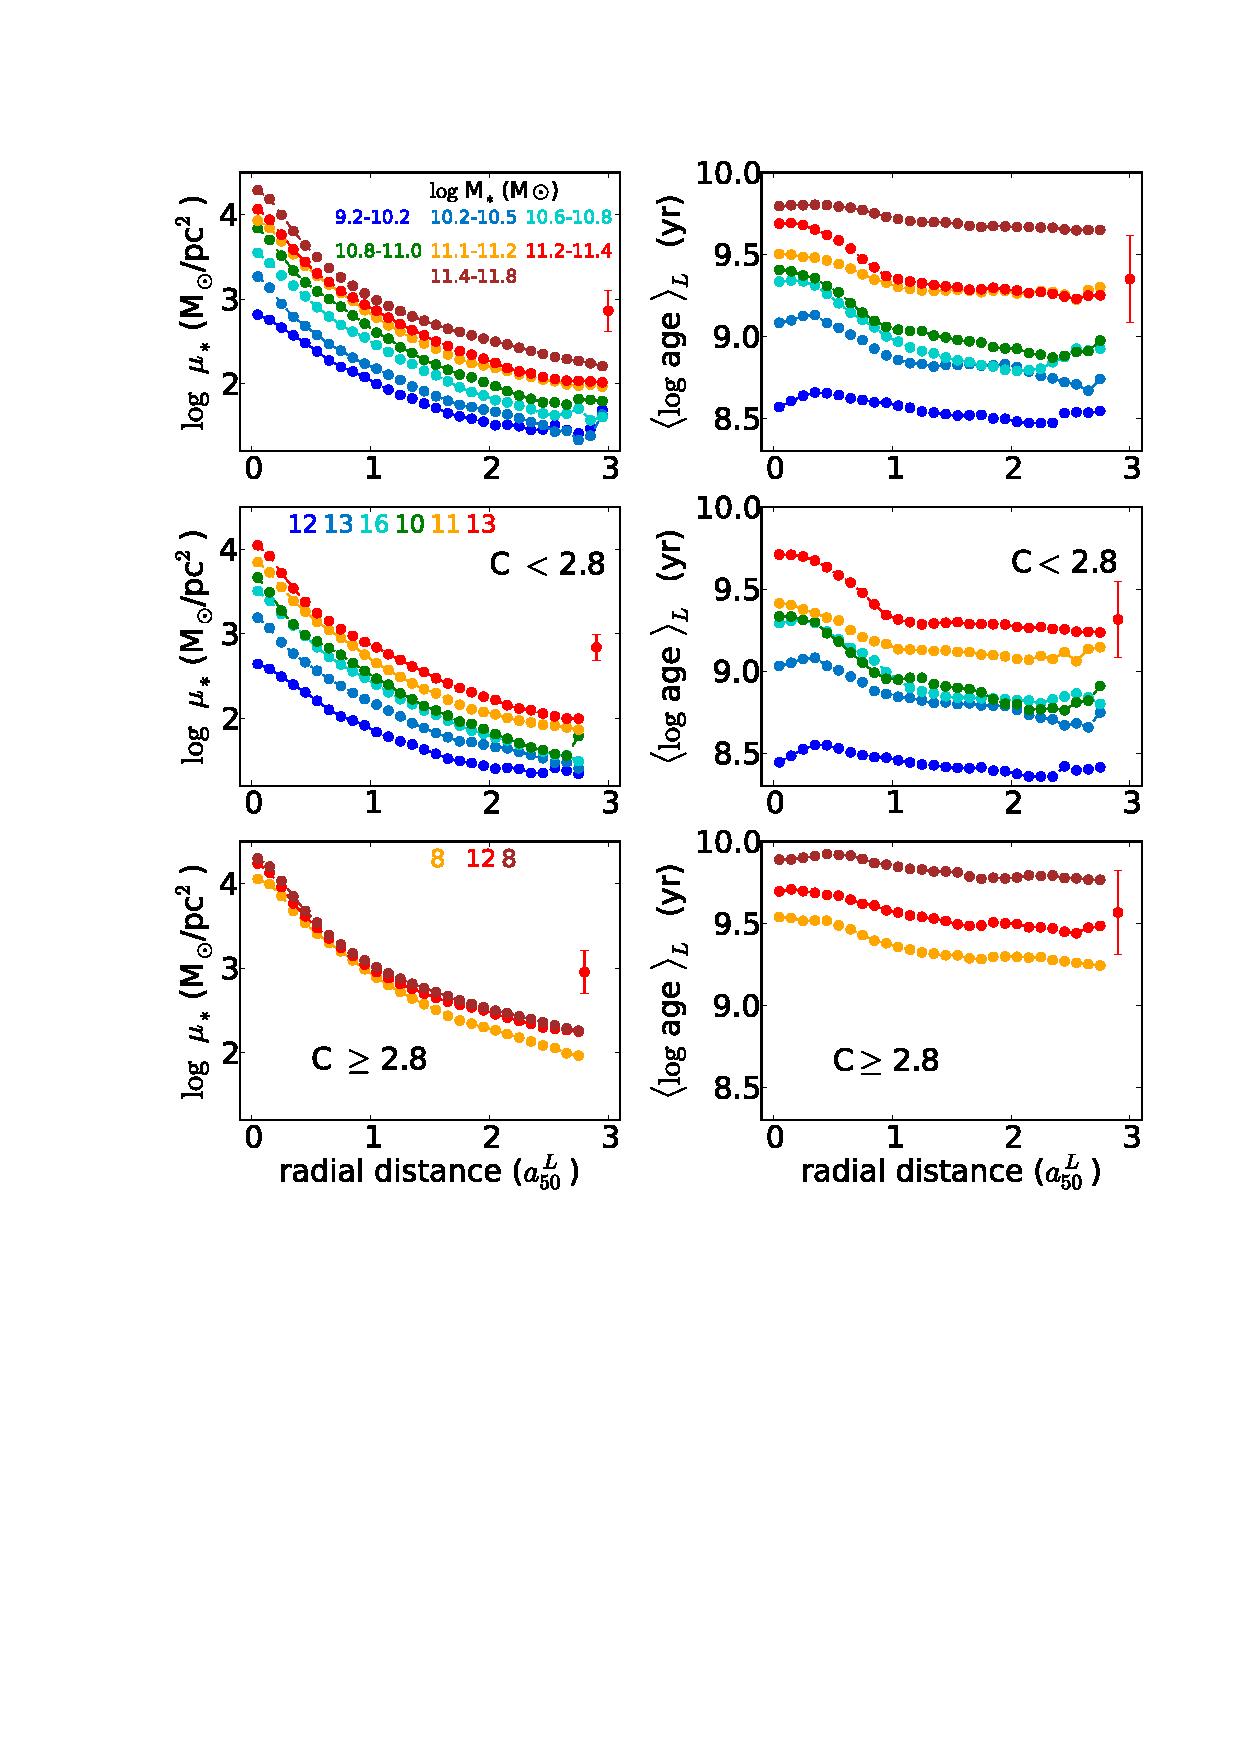
\includegraphics[width=0.8\columnwidth]{figuras/radstruct-03}
	\caption[Perfis radiais para vários {\em bins} de massa estelar.]
	{Perfis radiais da densidade superficial de massa estelar (esquerda) e idade
	estelar média ponderada pela luminosidade (direita), para {\em bins} de
	massa estelar contendo 15 galáxias cada. (cima) Todas as galáxias. Os {\em
	bins} em massa estão codificados em cores. (meio) Galáxias dominadas por
	disco. (baixo) Galáxias esferoidais ($C \geq 2,8$). Retirado de \cite[figura
	13]{GonzalezDelgado2013}, Apêndice \ref{apendice:RadStruct}.}
	\label{fig:radStruct3}
\end{figure}


% End of this chapter

  
  % Morfologia de galáxias
  %%%%%%%%%%%%%%%%%%%%%%%%%%%%%%%%%%%%%%%%%%%%%%%%%%%%%%%%%%%%%%%%%
% Qualificacao de Doutorado / Dept Fisica, CFM, UFSC            %
% Andre@UFSC - 2013                                             %
%%%%%%%%%%%%%%%%%%%%%%%%%%%%%%%%%%%%%%%%%%%%%%%%%%%%%%%%%%%%%%%%%


%:::::::::::::::::::::::::::::::::::::::::::::::::::::::::::::::%
%                                                               %
%                          Capítulo 4                           %
%                                                               %
%:::::::::::::::::::::::::::::::::::::::::::::::::::::::::::::::%

%***************************************************************%
%                                                               %
%                           Conclusao                           %
%                                                               %
%***************************************************************%

\chapter{Conclusões e perspectivas}
\label{sec:conclusao}

O survey CALIFA está produzindo cubos de dados de IFS de $600$ galáxias. Já
foram publicados $100$ destes cubos no primeiro {\em data release}, e mais de
$200$ foram observados, mas ainda estão em processo de controle de qualidade e
embargo da colaboração. Através do programa \starlight, foram obtidos diversos
parâmetros relacionado às populações estelares componentes de cada pixel,
formando cubos de dados adicionais ao observados. Neste trabalho, foi
desenvolvido um programa chamado PyCASSO para organizar e analisar estes cubos
de dados. Este programa é utilizado por cerca de $10$ pessoas que estudam
populações estelares na colaboração do CALIFA. Bastante atenção foi dada à
documentação (\ref{sec:pycasso:Pycasso}), que pode ser vista no Apêndice
\ref{apendice:manual}. Foram publicados $4$ artigos que se baseiam fortemente no
uso de PyCASSO para análise e gráficos, resumidos na Seção \ref{sec:pycasso:art}
e presentes como apêndices deste trabalho (Apêndices
\ref{apendice:PaperResolving1}, \ref{apendice:PaperResolving2},
\ref{apendice:InsideOut} e \ref{apendice:RadStruct}).

PyCASSO já foi usado com sucesso com dados de outros surveys como o PINGS
\citep{RosalesOrtega2010}, um precursor do CALIFA, porém com até $10$ vezes mais
espectros por galáxia. Outros surveys IFS certamente seguirão.
MaNGA\footnote{\url{http://www.sdss3.org/future/manga.php}} está sendo planejado
pela colaboração SDSS, e deverá obter IFS de $10000$ galáxias\footnote{Muito
embora tenha um número muito maior de galáxias do que o CALIFA, sua cobertura
espacial será menor. Assim, estes survey deverá ser complementar ao CALIFA.}.
Testes com dados preliminares foram feitos com PyCASSO, requerendo apenas
pequenas modificações nos arquivos para que funcionem normalmente. A tendência
agora é que PyCASSO se torne um programa modular, onde o usuário cria uma
descrição do arquivo de IFS de forma que o programa saiba como ler os dados.

Como seguimento ao programa de doutorado, começou-se a desenvolver uma técnica
de síntese espectral aplicada às componentes morfológicas (bojo e disco) de
galáxias. A decomposição morfológica do perfil de brilho em uma imagem de uma
galáxia é um campo de estudo bem desenvolvido, com ferramentas bastante
eficientes disponíveis na comunidade acadêmica (GALFIT, BUDDA e Imfit, por
exemplo). A ideia aqui foi se valer destas ferramentas e realizar a decomposição
para imagens em cada comprimento de onda dos cubos de espectro. Foram mostrados
resultados preliminares da decomposição.

O processo de decomposição ainda contém etapas manuais, e depende de uma boa
escolha inicial nos parâmetros para não cair em mínimos locais. Isto pode ser
resolvido utilizando outros algoritmos de minimização. Atualmente o algoritmo
utilizado é o de Levenberg-Marquadt. Imfit disponibiliza outros dois algoritmos,
menos sensíveis a mínimos locais, porém estes ainda ainda foram implementados no
código em Python.

Também é preciso estudar a forma como os parâmetros morfológicos deveriam variar
com o comprimento de onda. Do modo como o código está implementado, é possível
aplicar um filtro para suavizar os parâmetros após o ajuste, e repeti-lo com
alguns parâmetros fixos. Entretanto, não está claro quais parâmetros variam
suavemente (nem o quão suave e qual forma geral deveriam ter) e quais se espera
que mudem dramaticamente de um comprimento de onda a outro vizinho. Aqui
provavelmente a cinemática das populações estelares tenha um papel importante,
que poderá dar pistas sobre o comportamento das propriedades morfológicas.

Um estudo que já pode ser feito com os resultados atuais é medir a densidade
superficial de massa estelar do disco, que fica normalmente escondido atrás do
bojo. O objetivo é verificar previsão de \citet{Freeman1970}, que diz que a
densidade superficial de massa do núcleo dos discos de galáxias é sempre o
mesmo, independente do tipo morfológico e do perfil de massa que a galáxia
tenha. Quando o ajuste de bojo e disco estiverem dominados, o passo lógico
seguinte é tentar aplicar o ajuste a galáxias espirais. Os braços espirais têm
um papel importante na formação estelar, e com esta abordagem pode-se tentar
obter o histórico de formação estelar nestas regiões. Também é necessário
melhorar o ajuste para galáxias com um grande ângulo de inclinação. Com estas
mudanças, vai ser possível aplicar o estudo a uma boa fração da amostra do
CALIFA, e então avaliar estatisticamente a validade do método.


% End of this chapter


  % Medida da PSF
  %%%%%%%%%%%%%%%%%%%%%%%%%%%%%%%%%%%%%%%%%%%%%%%%%%%%%%%%%%%%%%%%%
% Tese de Doutorado / Dept Fisica, CFM, UFSC                    %
% Andre@UFSC - 2014                                             %
%%%%%%%%%%%%%%%%%%%%%%%%%%%%%%%%%%%%%%%%%%%%%%%%%%%%%%%%%%%%%%%%%

%:::::::::::::::::::::::::::::::::::::::::::::::::::::::::::::::%
%                                                               %
%                          Capítulo 5                           %
%                                                               %
%:::::::::::::::::::::::::::::::::::::::::::::::::::::::::::::::%


\chapter{Caracterizando a PSF do CALIFA}
\label{sec:psf}

%***************************************************************%
%                                                               %
%                             PSF                               %
%                                                               %
%***************************************************************%
\section{Efeitos instrumentais e atmosféricos}
\label{sec:psf:teoria}

A PSF (sigla para {\em Point Spread Function}, em inglês) descreve a resposta de
um sistema de imageamento a uma fonte pontual. Observando uma fonte pontual no
infinito, que emite no comprimento de onda $\lambda$ com uma lente ideal de
diâmetro de abertura $D$, obtém-se uma imagem de diâmetro (em radianos) $\theta
\approx 1,22\frac{\lambda}{D}$. Esta imagem, conhecida como Disco de Airy, é a
figura de interferência causada por uma abertura circular, e limita a resolução
espacial teórica que se pode obter com um telescópio de uma dada abertura. Isto
vale para desde câmeras e pequenos telescópios, até telescópios espaciais.

Para um telescópio suficientemente grande, na superfície terrestre, a figura de
difração torna-se desprezível se comparada ao efeito causado pela turbulência
atmosférica, conhecida como {\em seeing}. Telescópios com diâmetro a partir de
$\sim\!20\,\mathrm{cm}$ já têm sua resolução espacial (no óptico) limitada pelo
{\em seeing}\footnote{Desconsiderando telescópios que aplicam técnicas de óptica
adaptativa, que não fazem parte do escopo deste trabalho.}. O modelo de
Kolmogorov, baseado em estudos de turbulência e desenvolvido por
\citet{Tatarskii1961}, descreve como as frentes de onda são perturbadas durante
a passagem por células de turbulência atmosférica. Uma excelente revisão sobre a
teoria da PSF é feita por \citet{Racine1996}. O perfil de Kolmogorov é dado pela
transformada de Bessel da função de transferência de modulação atmosférica dado
pelo modelo de Kolmogorov, e fica definido em função de uma integral sem forma
fechada, devendo ser resolvida numericamente. Costumam-se utilizar formas
funcionais que se aproximam do perfil de Kolmogorov. Gaussianas são usadas muito
frequentemente, mesmo não sendo adequadas. O perfil de \citet{Moffat1969} se
ajusta bem ao perfil de Kolmogorov numa faixa de $\sim\!7$ magnitudes em brilho
superficial, muito além do que a maioria dos casos de uso requer, e tem uma
forma bastante simples, dada por
\begin{equation*}
I(r) = \frac{I_0}{\left[1 + \left(\frac{r}{\alpha}\right)^2\right]^\beta},
\ \alpha = \frac{\mathrm{FWHM}}{2\sqrt{2^{1/\beta} - 1}}.
\end{equation*}
Dois parâmetros controlam a forma da PSF neste perfil: a largura a meia altura
($\mathrm{FWHM}$) e o índice $\beta$, que controla a intensidade das ``asas'' da
PSF. Com $\beta\!\to\!\infty$, o perfil de Moffat torna-se uma gaussiana. O
melhor ajuste ao perfil de Kolmogorov se obtém quando $\beta\!=\!4$ (Figura
\ref{fig:PSFRacine}).

\begin{figure}
	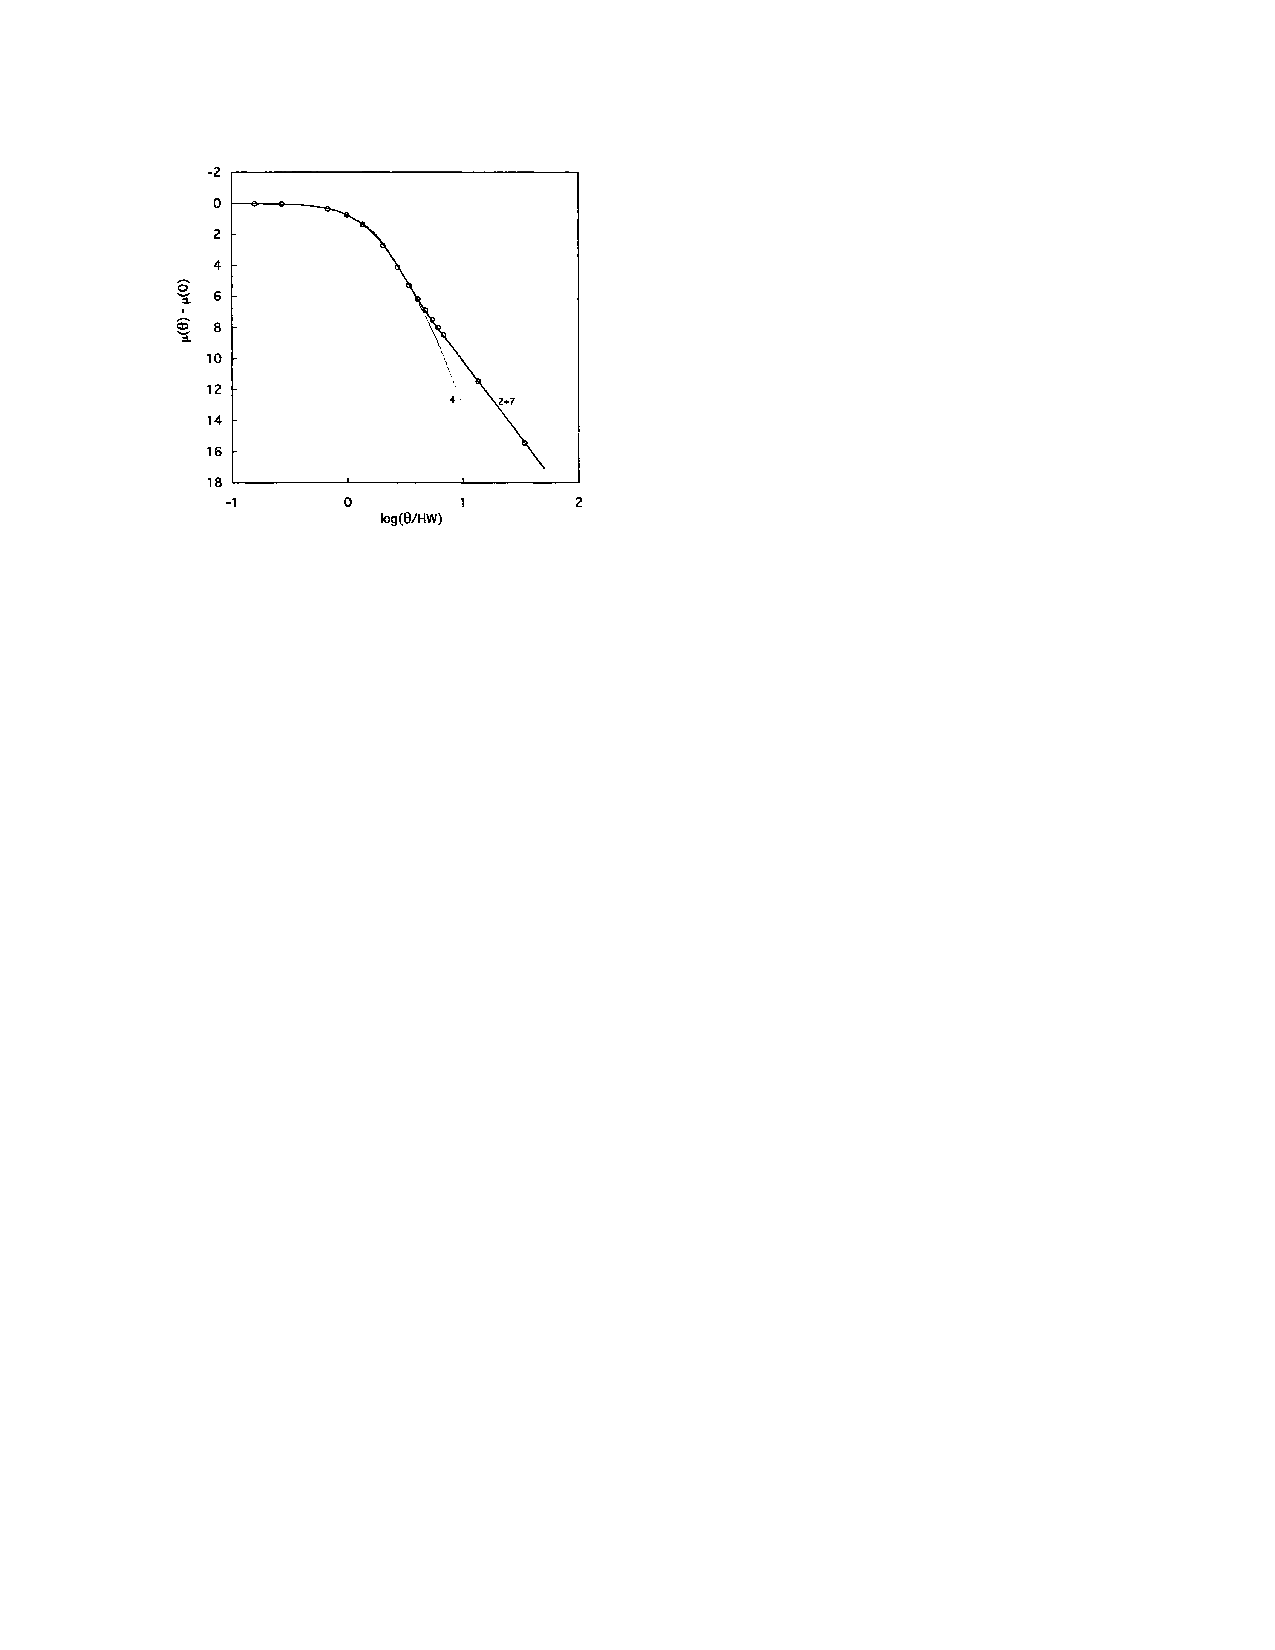
\includegraphics{figuras/PSFRacine}
	\caption[Ajuste de perfil de Moffat ao modelo de PSF de Kolmogorov]
	{Ajuste de perfil de Moffat (linhas sólidas) ao modelo de PSF de Kolmogorov
	(círculos abertos). A linha fina, é um perfil de Moffat com $\beta\!=\!4$, e a
	linha espessa é a soma de dois perfis de Moffat, com $\beta\!=\!7$ ($80\,\%$
	do fluxo) e $\beta\!=\!2$ ($20\,\%$ do fluxo). Retirado de \citet{Racine1996}.}
	\label{fig:PSFRacine}
\end{figure}

Se a PSF é constante em todo o campo, seu efeito na imagem pode ser calculado
como a convolução entre a imagem da PSF e a imagem original. Isto tem um custo
computacional extremamente elevado, especialmente quando se utiliza algum
procedimento iterativo como um ajuste de modelo. Uma convolução, em cálculo
numérico, significa calcular uma integral em duas dimensões para cada {\em
pixel}, ou seja, escala com $\mathcal{O}(n^2)$. Um truque bastante comum é
utilizar transformadas de Fourier para simplificar este cálculo e transformá-lo
num algoritmo que escala com $\mathcal{O}(n \log n)$. Se $I$ é a imagem original
e $I^\mathrm{PSF}$ a imagem da PSF, a imagem final $I^\ast$ é dada por
\begin{equation*}
I^\ast = I \otimes I^\mathrm{PSF}.
\end{equation*}
Aplicando a transformada de Fourier,
\begin{align*}
\mathcal{F}\{I^\ast\} &= \mathcal{F}\{I \otimes
I^\mathrm{PSF}\} \\
&= \mathcal{F}\{I\} \cdot \mathcal{F}\{I^\mathrm{PSF}\},
\end{align*}
ou seja, troca-se uma convolução por uma multiplicação. Para obter a imagem
final, basta aplicar a transformada de Fourier inversa sobre o produto. A
transformada de Fourier da PSF é sempre a mesma, logo a cada iteração apenas
duas integrais numéricas em duas dimensões são necessárias: a transformada da
imagem original e a transformada inversa para a imagem final. O ganho é tão
significativo que praticamente todos os programas de ajuste de imagens
astronômicas utilizam transformadas de Fourier para convoluir a imagem.


%***************************************************************%
%                                                               %
%                       PSF do CALIFA                           %
%                                                               %
%***************************************************************%
\section{Medindo a PSF}
\label{sec:psf:medida}

Para determinar as caraterísticas da PSF, idealmente é preciso observar um
objeto pontual brilhante, em várias regiões do campo do detector, e com as
mesmas condições atmosféricas que as observações. Raramente estas condições são
preenchidas, mesmo para fotometria CCD com campos muito grandes. Assim, conhecer
a PSF em instrumentos IFU não é uma tarefa trivial. Ainda há o fato de que as
imagens são reconstruídas através de técnicas de {\em dithering} (ver Seção
\ref{sec:ifs:instrumentacao}), e, dependendo o algoritmo utilizado, a PSF pode
nem sequer ser analítica. Entretanto, é preciso de algum modo obter uma
aproximação da forma da PSF para poder modelar a morfologia de uma galáxia
(Capítulo \ref{sec:morph}), especialmente o seu bojo. O procedimento descrito a
seguir é mais um esforço para entender a PSF e poder realizar a decomposição
morfológica do que um estudo aprofundado sobre o tema.

Para o CALIFA, observar campos estelares para caracterizar a PSF significaria a
redução no número de galáxias na amostra final do {\em survey}. Dadas as
restrições de tempo de telescópio e de significância estatística da amostra,
além do fato de a PSF não ser fundamental para os casos científicos alvo do {\em
survey}, estas observações não foram realizadas. Porém, sendo um {\em survey}
espectroscópico, o CALIFA necessita de observações de ``velas padrão'' para
calibrar o fluxo das galáxias. Foram observadas 45 estrelas para este fim, as
quais foram reaproveitadas aqui para análise da PSF.
Estas estrelas se encontram no centro no campo de observação do instrumento, com
um tempo de exposição muito menor do que o das galáxias ($120\,\mathrm{s}$
contra $900\,\mathrm{s}$). Esta amostra foi denominada ``estrelas de
calibração''. Alternativamente, pode-se procurar estrelas que apareçam na frente
das galáxias do {\em survey}. Neste caso a vantagem é que as estrelas têm o
mesmo tempo de exposição das galáxias, e são observadas nas mesmas condições
atmosféricas. Porém, não se encontram estas estrelas intrometidas em todos os
cubos, logo obter uma PSF para cada um deles está descartado. Outro problema em
potencial é que elas em geral, por construção do {\em survey}, são fracas e se
localizam na periferia do campo de observação. Esta amostra foi denominada
``estrelas de campo'', com 9 estrelas suficientemente brilhantes escolhidas em
cubos de galáxias {\em early type}. As duas amostras de estrelas reaproveitadas
foram usadas para caracterizar a PSF do CALIFA com o procedimento descrito a
seguir.

\begin{figure}
	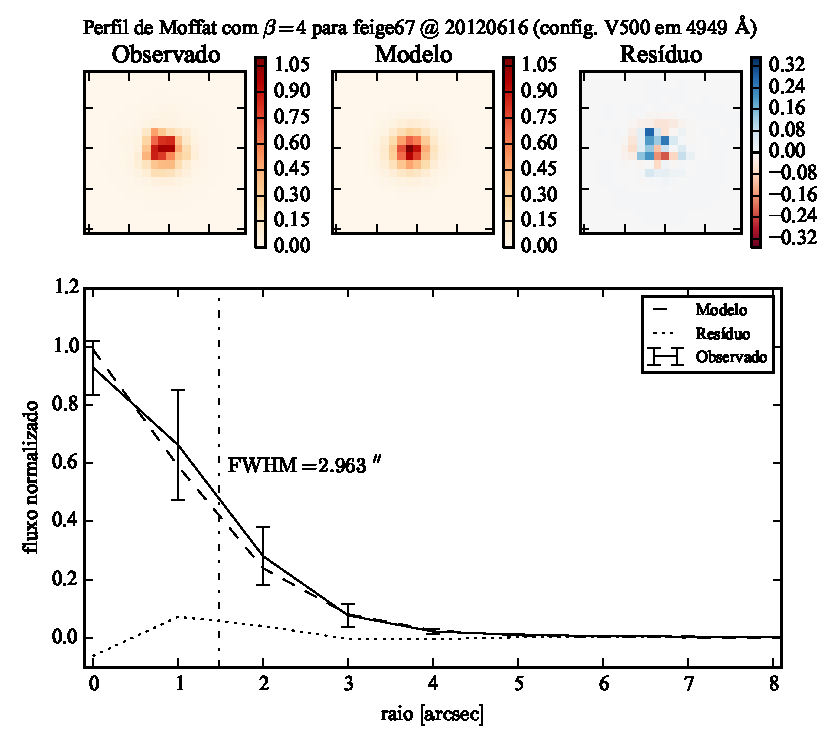
\includegraphics{figuras/PSFMoffatBeta4_exemplo}
	\caption[Exemplo de ajuste de PSF para estrela de calibração]
	{Exemplo de ajuste de PSF para a estrela de calibração Feige67, observada em
	16/06/2012, com a configuração V500. O modelo ajustado foi um perfil de
	Moffat elipsoidal com $\beta=4$. Nos painéis superiores estão imagens do fluxo
	observado numa caixa de $400\,\angstrom$ centrada em $4949\,\angstrom$,
	do modelo ajustado e do resíduo do ajuste. No painel inferior mostra-se o
	perfil de brilho radial médio: observado (linha sólida, onde as barras de erro
	são $\pm 1\,\sigma$ da média), modelo (linha tracejada, e a linha traço--ponto
	marca a largura a meia altura $\mathrm{FWHM}=2,963\,\arcs$) e resíduo (linha
	pontilhada).}
	\label{fig:PSFExemplo}
\end{figure}

O modelo utilizado foi um perfil de Moffat 2-D elipsoidal, com $\beta\!=\!4$,
conforme visto na Seção \ref{sec:psf:teoria}. Os cubos foram combinados em
caixas de $400\,\angstrom$ de largura, gerando 10 imagens de fluxo e incerteza
para cada estrela. Estas imagens foram ajustadas aos modelos através de um
programa desenvolvido utilizando a biblioteca
\textsc{python-imfit}\footnote{\textsc{python-imfit} é uma biblioteca baseada no
programa \textsc{imfit} de \citet{Erwin2015}, a mesma utilizada no programa de
decomposição morfológica, ver Seção \ref{sec:morph:comp:depLambda}.}. O
resultado do ajuste são os parâmetros do perfil de Moffat e a estatística
$\chi^2$ do melhor modelo.
A Figura \ref{fig:PSFExemplo} ilustra o ajuste feito para uma estrela de
calibração, numa faixa espectral próxima a $5000\,\angstrom$.

% FIXME: A integral disso nao deveria ser =1? Entao essa escala y nao quer dizer
% nada.

\begin{figure}
	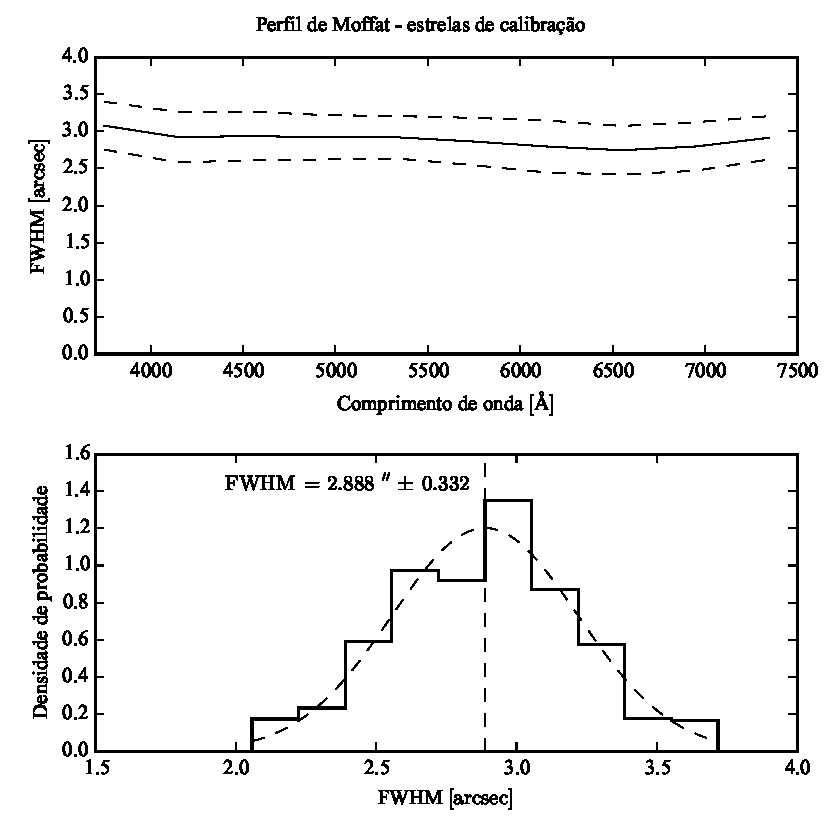
\includegraphics{figuras/PSFMoffatBeta4_calib}
	\caption[PSF do CALIFA -- estrelas de calibração]
	{PSF do CALIFA modelada como um perfil de Moffat com $\beta=4$, utilizando 45
	estrelas de calibração. {\em Acima}: FWHM da PSF em função do comprimento de
	onda (caixas de $400\,\angstrom$). As linhas tracejadas indicam a distribuição
	em $1\ \sigma$. {\em Abaixo}: Histograma da FWHM da PSF, ponderado pela
	verossimilhança do modelo em todos os comprimento de onda de todas as estrelas,
	com $\mathrm{FWHM}=2,888 \pm 0,332\,\arcs$.}
	\label{fig:PSFCalib}
\end{figure}

Este procedimento foi realizado para as 45 estrelas de calibração, e o resultado
pode ser visto na Figura \ref{fig:PSFCalib}. Praticamente não há dependência da
PSF com o comprimento de onda, como se pode verificar no painel superior da
figura. Na mesma figura, no painel inferior, mostra-se um histograma ponderado
pela verossimilhança ($\operatorname{e}^{-\chi^2/2}$) de todos os ajustes (todas
as estrelas em todas as caixas de comprimento de onda). Desta distribuição
obtém-se uma largura a meia altura média de $\mathrm{FWHM} = 2,888 \pm
0,332\,\arcs$. A elipticidade ($\epsilon = 1 - b/a$) média encontrada é de
$\epsilon = 0,097 \pm 0,065$, ou seja, a PSF é praticamente circular. A
incerteza nos dois casos representa o desvio padrão ($1\,\sigma$) da média
ponderada. O mesmo vale para todas as incertezas obtidas no resto desta seção.

\begin{figure}
	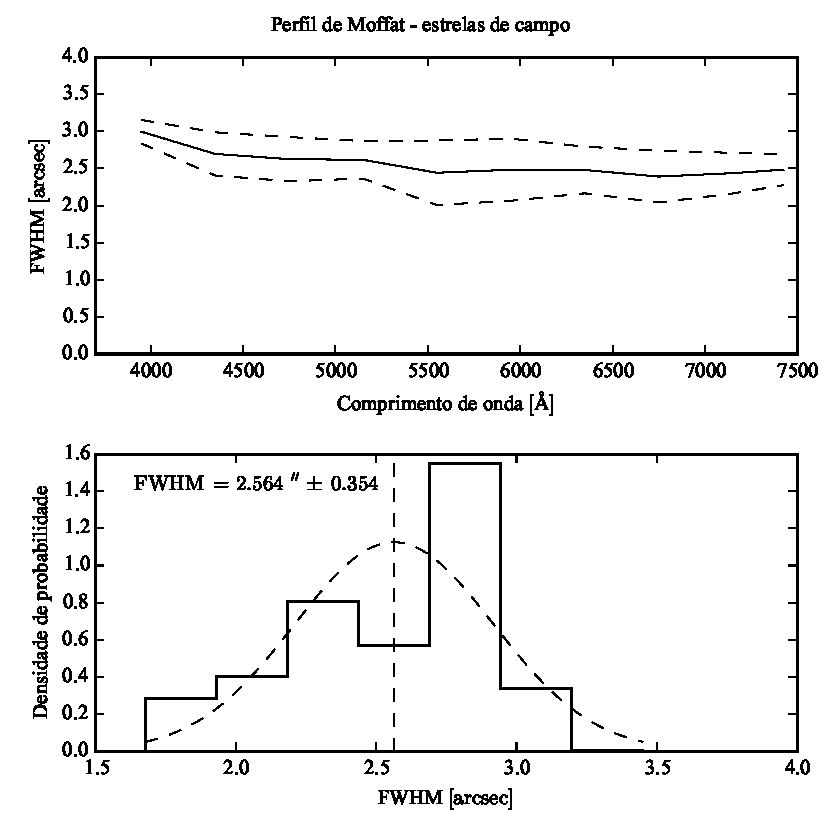
\includegraphics{figuras/PSFMoffatBeta4_field}
	\caption[PSF do CALIFA -- estrelas de campo]
	{PSF do CALIFA modelada como um perfil de Moffat com $\beta=4$, utilizando 9
	estrelas de campo, na frente das galáxias observadas. {\em Acima}: FWHM da PSF
	em função do comprimento de onda (caixas de $400\,\angstrom$). As linhas
	tracejadas indicam a distribuição em $1\ \sigma$. {\em Abaixo}: Histograma da
	FWHM da PSF, ponderada pela verossimilhança do modelo em todos os comprimentos
	de onda de todas as estrelas, com $\mathrm{FWHM}=2,564 \pm 0,354\,\arcs$.}
	\label{fig:PSFField}
\end{figure}

O mesmo procedimento foi realizado para as 9 estrelas de campo, presentes nos
cubos de galáxias do {\em survey} e normalmente mascarados por não serem de
interesse no estudo do espectro das galáxias. As estrelas desta amostra estão na
frente de galáxias com simetria axial (elípticas e S0). Dado um cubo de uma
galáxia, recortaram-se 7 {\em spaxels} ao redor da estrela, gerando dois cubos:
um da galáxia, com a estrela mascarada, e outro da estrela. Neste ponto o cubo da
estrela ainda está contaminado pela luz da galáxia. Então, considerando que a
galáxia tem simetria axial, calculou-se um perfil de brilho radial médio da
galáxia (ver Seção \ref{sec:pycasso:Pycasso}, Figura \ref{fig:radprofIdade}),
para cada comprimento de onda. Com este perfil, é possível estimar quanto a
galáxia está contribuindo para a luz de cada {\em spaxel} do cubo da estrela,
pois a distância de cada {\em spaxel} ao centro da galáxia é conhecido. Criou-se
assim um cubo de ``luz de fundo'' para a mesma região que contém a estrela.
Subtraindo o cubo de fundo do cubo da estrela, obteve-se um cubo com apenas a
luz proveniente da estrela. Este cubo foi então analisado da mesma forma que os
cubos de estrelas de calibração, com os resultados mostrados na Figura
\ref{fig:PSFField}. Da mesma forma, não há dependência da FWHM da PSF com o
comprimento de onda, com $\mathrm{FWHM}=2,564 \pm 0,354\,\arcs$ e elipticidade
$\epsilon=0,093 \pm 0,059$.

% FIXME: Natalia - Parece mais assimetrica que a outra. Nao seria melhor
% reportar mediana e percentis para mostrar se eh muito assimetrica ou nao? E
% isso iria influenciar todo o paragrafo segunte tambem.

Há uma diferença considerável no valor obtido para a FWHM da PSF nos dois casos,
embora eles estejam a cerca de $1\,\sigma$ de separação. Isto poderia indicar
uma diferença sistemática entre a PSF das estrelas de calibração e a PSF das
estrelas de campo. Todavia, observando atentamente o histograma de FWHM das
estrelas de campo (painel inferior da Figura \ref{fig:PSFField}), pode-se notar
que o valor mais frequente da distribuição (moda) é aproximadamente
$2,8\,\arcs$, muito próximo do valor obtido para as estrelas de calibração. A
distribuição se desvia de uma gaussiana, com a média ponderada da FWHM da PSF
das estrelas de campo menor do que o valor mais frequente. Isto, aliado ao fato
de que o tamanho da amostra de estrelas de calibração (45) é maior do que o das
estrelas de campo (9), fez com que se escolhesse a medida da primeira amostra
como a mais confiável.

Já com os valores de elipticidade ($\epsilon$) obtidos nos dois casos, os
semieixos maior e menor da FWHM estão dentro da faixa de $1\,\sigma$ um do
outro. E, em ambos os casos, $\epsilon$ é muito próximo a zero, dentro da
incerteza. Levar a elipticidade em conta seria adicionar uma complexidade
desnecessária (e possivelmente artificial) ao modelo de PSF.

Assim, a PSF adotada neste trabalho é um perfil de Moffat com simetria axial,
$\beta\!=\!4$ e $\mathrm{FWHM}=2,9 \pm 0,3\,\arcs$. Este foi o mesmo
procedimento para fazer a caracterização da PSF publicada no DR2 do CALIFA
\citep{GarciaBenito2015}, mas com uma diferença. Naquele caso, ajustaram-se
tanto FWHM quanto $\beta$, obtendo-se $\mathrm{FWHM}=2,39 \pm 0,26\,\arcs$ e
$\beta=1,73 \pm 0,11$. A diferença está basicamente em qual região da PSF se
está interessado em modelar mais precisamente. Por uma questão geométrica, há
mais {\em pixels} longe do centro do perfil, o que acaba causando mais peso
destas regiões periféricas no modelo escolhido pelo ajuste (ver as barras de
erro cada vez menores com a distância, na Figura \ref{fig:PSFExemplo}, que são a
grosso modo inversamente proporcionais ao peso). Porém, na maioria destes {\em
pixels} periféricos o fluxo proveniente da estrela já está submerso no ruído,
achatando o perfil (isto é, diminuindo $\beta$). O ajuste resultante é então
pior nas regiões centrais, com peso menor.
No caso do ajuste morfológico de uma galáxia, em particular utilizando um perfil
concentrado como o de Sérsic para o bojo, requer uma forma precisa da PSF nas
regiões centrais. Qualquer erro sistemático na forma da PSF pode causar
problemas na determinação dos parâmetros morfológicos do bojo.
Desta forma, optou-se por refazer a análise da PSF para esta tese com $\beta$
fixo.

% FIXME: Rogério - Sugestões:
%
% * Com BLR pode ser um teste interessante.
% * Como tem duas PSF publicadas, qual a PSF do CALIFA?

% FIXME: Natalia - Em resumo, a PSF publicada está errada?
% Também, rever o comentário sobre barras de erro e pesos.

% End of this chapter

  
  % Testes da decomposição e efeitos da PSF
  %%%%%%%%%%%%%%%%%%%%%%%%%%%%%%%%%%%%%%%%%%%%%%%%%%%%%%%%%%%%%%%%%
% Tese de Doutorado / Dept Fisica, CFM, UFSC                    %
% Andre@UFSC - 2014                                             %
%%%%%%%%%%%%%%%%%%%%%%%%%%%%%%%%%%%%%%%%%%%%%%%%%%%%%%%%%%%%%%%%%

%:::::::::::::::::::::::::::::::::::::::::::::::::::::::::::::::%
%                                                               %
%                          Capítulo 6                           %
%                                                               %
%:::::::::::::::::::::::::::::::::::::::::::::::::::::::::::::::%

%***************************************************************%
%                                                               %
%         Testes da decomposição morfológica espectral          %
%                                                               %
%***************************************************************%

\chapter{Testes da decomposição morfológica espectral}
\label{sec:test}

O processo de fazer a decomposição morfológica em cubos de dados espectrais de
galáxias, tal que se toma imagens de fatias em comprimento de onda, é chamado
daqui em diante de decomposição morfológica espectral. Este processo resulta
numa sequência de modelos em função do comprimento de onda. Avaliando os modelos
como imagens, é póssível montar cubos de dados espectrais para as componentes do
modelo. Ou seja, com um modelo bojo e disco, a decomposição de um cubo de dados
de uma galáxia gera dois cubos, um para o bojo e outro para o disco.

De posse destes cubos de dados espectrais das componentes, pode-se começar a
ponderar o significado de um {\em spaxel} deste cubo. Instintivamente, espera-se
que ele se pareça a um {\em spaxel} da galáxia original. Mas, nada garante que
ele deva ser parecido com espectro algum, afinal o cubo espectral da componente
morfológica é resultado de um processo computacional bastante complexo.
Também, como se comentou na Seção \ref{sec:morph:comp:bd}, é preciso ter cuidado
ao interpretar o resultado de um ajuste de modelo empírico.
Isto é ainda mais importante em casos onde se faz este ajuste de forma
automatizada, sem inspecionar cada imagem e seus modelos de forma individual,
como é o caso da decomposição morfológica espectral.

O próximo Capítulo trata da decomposição morfológica espectral de cubos de dados
do CALIFA. A fim de determinar se o método funciona, foi construído um modelo de
galáxia simples, com parâmetros morfológicos e espectros das componentes
conhecidos. A decomposição foi aplicada a esta galáxia sintética, com o
resultado apresentado a seguir.

%***************************************************************%
%                                                               %
%                   Construindo uma galáxia                     %
%                                                               %
%***************************************************************%
\section{Construindo uma galáxia}

Não é objetivo deste exercício modelar uma galáxia realista. Os parâmetros foram
escolhidos apenas para que o modelo que se assemelhe a uma galáxia real, sem
qualquer necessidade de ser fisicamente possível tal galáxia existir. O modelo
utilizado foi um bojo com uma lei de Sérsic e um disco com uma lei exponencial
(ver Seção \ref{sec:morph:comp:bd}), cada componente com um perfil elipsoidal
distinto dado por uma elipsidade ($\epsilon = 1 - b/a$, onde $a$ e $b$ são os
semieixos maior e menor) e um ângulo de posição (P.A.) medido em sentido
anti-horário a partir do eixo horizontal. Os parâmetros, do modelo são os
seguintes:

\begin{tabular}{ l  r | l  r }
  \hline
  \multicolumn{4}{c}{Modelo original} \\
  \multicolumn{2}{c}{Bojo} & \multicolumn{2}{c}{Disco} \\
  \hline
  $I_e$ & $2,0$ & $I_0$ & $1.0$ \\
  $r_e$ & $5,0\,\arcs$ & $h$ & $15.0\,\arcs$ \\
  $n$ & $4$ & & \\
  $\mathrm{P.A.}$ & $60^\circ$ & $\mathrm{P.A.}$ & $45^\circ$ \\
  $\epsilon$ & $0,1$ & $\epsilon$ & $0,1$ \\
  \hline
\end{tabular}

\begin{figure}
	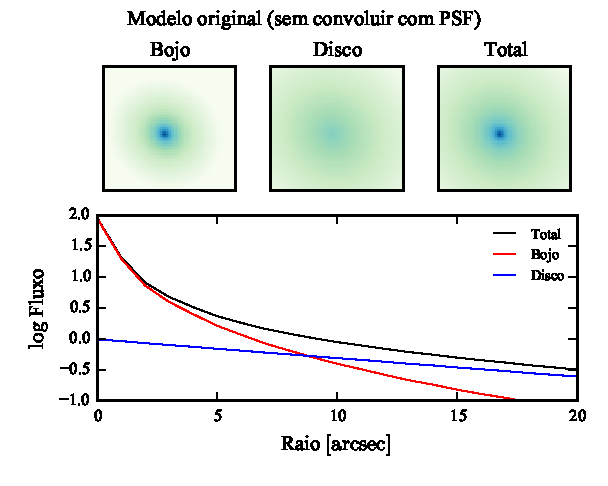
\includegraphics{figuras/simulation_initmodel}
	\caption[Modelo morfológico inicial da galáxia sintética.]
	{Modelo morfológico da galáxia sintética utilizada para testar a decomposição
	morfológica espectral. A este modelo ainda não foi aplicada a convolução com a
	PSF. Acima, a imagem referente às componentes bojo e disco, e total (bojo +
	disco). Abaixo, o perfil radial de brilho, calculado em isofotas da imagem
	total.}
	\label{fig:testInitmodel}
\end{figure}

Este modelo original, mostrado na Figura \ref{fig:testInitmodel}, descreve o
brilho superficial da galáxia no comprimento de onda de normalização escolhido,
$5635\,\angstrom$.

\begin{figure}
	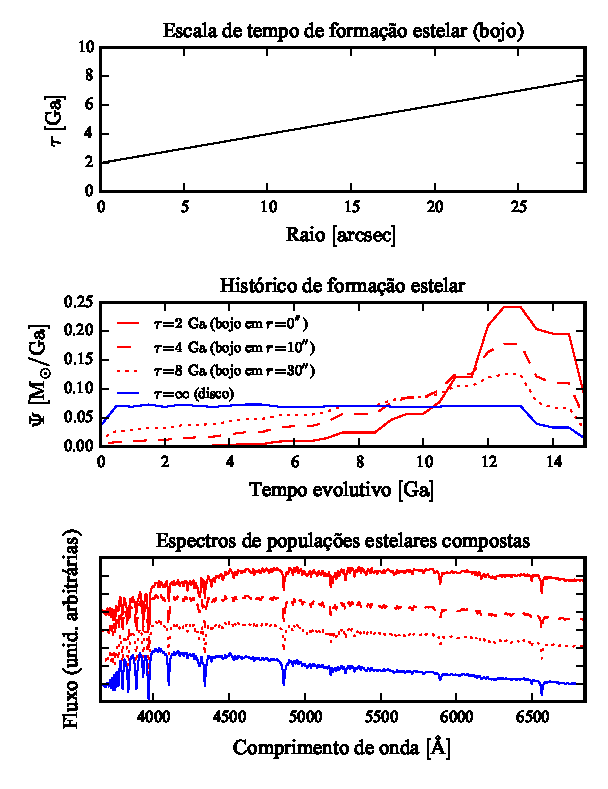
\includegraphics{figuras/simulation_popmodel}
	\caption[Modelos de populações estelares da galáxia sintética.]
	{Modelos de populações estelares das componentes bojo (em vemelho)
	e disco (em azul) da galáxia sintética. No painel superior, a dependência
	espacial do tempo de escala do decaimento, $\tau$, da SFR do bojo. No painel
	central taxas de formação estelar (SFR), modelados como $\Psi(t) = A \exp
	(t/\tau)$. A SFR do disco é constante, com $\tau\to\infty$. Abaixo, os
	espectros resultantes, utilizando a base de Granada.}
	\label{fig:testPopmodel}
\end{figure}

Para transformar este modelo num cubo de dados espectral, deve-se estendê-lo na
direção de comprimento de onda. Utilizando espectros de populações estelares
simples (SSP) de uma base e históricos de formação estelar (SFH) sintéticos
para cada componente, obteve-se espectros para cada {\em pixel} da galáxia. Neste
teste, o SFH do disco é sempre o mesmo, independente da posição na componente.
Isto significa que todos os espectros do disco têm a mesma forma, modulados pela
distribuição espacial de briho dado pelo modelo morfológico (Figura
\ref{fig:testInitmodel}). Já o SFH do bojo varia com a posição, ou seja, os
espectros variam tanto em forma quanto em intensidade. A forma exata dos SFH do
bojo e do disco não é relevante, basta que representem populações
suficientemente diferentes uma da outra. O modelo de populações é mostrado na
Figura \ref{fig:testPopmodel}.

Escolheu-se modelar o SFH do bojo como um surto de decaimento exponencial de
formação estelar, com a taxa de formação estelar em função do tempo (SFR)
sintética dada por $\Psi(t) = A \exp (t/\tau)$, normalizada de tal forma que
$\int \Psi(t)\,\mathrm{d}t = 1\,\mathrm{M}_\odot$. O SFH do disco consiste numa
SFR constante. A escala de tempo de decaimento $\tau$ tem a sua dependência
espacial, no bojo, dada pela lei linear $\tau = \tau_0 + \alpha r$, onde
$\tau_0$ é o seu valor no núcleo da galáxia e $\alpha$ o seu gradiente. Foram
escolhidos $\tau_0 = 2\,\mathrm{Ga}$ e $\alpha = 0,2\,\mathrm{Ga} / \arcs$, com
um $\tau$ resultante mostrado no o painel superior da Figura
\ref{fig:testPopmodel}. Para o disco, a SFR constante é obtida com
$\tau\to\infty$. Estas SFR sintéticas foram discretizadas para aplicar a uma
base de modelos de SSP. A base utilizada foi a de Granada, explicada na Seção
\ref{sec:ifs:starlight}. A SFR do bojo e do disco estão mostrados no painel
central da mesma figura, respectivamente em vermelho e azul. A forma das SFR
foge um pouco de uma exponencial devido ao fato de a base de modelos não ser
homogeneamente espaçada em idade. Os espectros finais são obtidos somando os
espectros da base, com o peso dado pelo vetor de população obtido das SFR
sintéticas. O painel inferior da Figura \ref{fig:testPopmodel} mostra os
espectros do bojo para $r = 0$, $10$ e $30\,\arcs$ com o mesmo código de cores
das SFR. O espectro do bojo tem um aspecto de populações velhas no centro da
galáxia ($\tau = 2\,\mathrm{Ga}$), e vai ficando cada vez mais jovem a medida
que se afasta. O espectro do disco é sempre mais jovem do que o do bojo.

Nenhuma outra propriedade física foi modelada. Poderia-se adicionar poeira, por
exemplo, mas isto não faria diferença no teste. O importante aqui é que bojo e
disco tenham espectros diferentes, e que os espectros possam variar de forma com
a posição. Por outro lado, a cinemática mereceria um teste dedicado. Modelar (e
levar em conta no ajuste morfológico) o efeito da cinemática não é uma tarefa
trivial, já que bojos e discos têm cinemáticas completamente distintas. Este é
certamente um problema que deve ser visitado no futuro.

Multiplicando a imagem do modelo pelo conjunto de espectros de cada componente,
obteve-se um cubo de dados espectral para bojo e disco. Para obter o cubo da
galáxia sintética, somou-se os dois componentes, convoluiu-se com a PSF de
$\mathrm{FWHM} = 2,9\,\arcs$, e adicionou-se ruído gaussiano de $5\%$ (para um
sinal--ruído de $20$). Para deixar o cubo em dimensões parecidas à do CALIFA, os
{\em spaxels} a uma distância $r > 32\,\arcs$ foram mascarados, como aparece nos
painéis superiores da Figura \ref{fig:testFitmodel}, descrita na próxima seção.

%***************************************************************%
%                                                               %
%               Decompondo a galáxia sintética                  %
%                                                               %
%***************************************************************%
\section{Decompondo a galáxia sintética}

O algoritmo da decomposição morfológica espectral é tratado em detalhes no
Capítulo \ref{sec:Decomp}, sendo descrito apenas superficialmente nesta seção.

\begin{figure}
	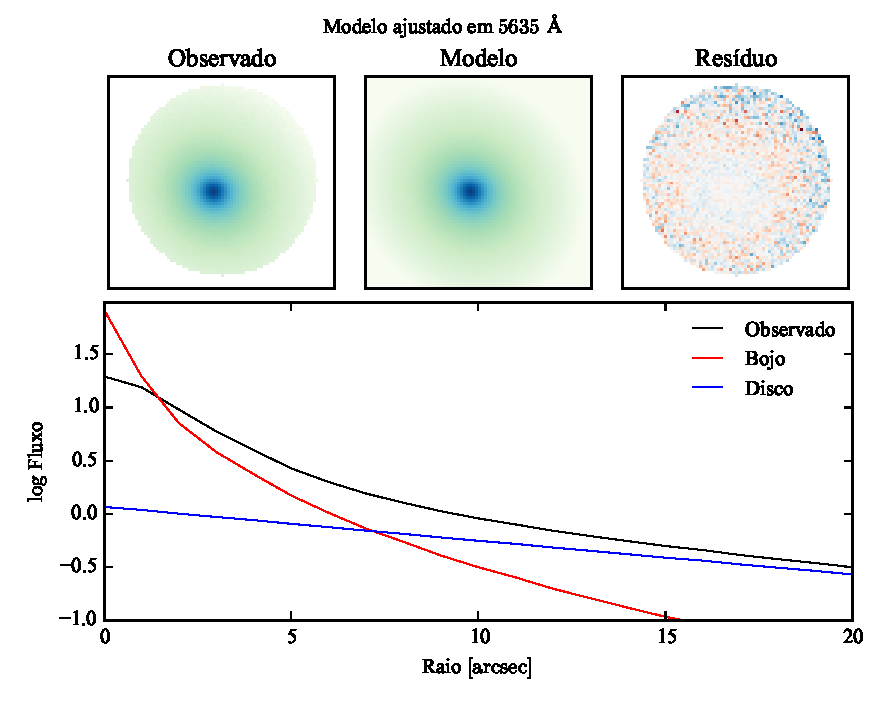
\includegraphics{figuras/simulation_fitmodel}
	\caption[Modelo morfológico inicial do ajuste da galáxia sintética.]
	{Modelo morfológico ajustado à galáxia sintética em $5635\,\angstrom$
	utilizando o algoritmo DE. A imagem de resíduo é a diferença entre
	observado e modelo, nos painéis superiores. O perfil radial de brilho, no
	painel inferior, pode ser comparado com o da Figura \ref{fig:testInitmodel}.
	Este modelo foi usado como valor inicial na decomposição morfológica
	espectral.}
	\label{fig:testFitmodel}
\end{figure}

Como o objetivo é fazer a decomposição $\lambda$-a-$\lambda$, o algoritmo
escolhido foi o de LM (Seção \ref{sec:morph:comp:ajuste}). Ele pode ser
extremamente rápido, mas requer um bom modelo inicial. Então, o primeiro passo
na decomposição é encontrar um modelo com valores aproximado das propriedades
das componentes. Neste caso, pode-se utilizar um algorimo mais complexo, como o
DE, que requer apenas uma faixa de valores para os parâmetros do modelo.
A decomposição foi feita com a mesma PSF utilizada para criar o cubo,
$\mathrm{FWHM} = 2,9\,\arcs$. Na Seção \ref{sec:test:psf} discute-se o que
acontece quando se utiliza uma PSF diferente da ideal.

A Figura \ref{fig:testFitmodel} mostra o modelo ajustado inicial. O ajuste
foi feito numa faixa de $90\,\angstrom$ ao redor de $5635\,\angstrom$ (a
mesma utilizada para normalizar os espectros antes de rodar o \starlight).
O ajuste foi suficientemente bom, próximo ao modelo original (comparar com a
Figura \ref{fig:testInitmodel}). Os parâmetros do modelo são os seguintes: 

\begin{tabular}{ l  r | l  r }
  \hline
  \multicolumn{4}{c}{Ajuste inicial} \\
  \multicolumn{2}{c}{Bojo} & \multicolumn{2}{c}{Disco} \\
  \hline
  $I_e$ & $3,0$ & $I_0$ & $1,2$ \\
  $r_e$ & $3,9\,\arcs$ & $h$ & $14,3\,\arcs$ \\
  $n$ & $3,4$ & & \\
  $\mathrm{P.A.}$ & $60,3^\circ$ & $\mathrm{P.A.}$ & $46,5^\circ$ \\
  $\epsilon$ & $0,1$ & $\epsilon$ & $0,1$ \\
  \hline
\end{tabular}

Este ajuste não precisa ser perfeito, ele será refinado no primeiro passo do
ajuste espectral. Espera-se que os  parâmetros mofológicos variem com o
comprimento de onda, logo o valor inicial deve variar de acordo. O cubo
espectral é então quebrado em caixas de $200\,\angstrom$, cada fatia sendo
somada em comprimento de onda, formando várias imagens. Cada imagem é ajustada,
agora com algoritmo de LM, e os parâmetros são, independentemente, ajustados a
uma reta em função do comprimento de onda. Estas retas, uma para cada parâmetro,
formam os modelos iniciais para o segundo passo, a decomposição
$\lambda$-a-$\lambda$ do cubo de dados espectral da galáxia sintética.

\begin{figure}
	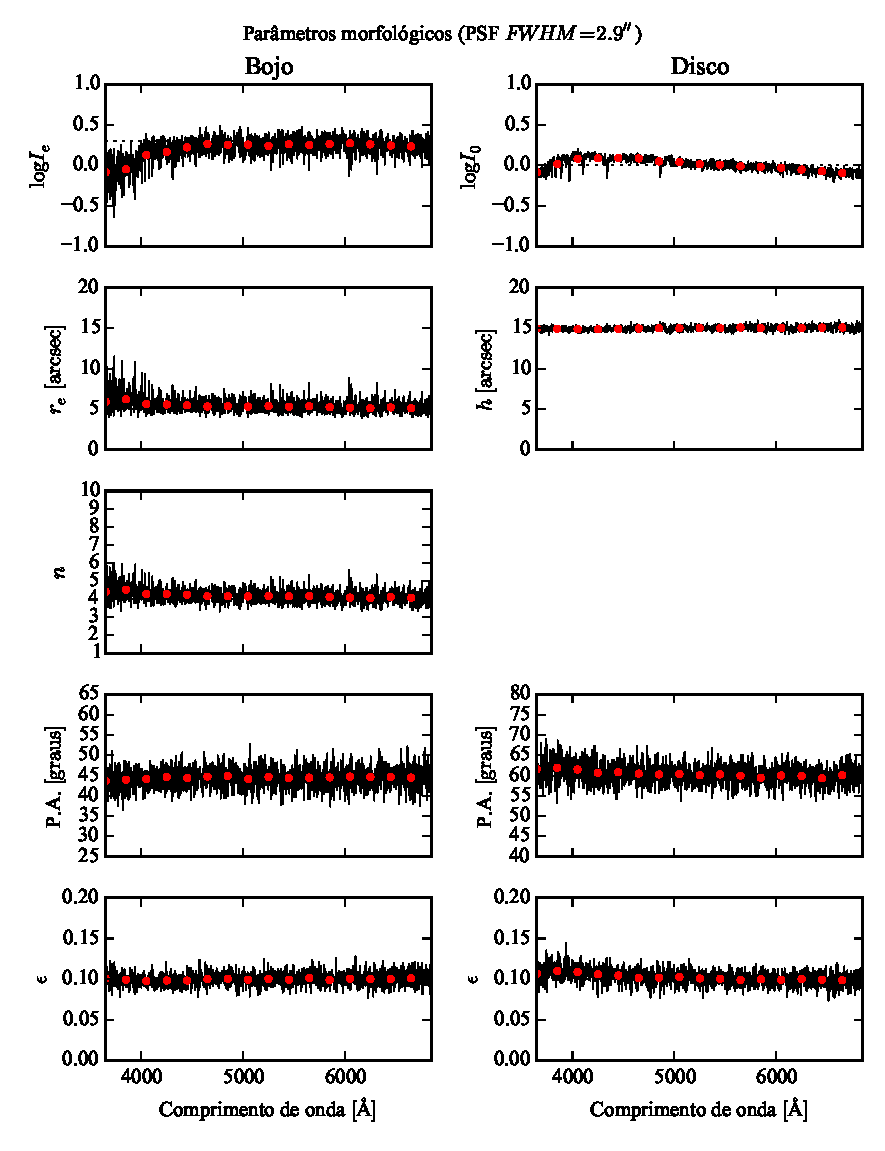
\includegraphics{figuras/simulation_fitparams}
	\caption[Parâmetos morfológicos da galáxia sintética.]
	{Parâmetos morfológicos da galáxia sintética, em função do comprimento de
	onda. Pontos vermelhos indicam o ajuste feito em caixas de $200\,\angstrom$, e
	as linhas indicam o ajuste feito $\lambda$-a-$\lambda$. Linhas pontilhadas,
	que praticamente não aparecem por trás dos ajustes, são os parâmetros
	originais. Os painéis à esquerda são referentes ao bojo, e os à direita ao
	disco. Ajuste feito com uma PSF de $\mathrm{FWHM} = 2,9\,\arcs$.
	}
	\label{fig:testFitParams}
\end{figure}

Os parâmetros morfológicos ajustados, em função do comprimento de onda, são
mostrados na Figura \ref{fig:testFitParams}. Os ajustes individuais dos
parâmetros, $\lambda$-a-$\lambda$ (linhas pretas), não se afastam muito dos
parâmetros iniciais (pontos vermelhos), e concordam bem com o modelo original
(linhas pontilhadas), praticamente escondidas atrás das linhas de ajuste na
maioria dos gráficos. Os parâmetros $r_e$ e $n$, do bojo, parecem crescer um
pouco na região abaixo de $4000\,\angstrom$, o que pode indicar uma dependência
destes valores com as características da população estelar do bojo. O ajuste do
disco, por outro lado, é praticamente constante em comprimento de onda.
os parâmetros morfológicos médios, ponderados pela verossimilhança do ajuste,
são:

\begin{tabular}{ l  r | l  r }
  \hline
  \multicolumn{4}{c}{Ajuste espectral médio} \\
  \multicolumn{2}{c}{Bojo} & \multicolumn{2}{c}{Disco} \\
  \hline
  $r_e$ & $5,498 \pm 0.876\,\arcs$ & $h$ & $14,974 \pm 0,268\,\arcs$ \\
  $n$ & $4,206 \pm 0,389$ & & \\
  $\mathrm{P.A.}$ & $60,384 \pm 2,438^\circ$ & $\mathrm{P.A.}$ & $44,467 \pm
  2,452^\circ$ \\
  $\epsilon$ & $0,102 \pm 0,009$ & $\epsilon$ & $0,100 \pm 0,008$ \\
  \hline
\end{tabular}

Estes valores não necessariamente precisam ser iguais aos do modelo original.
Aquele foi usado para definir o modelo em $5635\,\angstrom$, e se a média
espectral se desvia dele, claramente é devido à dependência dos parâmetros
morfológicos com o comprimento de onda. Isto é, se a decomposição realmente
encontra os cubos espectrais do bojo e do disco. É preciso examinar os espectros
ajustados.

\begin{figure}
	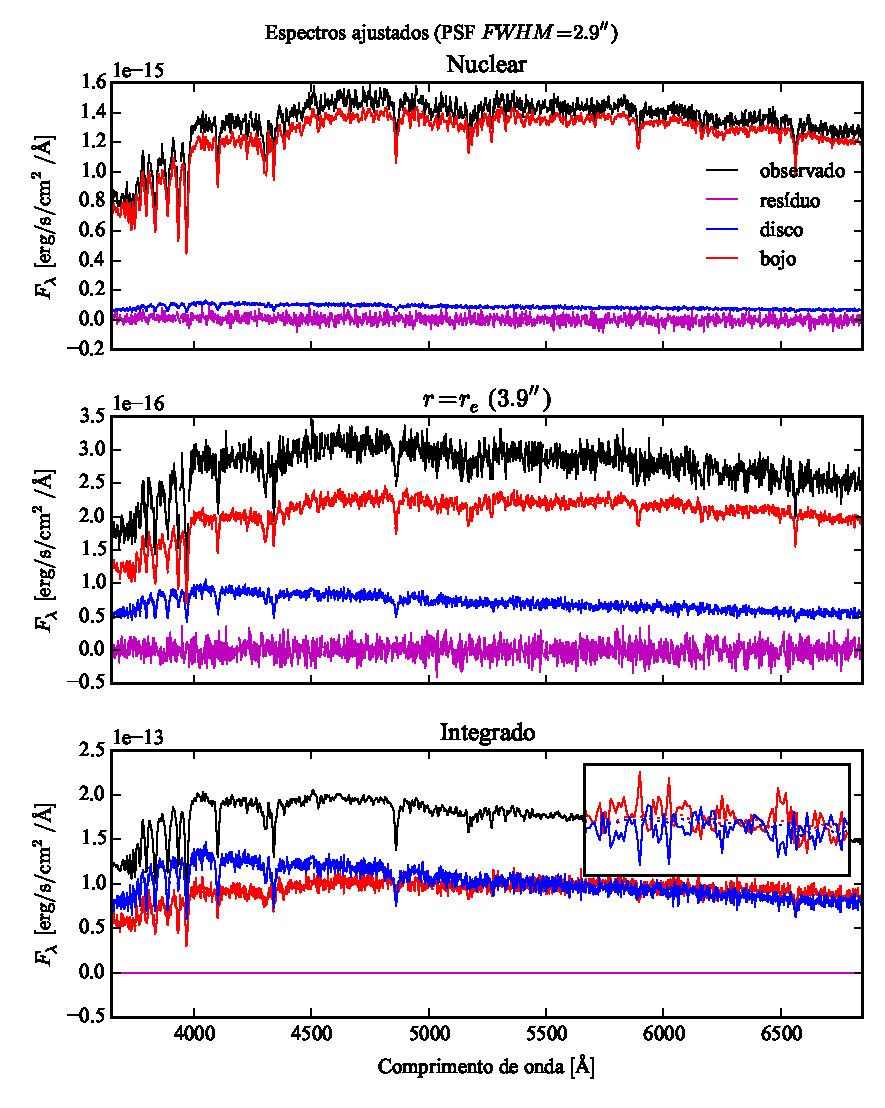
\includegraphics{figuras/simulation_spectra}
	\caption[Espectros ajustados à galáxia sintética.]
	{Espectros ajustados à galáxia sintética. Em preto o espectro observado, em
	vermelho o bojo, em azul o disco, e em magenta o resíduo. Os
	espectros dos componentes originais são as linhas pontilhadas, praticamente
	cobertas pelos ajustes. Os dois painéis superiores mostram a decomposição no
	{\em spaxels} nuclear e em $r=r_e$. Os espectros integrados espacialmente são
	mostrados no painel inferior.}
	\label{fig:testFitSpectra}
\end{figure}

A Figura \ref{fig:testFitSpectra} mostra os espectros em {\em spaxels}
escolhidos (núcleo, acima, e $r=r_e$, no centro), e os espectros integrados. Os
ajustes parecem muito bons, com os espectros originais (linhas pontilhadas)
praticamente indistinguíveis dos espectros ajustados (linhas contínuas). No caso
integrado, os espectros ajustados parecem ruidosos, mas o resíduo é praticamente
nulo. Isto quer dizer que aquela dispersão, que parece ruído, é na verdade
causada por degenerescência no ajuste. As variações nas duas componentes estão
anti-correlacionadas. Esta degenerescência precisa ser estudada mais a fundo no
futuro.

\begin{figure}
	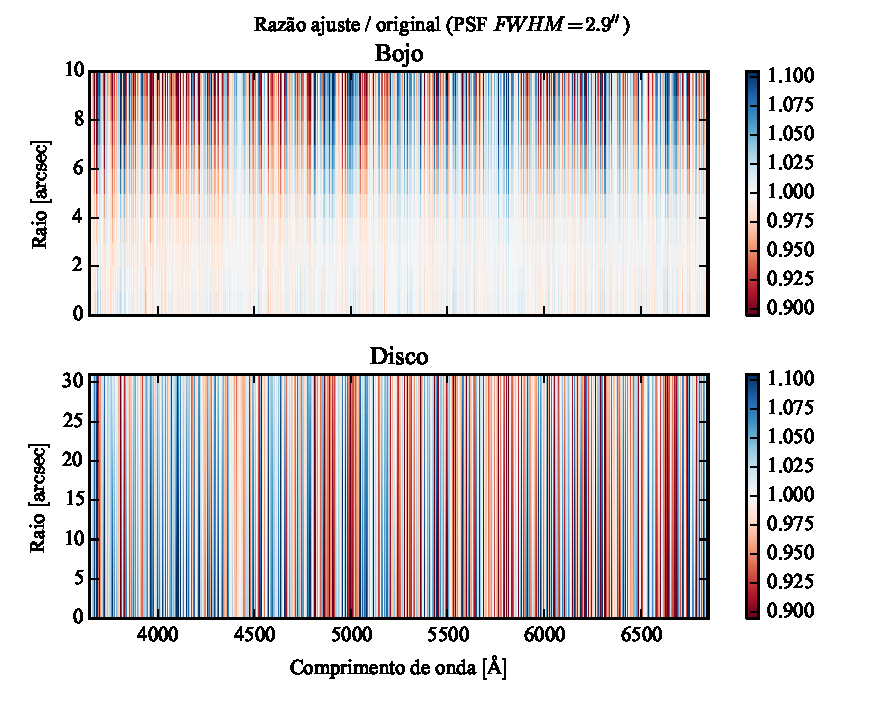
\includegraphics{figuras/simulation_error}
	\caption[Razão ajuste--original dos espectros ajustados à galáxia sintética.]
	{Razão ajuste--original média dos espectros ajustados à galáxia sintética, em
	função do comprimento de onda e da distância ao centro da galáxia, tomada em
	anéis de raio constante. Valores desviando de $1$ indicam erro no ajuste.
	Acima a razão para o bojo, e abaixo para o disco. A escala radial é
	diferente nos dois casos.}
	\label{fig:testFitError}
\end{figure}

Mesmo verificando visualmente que os espectros ajustados são parecidos com os
originais, é preciso quantificar a qualidade do ajuste. Calculando a média da
razão entre o ajuste e o original, obtém-se para o bojo um valor de $1,0021 \pm
0,0297$. Ou seja, o ajuste tem um desvio médio de menos de $1\%$, e um desvio
padrão da média de $3\%$. Para o disco a razão média é $0,9857 \pm 0.0466$, isto
é, um desvio médio de $1,5\%$, e um desvio padrão da média de $4,5\%$. O que
causa estes desvios? Deve-se explorar melhor a razão ajuste--original, para
determinar se existe algum efeito sistemático. A Figura \ref{fig:testFitError}
mostra a razão média em anéis de raio constante, para que seja possível fazer
uma imagem em duas dimensões. O ajuste do bojo, mostrado às esquerda, tem um
desvio menor no centro, e vai aumentando conforme se afasta do núcleo. O ajuste
do disco, à direita, parece não ter desvios espaciais significativos. Não há
também um gradiente espectral apreciável, isto é, uma cor, nas duas componentes.
Entretanto, ambas mostram o surgimento de ``linhas espectrais artificiais'', que
parecem estar anti-correlacionadas, conforme foi visto nos espectros integrados.

Em linhas gerais, o resutado do teste é promissor. Idealmente, é necessário
testar todas as configurações possíveis de morfologia, para mapear em quais
delas a decomposição espectral é válida. Mas, é preciso lembrar que o modelo
morfológico tem 7 parâmetros livres. Se cada um deles puder tomar $n$ valores
diferentes, a quantidade de modelos a serem testados é $n^7$. Com somente 4
valores por parâmetro, são mais de 16 mil modelos possíveis, o que, com cada
decomposição levando cerca de 5 minutos em um computador de 24 núcleos, leva
mais de 50 dias, sem contar o tempo necessário para análise dos resultados. Isso
sem incluir populações estelares variáveis, e diferentes PSFs (ver a Seção
seguinte). Esgotar toda a gama de modelos possíveis não é uma estratégia viável.
É preciso buscar uma abordagem mais inteligente. Também é preciso determinar se
as populações estelares das componentes modeladas, ajustadas com \starlight, são
compatíveis com as originais. Os espectros são parecidos, o que indica
populações semelhantes, mas pode haver efeitos sistemáticos. Este teste
preliminar apenas serviu para verificar que o algoritmo pode funcionar, e
justificar o seu uso em galáxias reais, do CALIFA, no próximo Capítulo.

%***************************************************************%
%                                                               %
%                   Efeitos da PSF no ajuste                    %
%                                                               %
%***************************************************************%
\section{Efeitos da PSF no ajuste}
\label{sec:test:psf}

A PSF do CALIFA foi caracterizada no Capítulo \ref{sec:psf}. Lá se verificou que
a PSF segue um perfil de Moffat com $\beta=4$ e $\mathrm{FWHM} = 2,9 \pm
0,3\,\arcs$. Os testes da Seção anterior foram feitos utilizando esta PSF, tanto
nos dados originais quanto no ajuste morfológico. Mas, dado que a FWHM da PSF
tem uma certa distribuição de valores, é justo levantar a questão: o que
acontece quando a PSF original e a utilizada na decomposição são diferentes?

Para tentar compreender o efeito de uma PSF inadequada aos dados na
decomposição, o teste foi refeito, porém com a galáxia original sintética
convoluída com PSFs de $\mathrm{FWHM} = 2,6\,\arcs$ e $\mathrm{FWHM} =
3,3\,\arcs$. Com isto tem-se valores próximos aos limites dados pela incerteza
na medida da PSF do CALIFA. A mesma PSF de $\mathrm{FWHM} = 2,9\,\arcs$ foi
utilizada na decomposião morfológica. No caso da galáxia sintética com a PSF de
$2,6\,\arcs$, o ajuste está sobreestimando o valor da FWHM real, enquanto no
caso da galáxia com $3,3\,\arcs$ a FWHM é subestimada.

\begin{figure}
	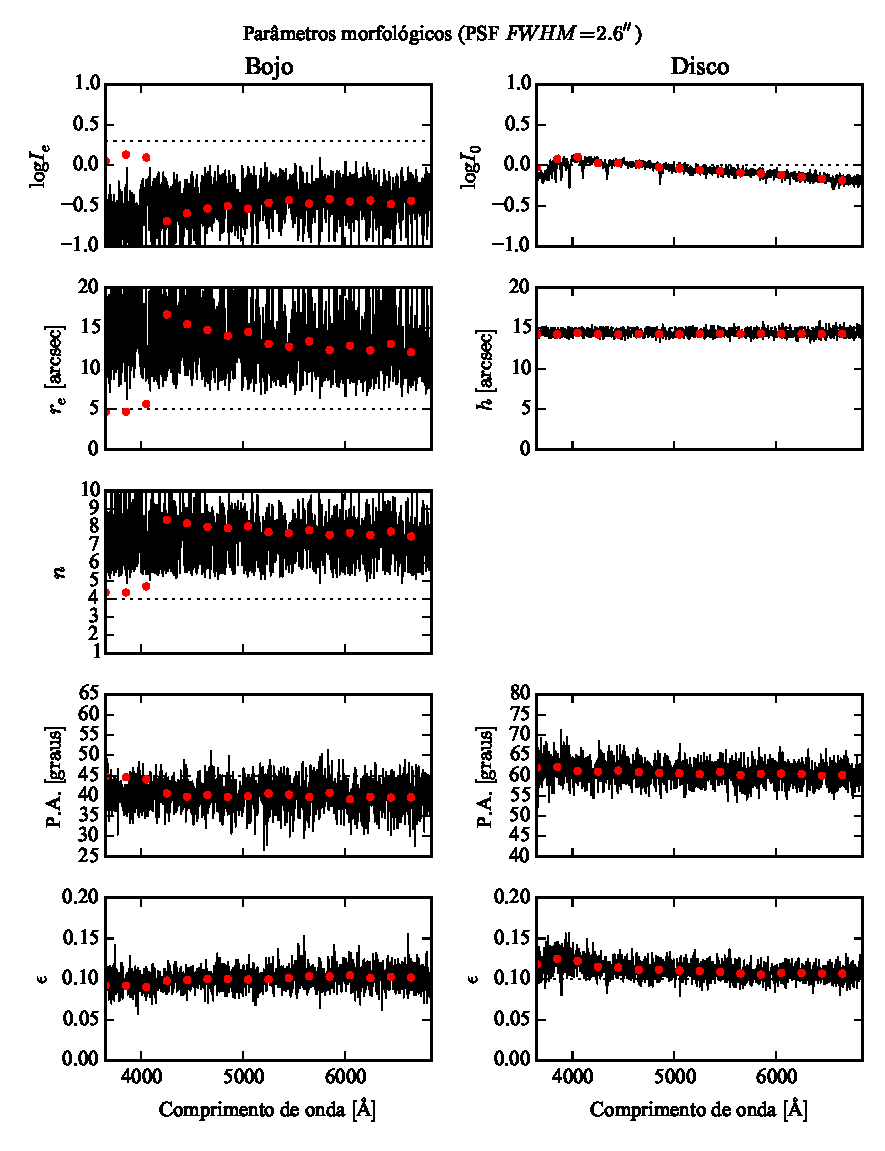
\includegraphics{figuras/simulation_fitparams_psf26}
	\caption[Parâmetos morfológicos (teste com PSF $\mathrm{FWHM} = 2,6\,\arcs$).]
	{Parâmetos morfológicos da galáxia sintética, em função do comprimento de
	onda. Ajuste feito com uma PSF de $\mathrm{FWHM} = 2,6\,\arcs$. Ver
	legenda da Figura \ref{fig:testFitParams}.}
	\label{fig:testFitParams26}
\end{figure}

\begin{figure}
	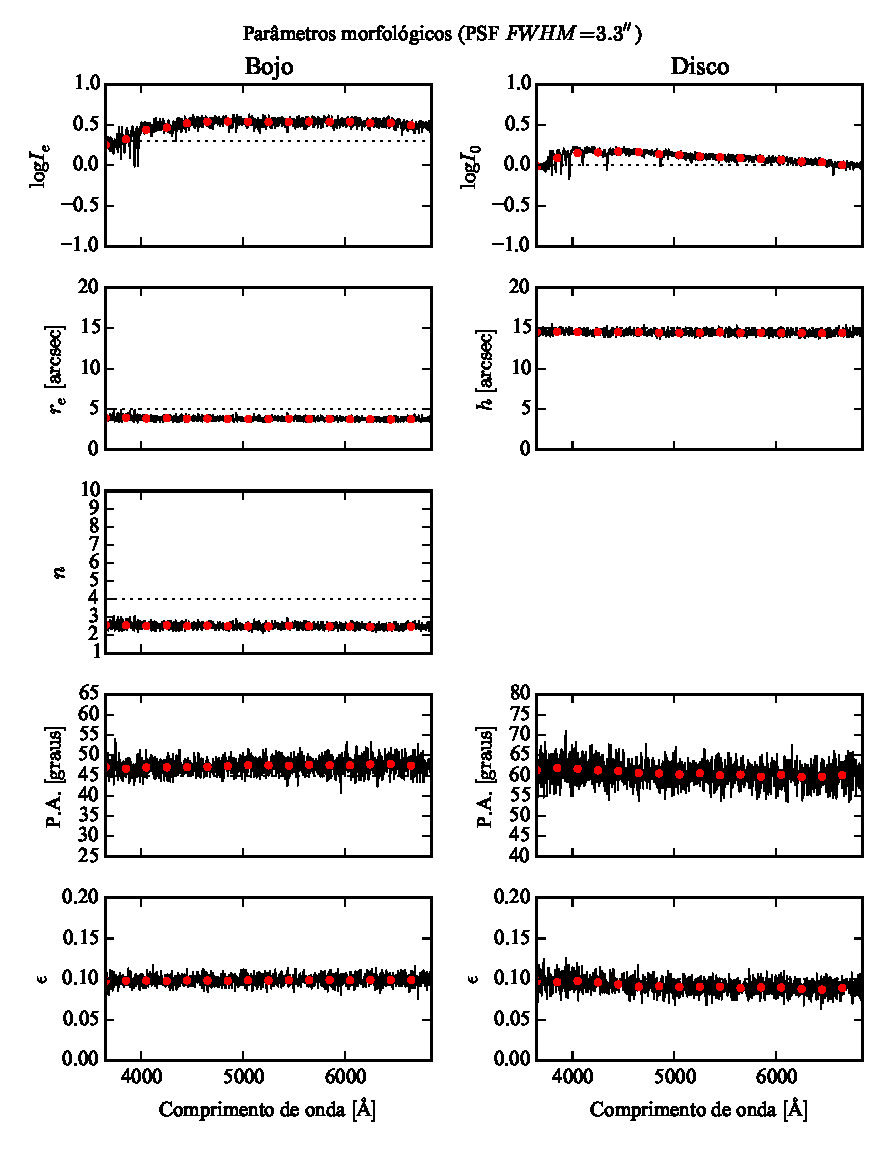
\includegraphics{figuras/simulation_fitparams_psf33}
	\caption[Parâmetos morfológicos (teste com PSF $\mathrm{FWHM} = 3,3\,\arcs$).]
	{Parâmetos morfológicos da galáxia sintética, em função do comprimento de
	onda. Ajuste feito com uma PSF de $\mathrm{FWHM} = 3,3\,\arcs$. Ver
	legenda da Figura \ref{fig:testFitParams}.}
	\label{fig:testFitParams33}
\end{figure}

As Figuras \ref{fig:testFitParams26} e \ref{fig:testFitParams33} mostram os
parâmetros morfológicos obtidos para os dois casos. Pode-se ver que os
parâmetros obtidos para o disco são muito próximos dos parâmetros do teste
anterior. Não é de se estranhar, o disco é muito suave, não tem estruturas na
escala de tamanho da PSF. O bojo, por outro lado, é muito afetado pela má
escolha da PSF. Sobreestimar a FWHM da PSF ($2,6\,\arcs$) faz os valores de
$r_e$ e $n$ aumentarem muito, para cerca de $13\,\arcs$ e $7$, respectivamente.
Também aumenta a dispersão nos dois parâmetros, provavelmente causado por
degenerescência no ajuste. Com a FWHM subestimada ($3,3\,\arcs$), os valores
destes parâmetros diminui, com $r_e \sim 4\,\arcs$ e $n \sim 2,5$. O disco muda
pouco, como no outro caso. Os parâmetros médios das duas decomposições são:

\begin{tabular}{ l  r | l  r }
  \hline
  \multicolumn{4}{c}{Ajuste (PSF $\mathrm{FWHM} = 2,6\,\arcs$)} \\
  \multicolumn{2}{c}{Bojo} & \multicolumn{2}{c}{Disco} \\
  \hline
  $r_e$ & $13,639 \pm 5.217\,\arcs$ & $h$ & $14,398 \pm 0.377\,\arcs$ \\
  $n$ & $7,380 \pm 1,247$ & & \\
  $\mathrm{P.A.}$ & $60,687 \pm 2,624^\circ$ & $\mathrm{P.A.}$ & $40,222
  \pm 3.596^\circ$ \\
  $\epsilon$ & $0,111 \pm 0,011$ & $\epsilon$ & $0,101 \pm 0,012$ \\
  \hline
\end{tabular}

\begin{tabular}{ l  r | l  r }
  \hline
  \multicolumn{4}{c}{Ajuste (PSF $\mathrm{FWHM} = 3,3\,\arcs$)} \\
  \multicolumn{2}{c}{Bojo} & \multicolumn{2}{c}{Disco} \\
  \hline
  $r_e$ & $3,826 \pm 0,206\,\arcs$ & $h$ & $14,466 \pm 0,271\,\arcs$ \\
  $n$ & $2,509 \pm 0,133$ & & \\
  $\mathrm{P.A.}$ & $60,535 \pm 2,563^\circ$ & $\mathrm{P.A.}$ & $47.354 +/-
  1.694^\circ$ \\
  $\epsilon$ & $0,092 \pm 0,008$ & $\epsilon$ & $0,099 \pm 0,005$ \\
  \hline
\end{tabular}

\begin{figure}
	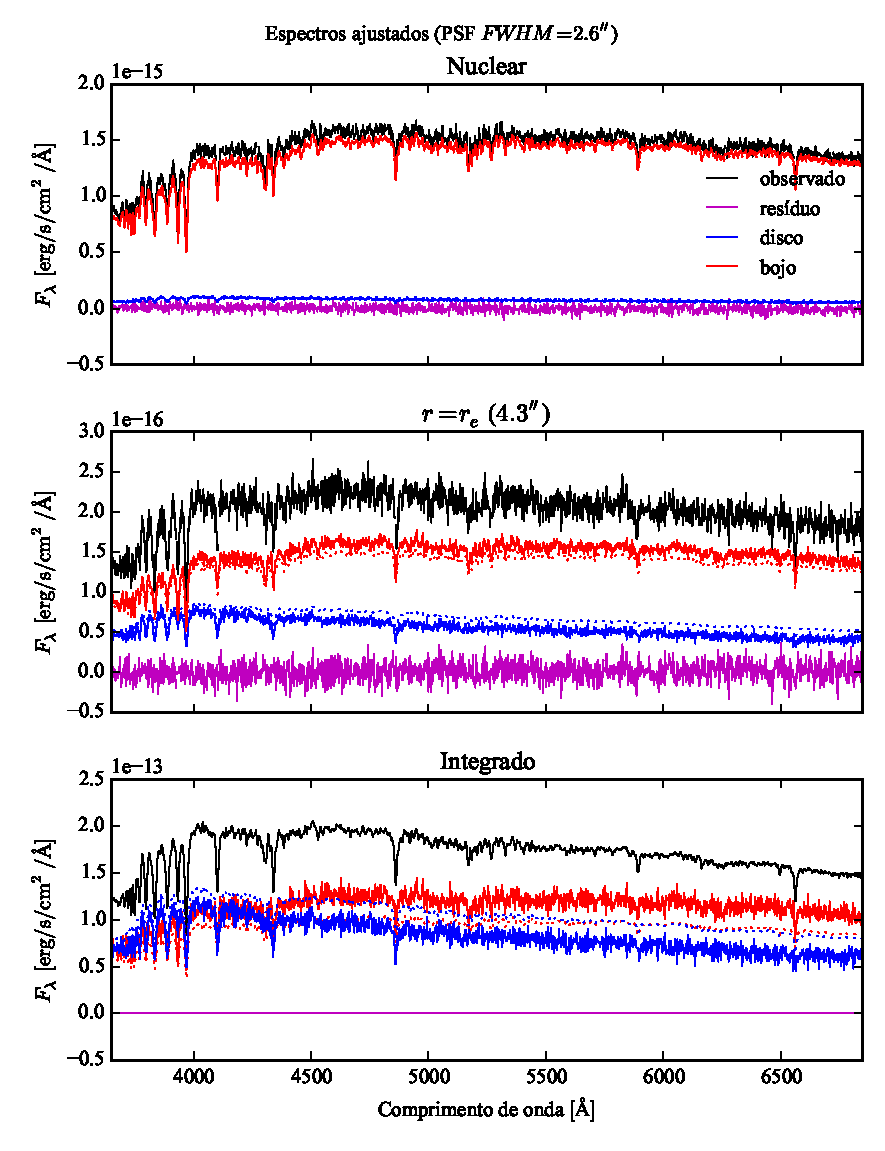
\includegraphics{figuras/simulation_spectra_psf26}
	\caption[Espectros ajustados (teste com PSF $\mathrm{FWHM} = 2,6\,\arcs$).]
	{Espectros ajustados à galáxia sintética. Ajuste feito com uma PSF de
	$\mathrm{FWHM} = 2,6\,\arcs$. Ver legenda da Figura \ref{fig:testFitSpectra}.}
	\label{fig:testFitSpectra26}
\end{figure}

\begin{figure}
	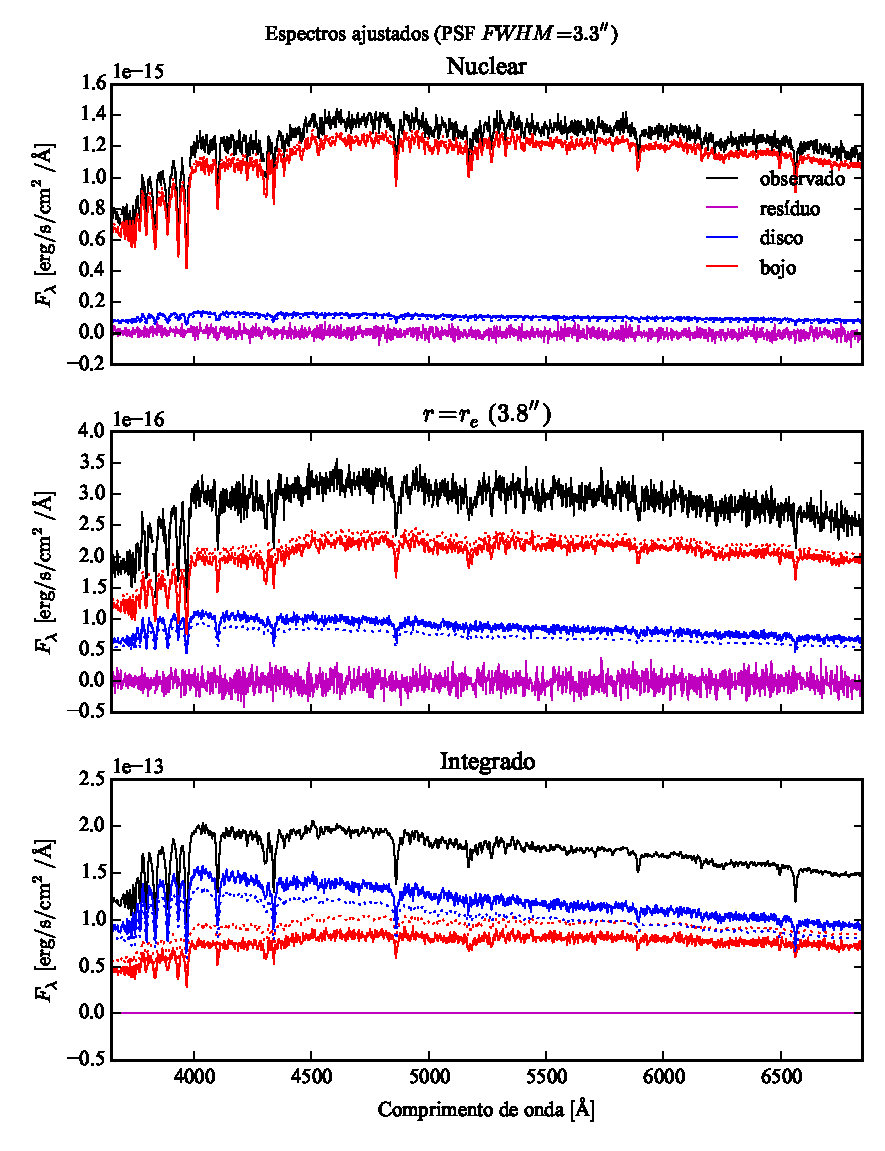
\includegraphics{figuras/simulation_spectra_psf33}
	\caption[Espectros ajustados (teste com PSF $\mathrm{FWHM} = 3,3\,\arcs$).]
	{Espectros ajustados à galáxia sintética. Ajuste feito com uma PSF de
	$\mathrm{FWHM} = 3,3\,\arcs$. Ver legenda da Figura \ref{fig:testFitSpectra}.}
	\label{fig:testFitSpectra33}
\end{figure}

A dispersão nos parâmetros do bojo, no caso sobreestimado, parece um problema em
potecial. Mas, percebe-se que a dispersão nas parâmetros não se reflete tanto
nos espectros, como mostra a Figura \ref{fig:testFitSpectra26}. Os espectros são
parecidos com os originais, com diferenças sistemáticas e um ``ruído'' maior do
que o ajuste com a PSF correta. No caso subestimado, os espectros parecem melhor
ajustados (Figura \ref{fig:testFitSpectra33}), mas também com com diferenças
sistemáticas.

\begin{figure}
	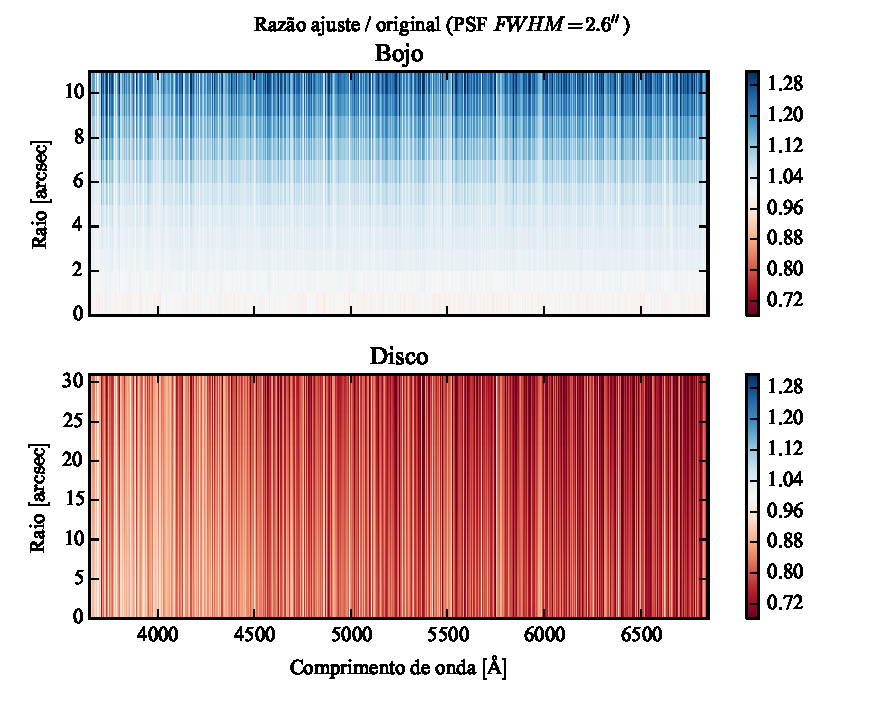
\includegraphics{figuras/simulation_error_psf26}
	\caption[Razão ajuste--original (teste com PSF $\mathrm{FWHM} = 2,6\,\arcs$).]
	{Razão ajuste--original média dos espectros ajustados à galáxia sintética.
	Ajuste feito com uma PSF de $\mathrm{FWHM} = 2,6\,\arcs$. Ver legenda da Figura
	\ref{fig:testFitError}.}
	\label{fig:testFitError26}
\end{figure}

\begin{figure}
	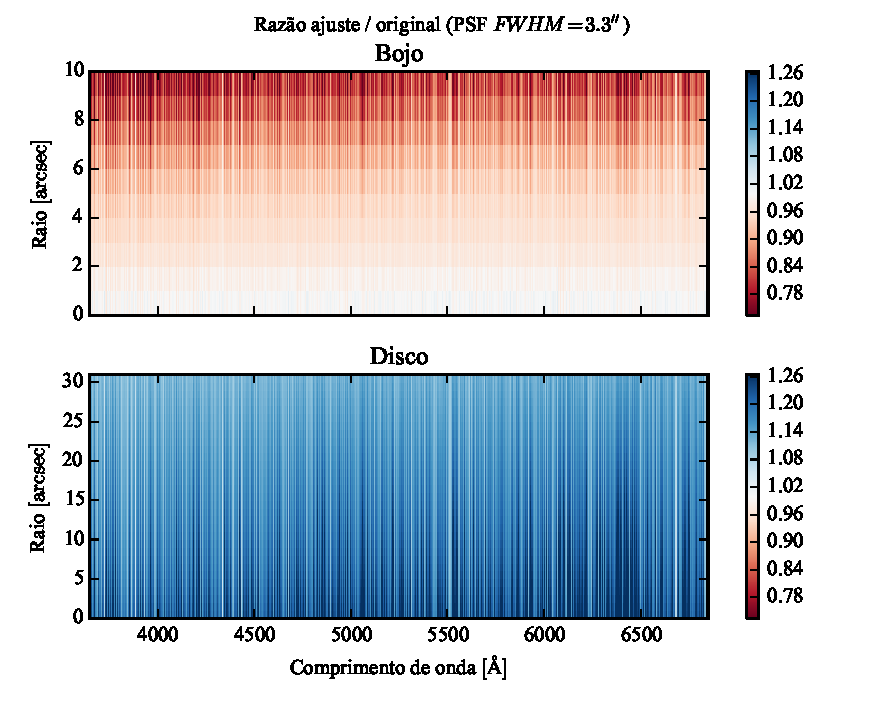
\includegraphics{figuras/simulation_error_psf33}
	\caption[Razão ajuste--original (teste com PSF $\mathrm{FWHM} = 3,3\,\arcs$).]
	{Razão ajuste--original média dos espectros ajustados à galáxia sintética.
	Ajuste feito com uma PSF de $\mathrm{FWHM} = 3,3\,\arcs$. Ver legenda da Figura
	\ref{fig:testFitError}.}
	\label{fig:testFitError33}
\end{figure}

Fazendo a razão ajuste--original (Figura \ref{fig:testFitError26}), percebe-se
que espectro ajustado do bojo torna-se maior do que o original conforme se
afasta do centro, enquanto o disco apresenta um gradiente espectral, ficando
mais azul, quando se sobreestima a FWHM. As ``linhas espectrais artificiais''
neste caso são bem pronunciadas. A razão média para o bojo é de $1,0627 \pm
0,0645$, e para o disco de $0,7721 \pm 0,0823$. Quando se subestima a FWHM
(Figura \ref{fig:testFitError33}), o espectro ajustado do bojo é menor e do que
o original, e diminui com o raio. O Disco não parece ter gradiente radial, e em
ambos os casos, não há um gradiente espectral perceptível, com ``linhas
espectrais artificiais'' menos intensas do que no outro caso. A razão média
neste caso é $0,9355 \pm 0,0532$ para o bojo e $1,1297 \pm 0.0413$ para o disco.

Ao se utilizar, na decomposição morfológica, uma PSF com FWHM maior do que a
real (superestimando), é impossível criar um modelo com um bojo tão concentrado
quanto o observado. O que acontece então é que o algoritmo chega nos modelos
mais próximos, que não representam exatamente a galáxia. O mesmo não ocorre
quando se utiliza uma FWHM menor. Neste caso, basta fazer um bojo menos
concentrado ($r_e$ e/ou $n$ menor). Pelo teste, este caso é mais estável, isto é
possui menos degenerescência.

Assim, pode-se ficar tentado a utilizar a PSF com FWHM menor na decomposição
morfológica espectral das as galáxias do CALIFA, a fim de evitar os caso onde a
PSF dos dados é menor do que $2,9\,\arcs$. Entretanto, deve-se lembrar que o
ajuste é significativamente melhor quando se usa a PSF correta, assim, o melhor
é utilizar a PSF mais frequente da distribuição, de $\mathrm{FWHM} =
2,9\,\arcs$.


%% End of this chapter

  
  % Decomposição e síntese de populações estelares
  %%%%%%%%%%%%%%%%%%%%%%%%%%%%%%%%%%%%%%%%%%%%%%%%%%%%%%%%%%%%%%%%%
% Tese de Doutorado / Dept Fisica, CFM, UFSC                    %
% Andre@UFSC - 2014                                             %
%%%%%%%%%%%%%%%%%%%%%%%%%%%%%%%%%%%%%%%%%%%%%%%%%%%%%%%%%%%%%%%%%

%:::::::::::::::::::::::::::::::::::::::::::::::::::::::::::::::%
%                                                               %
%                          Capítulo 7                           %
%                                                               %
%:::::::::::::::::::::::::::::::::::::::::::::::::::::::::::::::%

%***************************************************************%
%                                                               %
%                        Decomposicao                           %
%                                                               %
%***************************************************************%

\chapter{Decomposição morfológica espectral de galáxias}
\label{sec:Decomp}

%***************************************************************%
%                                                               %
%               Decomposição: decomposicao espectral            %
%                                                               %
%***************************************************************%

\section{O procedimento de decomposição morfológica espectral}

A decomposição morfológica espectral apresentada neste capítulo foi desenhada
para trabalhar com galáxias lenticulares (S0), que podem ser decompostas em um
bojo e um disco. Conforme a Seção \ref{sec:morph:comp:bd}, o perfil de brilho do
bojo é modelado como uma lei de Sérsic, e o perfil do disco como uma lei
exponencial, conforme as equações
\begin{equation*}
I(r) = I_e \exp \left\{- b_n \left[ \left( \frac{a}{r_e} \right)^{1/n}
- 1 \right] \right\},
\end{equation*}
\begin{equation*}
I(r) = I_0 \exp\left(\frac{r}{h}\right).
\end{equation*}

Diferente do método de \citeauthor{Johnston2012}, os perfis do bojo e do disco
são tratados em duas dimensões como elipsoides, cada qual com uma elipticidade
($\epsilon$) e um ângulo de posição (P.A.) independentes. O ângulo de posição é
medido em sentido anti-horário a partir do eixo horizontal positivo. Estes
modelos são ajustados a imagens em cada comprimento de onda, utilizando o
programa IMFIT, conforme descrito na seção a seguir. A decomposição é realizada
sobre os espectros observados. As linhas de emissão são mascaradas, pois estamos
interessados apenas na distribuição de populações estelares.
O ajuste morfológico é feito deixando livres todos os parâmetros das equações
acima ($I_e$, $r_e$, $n$, $I_0$, $h$) e a geometria de cada componente (P.A. e
$\epsilon$), sem fazer hipótese alguma sobre como os parâmetros morfológicos
variam a cada comprimento de onda.

Conforme descrito na Seção \ref{sec:psf:medida}, convolui-se as imagens do
modelo com uma PSF de perfil de Moffat com $\beta=4$ e
$\mathrm{FWHM}=2,9\,\arcs$. Possíveis efeitos causados por uma PSF mal
dimensionada foram vistos na Seção \ref{sec:test:psf}. Esta é uma preocupação
muito relevante no caso do CALIFA, pois em geral os bojos estão mal resolvidos.

% TODO: repensar esta seção
%\subsection{A biblioteca python-imfit}

%\TODO vender o jabá - mini-tutorial do python-imfit?


\subsection{Cinemática}
\label{sec:Decomp:cinematica}

Antes de começar a decomposição, é preciso refletir um pouco sobre a cinemática
das estrelas da galáxia. As estrelas estão distribuídas em bojos e discos, e a
cinemática em cada um dos casos é diferente.
A estrutura plana dos discos é causada por um alto momento angular, com um campo
de velocidades sistêmico projetado na linha de visada. Isto faz com que uma dada
linha espectral tenha um {\em redshift} diferente, dependendo da sua posição no
disco. Já os bojos são normalmente caracterizados por baixa rotação, mas uma
grande dispersão de velocidades, crescendo a medida que se aproxima do centro.
Ou seja, as linhas são mais alargadas nas regiões centrais.

Para que a decomposição morfológica espectral faça sentido, é preciso ter
certeza que, em uma imagem em uma dada janela espectral, se esteja observando os
mesmos processos físicos em todos os {\em spaxel}. Por exemplo, não se pode ter
um {\em spaxel} que contenha fluxo proveniente do fundo de uma linha de
absorção, enquanto outro {\em spaxel} contém fluxo do contínuo adjacente.
Chega-se então num problema cíclico. É preciso saber as características das
componentes morfológicas para que se conheça a cinemática de cada uma delas.
Porém, sem compensar os efeitos da cinemática, não se pode fazer a decomposição
de forma confiável.

O que se faz aqui é obter uma medida aproximada da cinemática, medindo apenas
uma velocidade sistêmica ($v_0$) e uma distribuição de velocidades gaussiana
($v_d$) para cada {\em spaxel}. Isto não é o ideal, pois bojos podem ter alguma
rotação e discos podem ter alguma dispersão de velocidades. A cinemática pode
até ser diferente para cada cada população estelar em uma mesma componente.
Entretanto, isto é uma boa primeira aproximação. A medida de $v_0$ e $v_d$ foi
obtida utilizando o \starlight, que ajusta a cinemática juntamente às populações
estelares.

Corrigir efeitos de $v_0$ é simples, basta aplicar um {\em redshift} (ou {\em
blueshift}) de mesma velocidade, na direção oposta, tal que os espectros fiquem
todos em {\em rest frame}. Já $v_d$ requer um pouco mais de consideração, pois
não é possível ``desalargar'' as linhas espectrais. O que se faz então é tentar
deixar todos os {\em spaxels} com a mesma dispersão de velocidades, degradando a
resolução do espectro. Se a distribuição de velocidades na linha de visada segue
uma distribuição gaussiana, isto é obtido convoluindo (em espaço de velocidades)
o fluxo cada {\em spaxel} com uma gaussiana de largura dada por um $v_{d,\ast}$
adequado, isto é
\begin{equation*}
F_{\lambda,\ast} = \frac{1}{v_{d,\ast}\sqrt{2\pi}}\int_{-\infty}^{+\infty}
F_\lambda \left(\lambda^\prime = \frac{\lambda}{1 + v/c}\right) \exp \left[ -\frac{1}{2}
(v/v_{d,\ast})^2 \right] \mathrm{d}v.
\end{equation*}
Dado que, quando se convolui duas gaussianas, suas dispersões se somam em
quadratura, $v_{d,\ast}$ deve ser tal que o fluxo final tenha a dispersão
alvo $v_{d,\mathrm{alvo}}$. Ou seja,
\begin{equation*}
v_{d,\ast} = \sqrt{v_{d,\mathrm{alvo}} - v^2_d}.
\end{equation*}

\begin{figure}
	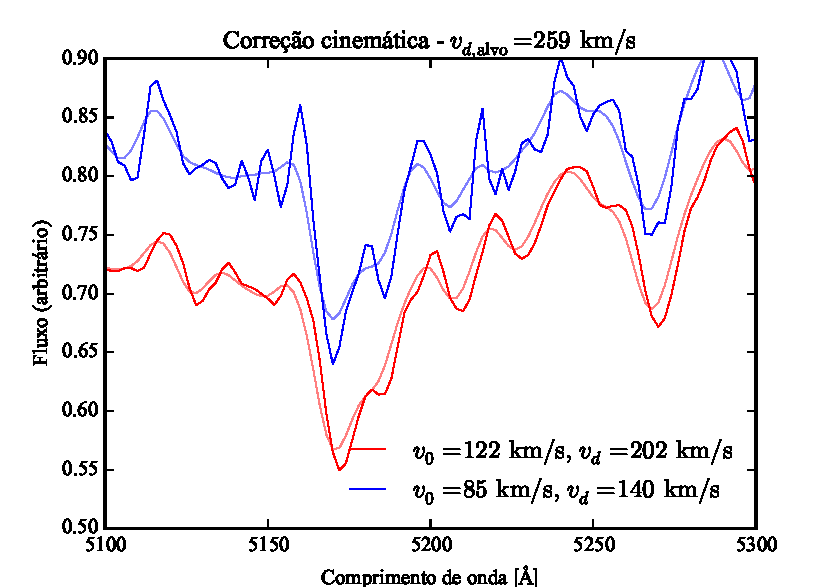
\includegraphics{figuras/cinematica}
	\caption[Correção de efeitos da cinemática]
	{Correção de efeitos da cinemática. Linhas escuras: dois espectros com
	cinemática diferente. Linhas claras: espectros deslocados para {\em rest
	frame}, com as linhas alargadas para uma dispersão de velocidades
	$v_{d,\mathrm{alvo}} = 259\,\mathrm{km}/\mathrm{s}$. O fluxo está em unidades
	arbitrárias para melhor visualização.}
	\label{fig:cinematica}
\end{figure}

Deve-se escolher $v_{d,\mathrm{alvo}}$ de modo que $v_{d,\ast}$ seja sempre um
número real, ou seja, $v_{d,\mathrm{alvo}} > v_d$, para todos os {\em spaxels}.
Na prática, alguns cubos podem ter uns poucos {\em spaxels} com $v_d$ anômalo
(tanto por ajuste ruim pelo \starlight quanto por uma dispersão realmente
grande). Neste caso, a resolução espectral seria degradada enormemente por conta
de um punhado de {\em spaxels}. A solução encontrada foi usar um
$v_{d,\mathrm{alvo}}$ maior do que $95\%$ dos $v_d$, e não fazendo a convolução
nos poucos casos onde $v_d > v_{d,\mathrm{alvo}}$. A Figura \ref{fig:cinematica}
ilustra o efeito da correção de cinemática em {\em spaxels} com cinemática
distinta. Pode-se ver que as linhas espectrais tendem a ficar coerentes após a
correção.


\subsection{Propagação de erros nos espectros}

Em alguns passos da decomposição, são tomadas imagens dos cubos espectrais em
caixas com uma determinada largura em comprimento de onda. Os espectros são
empilhados formando uma imagem, e os erros devem ser propagados de acordo. Os
espectros do CALIFA, na configuração V500, têm uma PSF espectral gaussiana de
$\mathrm{FWHM}=6\,\angstrom$. Porém, a amostragem é feita em caixas de
$2\,\angstrom$. Isto que dizer que fluxos estão correlacionados, logo deveria-se
trabalhar com a matriz de covariância, ao invés de um espectro de erros (ou
incerteza). Entretanto, somente o espectro de erros está disponível nos cubos de
dados do CALIFA (e na maioria dos espectros astronômicos). Note que o mesmo
raciocínio de propagação de erros se aplica à correção de cinemática descrita
anteriormente, com a gaussiana da dispersão de velocidades fazendo o papel de um
peso na soma dos espectros.

Sem a matriz de covariância, há duas alternativas. Se erros nos fluxos estão
correlacionados com dependência na distância espectral de forma a depender
apenas da distância, isto é, uma função $p(\lambda^\prime -
\lambda^{\prime\prime})$, pode-se calcular a correção que a covariância causaria
numa soma ponderada de fluxo. O fluxo médio $F$ ponderado pelos pesos
$w_\lambda$ é dado por
\begin{equation*}
F = \frac{\sum\limits_\lambda w_\lambda F_\lambda}{\sum\limits_\lambda
w_\lambda}.
\end{equation*}
Geralmente se normaliza os erros tal que $\sum\limits_\lambda
w_\lambda = 1$, para simplificar os cálculos. O erro $\sigma_F$ sobre o fluxo
médio $F$ é, levando em conta a correlação,
\begin{equation*}
\sigma_F^2 = \sum\limits_\lambda w_\lambda^2 \sigma_\lambda^2 +
\sum\limits_{\lambda^\prime}
\sum\limits_{\lambda^{\prime\prime}}^{\lambda^{\prime\prime} \neq
\lambda^\prime} p(\lambda^\prime - \lambda^{\prime\prime}) w_{\lambda^\prime}
w_{\lambda^{\prime\prime}} \sigma_{\lambda^\prime}
\sigma_{\lambda^{\prime\prime}}.
\end{equation*}
Para erros gaussianos, $p(\Delta \lambda) \sim \exp\left[-1/2
(\Delta\lambda / c_\mathrm{FWHM})^2\right]$, normalizado. A distância de
covariância é dada por $\mathrm{FWHM} = 2 \sqrt{2 \ln 2}\ c_\mathrm{FWHM}$. Se
os erros não estiverem correlacionados (isto é, se $\mathrm{FWHM} \to 0$),
$p(\Delta \lambda) = 0$, a segunda soma desaparece e o erro é dado pela soma
ponderada usual.

A segunda alternativa é estimar o erro a partir dos dados. Isto só funciona
quando a soma é feita sobre uma caixa espectral com um grande número de medidas.
Neste caso, o erro é dado pela covariância amostral,
\begin{equation*}
\sigma_F^2 = \dfrac{\sum\limits_\lambda w_\lambda}{\left(\sum\limits_\lambda
w_\lambda\right)^2 - \sum\limits_\lambda w_\lambda^2} \sum\limits_\lambda
w_\lambda \left(F_\lambda - F\right)^2.
\end{equation*}

A primeira alternativa é utilizada na convolução de velocidades, pois em geral
cada elemento do espectro convoluído contém fluxo proveniente de poucas medidas.
A segunda é utilizada ao se empilhar espectros em caixas de comprimento de onda
de largura maior que $100\,\angstrom$, para uma estimativa mais realista do
erro. Quando se calcula a imagem média numa caixa, neste trabalho, o peso na
soma ponderada dos fluxos é dado por $w_\lambda = \sigma_\lambda^{-2}$, ou seja,
o inverso dos erros provenientes dos cubos de dados, ao quadrado.


\subsection{Modelos iniciais e ajuste a cada comprimento de onda}
\label{sec:Decomp:initmodel}

A decomposição morfológica espectral requer, nesta implementação, um número de
ajustes morfológicos igual ao número de amostras de comprimento de onda. Para
cubos com a configuração V500, são 1600 amostras de largura $2\,\angstrom$. Isto
requer que se utilize um algoritmo rápido para fazer o ajuste. Para o programa
IMFIT \citep{Erwin2015}, este algoritmo é o L-M (ver a descrição dos algoritmos
na Seção \ref{sec:morph:comp:ajuste}). Para fazer um ajuste utilizando L-M, é
preciso ter um bom chute inicial, visto que este algoritmo é muito propenso a
cair em mínimos locais. Este chute inicial é determinado utilizando os outros
algoritmos mais lentos, N-M e DE.

Como primeira aproximação, toma-se uma caixa de $100\,\angstrom$ ao redor de
$5635\,\angstrom$ (comprimento de onda de normalização) e calcula-se as imagens
de fluxo e erro conforme visto na seção anterior. Esta imagem é utilizada para
calcular o chute inicial nos parâmetros morfológicos, utilizando as seguintes
heurísticas:
\begin{enumerate}
  \item Encontrar o raio que contém metade da luz ($\mathrm{HLR}$), que é, em
  primeira aproximação, o local mais provável para que a componente dominante
  deixe de ser o bojo e passe a ser o disco \cite{GonzalezDelgado2015};
  \item Mascarar a região central ($r < \mathrm{HLR}$);
  \item Criar um modelo de disco de $h=1,5 \mathrm{HLR}$ utilizando DE;
  \item Ajustar o disco á imagem mascarada;
  \item Criar um modelo de bojo com $n = 4$ e $r_e = 0,5 \mathrm{HLR}$;
  \item Ajustar os modelo de bojo e disco (já ajustado anteriormente) à imagem
  completa utilizando DE;
  \item Refinar o ajuste utilizando N-M, depois L-M.
\end{enumerate}

\begin{figure}
	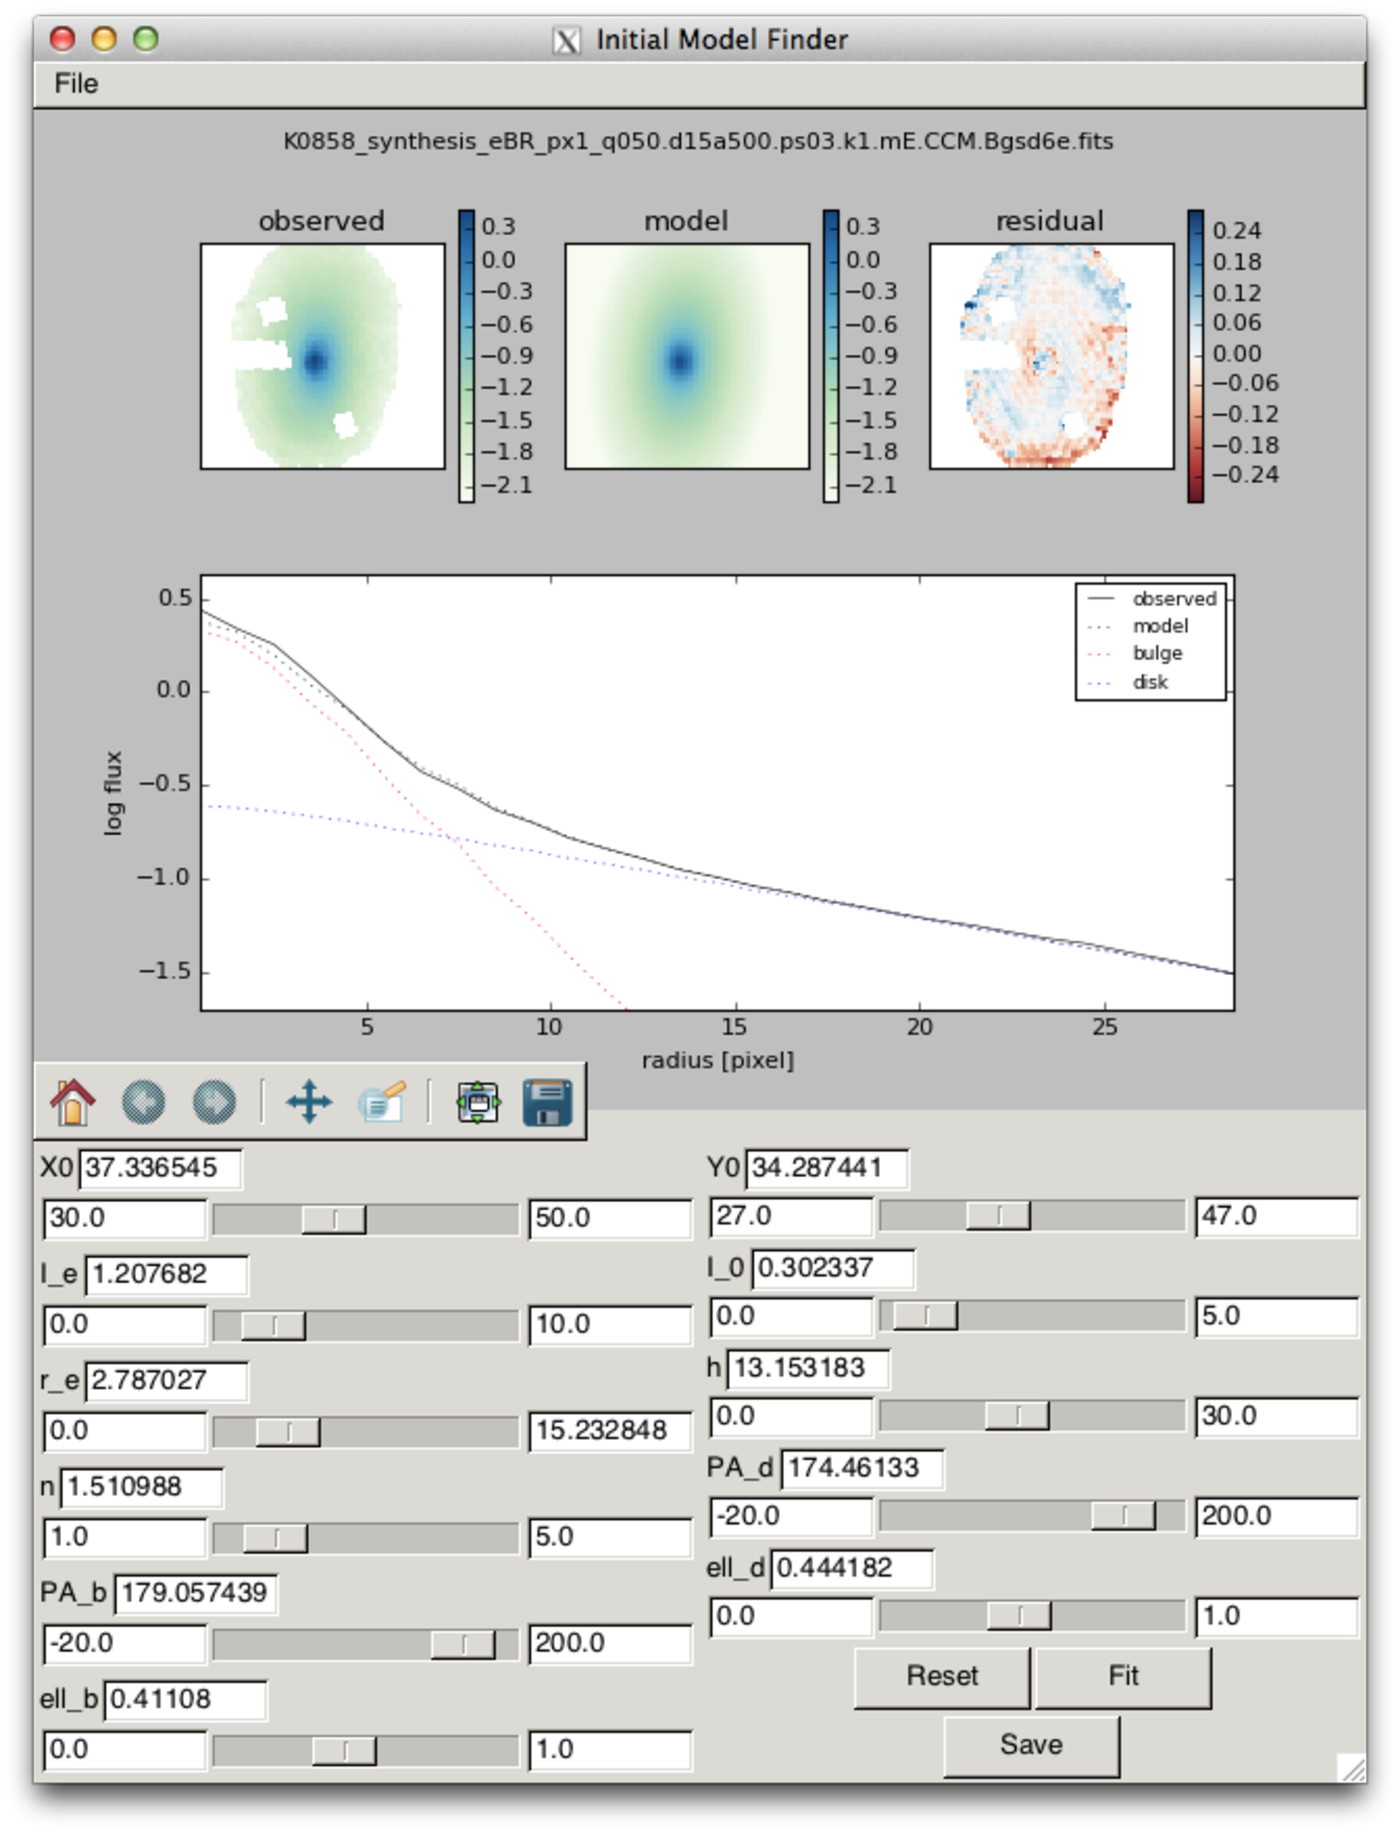
\includegraphics[width=1.0\columnwidth]{figuras/model_finder}
	\caption[Programa gráfico para encontrar o modelo inicial]
	{Programa gráfico para encontrar o modelo inicial de forma interativa.}
	\label{fig:modelFinder}
\end{figure}

Este procedimento é computacionalmente intensivo, e o conjunto de heurísticas
foi determinado de forma empírica. Ainda assim, ele falha em muitos casos,
geralmente precisando ser modificado caso a caso. O tempo típico, em um
computador atual, de ajuste do modelo inicial é de 10 minutos. É possível fazer
este ajuste de forma interativa, utilizando uma ferramenta gráfica, numa fração
deste tempo. Com este objetivo foi desenvolvido o programa mostrado na Figura
\ref{fig:modelFinder}. Com ele pode-se escolher modelos iniciais, limites, e
fazer um ajuste de teste, tudo em tempo real. Como a amostra é pequena, um
programa interativo ainda é uma abordagem viável.

Como visto na Seção \ref{sec:morph:comp:depLambda}, os parâmetros morfológicos
podem depender do comprimento de onda. Logo, um único modelo inicial pode não
ser suficiente para escapar dos mínimos locais. Assim, utiliza-se imagens em
caixas de $100\,\angstrom$, e espaçadas em intervalos também de
$100\,\angstrom$, para fazer ajustes utilizando o algoritmo N-M. Obtém-se desta
forma modelos iniciais para cada comprimento de onda. Os parâmetros destes
modelos são, de forma independente, ajustados a polinômios em função de
$\lambda$. Em nenhum caso (da amostra final deste trabalho) houve necessidade de
ajuste de um polinômio de ordem maior que 1, isto é uma reta.

O ajuste morfológico final se dá utilizando os chutes iniciais dados pelos
polinômios dos parâmetros. As imagens são tomadas $\lambda$-a-$\lambda$, sem
combinar imagens. O ajuste é feito utilizando L-M. Caso não haja convergência do
algoritmo, ou o melhor ajuste fique preso em algum limite dos parâmetros, o
ajuste é marcado como falho.

Ao final do ajuste morfológico, cria-se uma imagem para o bojo e para o disco em
cada comprimento de onda. Os cubos de dados espectrais são montados apenas
armazenando estas imagens em ordem de comprimento de onda. Os cubos de dados
espectrais das componentes morfológicos estão prontos para serem analisados como
espectros.


%***************************************************************%
%                                                               %
%                      Seleção da amostra                       %
%                                                               %
%***************************************************************%

\section{Seleção da amostra de galáxias}

A amostra para candidatos à decomposição morfológica espectral foi selecionada a
partir de 331 galáxias observadas com a configuração V500, as quais passaram
pelo QBICK e tiveram os espectros passados pelo \starlight, sem segmentação em
zonas de Voronoi (ver Seções \ref{sec:ifs:qbick} e \ref{sec:ifs:starlight}).
Isto é necessário para que se tenha medidas da cinemática da galáxia, utilizadas
para preparar os dados antes da decomposição.

O passo seguinte foi selecionar as galáxias conforme seu tipo morfológico. A
classificação morfológica das galáxias da amostra mãe do CALIFA foi feita
visualmente por 5 voluntários, utilizando imagens do SDSS nas bandas $r$ e $i$
\citep{Walcher2014}. Os critérios foram:

\begin{itemize}
  \item Elíptica (E), com subclasse 0--7.
  \item Espiral (S), com subclasses 0, 0a, a, ab, b, bc ,c ,cd, d, m;
  \item Irregular (I);
  \item Em qualquer classe, barra (B), sem barra (A), ou indefinida (AB);
  \item Características de {\em merger} (sim ou não).
\end{itemize}

Os três primeiros itens formam uma sequência numérica segundo a classificação de
Hubble, de 0 a 18. As 5 classificações independentes foram combinadas,
calculando a média (descartando valores atípicos, distante mais de 4 classes da
média). Os valores máximos e mínimos, para dar uma ideia da incerteza, são
calculados utilizando todas as 5 classificações. Foi feita uma filtragem na
lista de galáxias observadas, baseada na tabela de classificação morfológica.
Dada a natureza subjetiva da classificação visual, optou-se por utilizar as
classificações máxima e mínima, de tal forma que seja possível que galáxia em
questão seja da classe S0. Isto é, se a galáxia for classificada como elíptica
($<\mathrm{S0}$), mas a classificação máxima for, por exemplo, Sa
($>\mathrm{S0}$), a galáxia entra na amostra. O inverso também vale, uma galáxia
Sa tiver uma classificação mínima E7, também entra na amostra.
As galáxias também têm que ser sem barra (A), e sem características de {\em
merger}.

Adicionalmente, as galáxias precisam ter uma elipticidade máxima $\epsilon<0,5$,
medida nas imagens do SDSS na banda $r$. Isto é necessário para evitar problemas
na decomposição morfológica, pois o modelo bojo--disco não funciona bem em
sistemas muito inclinados. A amostra inicial é listada no Tabela
\ref{tab:DecompSample} (Anexo \ref{apendice:amostra}).

O programa interativo de ajuste foi utilizado nas 43 galáxias da amostra.
O ajuste não pode ser feito em 19 delas, pois apresentaram características que
não permitem fazer a decomposição morfológica em bojo e disco, como faixas de
poeira ou disco muito fraco. Outras 15 apresentam problemas no ajuste, como
mínimos locais intermitentes ou ausência de alguma componente. A coluna de
observações na Tabela \ref{tab:DecompSample} informa os problemas encontrados em
cada caso. O sumário dos descartes é o seguinte:

\begin{itemize}
  \item Ajuste ruim: 15
  \item Faixa de poeira: 9
  \item Disco fraco: 5
  \item Inclinada: 2
  \item Braço espiral: 1
  \item Irregular: 1
  \item Poucos {\em spaxels}: 1
\end{itemize}

\begin{table}
\begin{tabular}{ l l r r r r l }
\hline
ID & Nome & Classe & Classe (mín.) & Classe (máx.) & $\epsilon$ \\
\hline
K0018 & NGC 0155  &  1 (E1)  & 0 (E0) &  8 (S0)  & $0,22$ \\
K0127 & NGC 1349  &  6 (E6)  & 0 (E0) & 10 (Sa)  & $0,11$ \\
K0592 & NGC 4874  &  0 (E0)  & 0 (E0) &  8 (S0)  & $0,12$ \\
K0602 & NGC 4956  &  1 (E1)  & 0 (E0) &  8 (S0)  & $0,14$ \\
K0832 & NGC 6146  &  5 (E5)  & 3 (E3) &  8 (S0)  & $0,23$ \\
K0846 & UGC 10695 &  5 (E5)  & 2 (E2) &  8 (S0)  & $0,33$ \\
K0851 & NGC 6338  &  5 (E5)  & 1 (E1) &  8 (S0)  & $0,34$ \\
K0858 & UGC 10905 &  9 (S0a) & 7 (E7) & 11 (Sab) & $0,47$ \\
K0912 & NGC 7623  &  8 (S0)  & 8 (S0) &  8 (S0)  & $0,29$ \\
\hline
\end{tabular}
\caption[Amostra final para decomposição morfológica espectral]
{Amostra final para decomposição morfológica espectral.}
\label{tab:DecompSampleFinal}
\end{table}

A identificação dos ajustes ditos ruins foi feita através de inspeção visual,
com um grau considerável de subjetividade. Os critérios incluem, por exemplo, a
presença de mínimos locais intermitentes e degenerados (parâmetros saltando
entre dois patamares com mudança imperceptível no aspecto dos perfis e no
$\chi^2$). Esta seleção foi feita de forma fortemente conservadora. A amostra
final deste trabalho (listada na Tabela \ref{tab:DecompSampleFinal}) consiste em
9 galáxias que tiveram uma decomposição boa segundo estes critérios.


%***************************************************************%
%                                                               %
%                  Decomposição da amostra final                %
%                                                               %
%***************************************************************%
\section{Aplicação da decomposição na amostra final}
\label{sec:Decomp:decomp}

A decomposição morfológica espectral foi realizada nas 9 galáxias da amostra
final. Figuras mostrando o resultado da decomposição de todas as galáxias podem
ser vistas no Apêndice \ref{apendice:Decomp}. Nesta seção é discutido o
resultado apenas para a galáxia em que se obteve a melhor decomposição, K0858
(UGC 10905). Recomenda-se comparar as figuras das outras galáxias com o que está
exposto a seguir.

\begin{figure}
	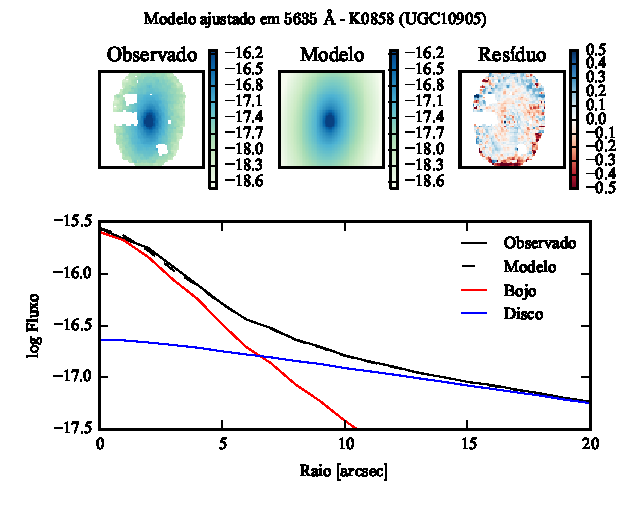
\includegraphics[page=1]{figuras-decomp/K0858_sample006a}
	\caption[Ajuste morfológico em $5635\,\angstrom$ para K0858 (UGC 10905)]
	{Acima: imagens observada, modelada e resíduo, do fluxo em $5635\,\angstrom$
	para K0858 (UGC 10905). Abaixo: perfis radiais, obtidos pela média do fluxo em
	anéis elípticos nas imagens. O fluxo observado é representado pela linha preta
	sólida. O melhor ajuste é representado pela linha preta tracejada. O bojo e o
	disco que compõe o modelo são mostrados em vermelho e azul, respectivamente.}
	\label{fig:decompRadprof}
\end{figure}

A Figura \ref{fig:decompRadprof} permite uma visualização bidimensional, nos
painéis superiores, do fluxo observado, modelo e resíduo em $5635\,\angstrom$.
No resíduo se observa efeitos de borda próximo às regiões externas mascaradas,
além de artefatos seguindo um padrão quase regular\footnote{O padrão hexagonal
que aparece nas imagens (sobretudo nas de resíduo) está relacionado com a forma
como os cubos são reconstruídos.}. Pode-se observar também uma estrutura que
parece ser um braço espiral, em excesso (azul) no resíduo. Isto não é surpresa,
dado que esta galáxia é classificada como S0a. Outra forma de visualizar a
qualidade do ajuste é através do perfil de brilho radial, no painel inferior. O
perfil é calculado utilizando anéis elípticos, com a elipticidade calculada a
partir da imagem observada.

\begin{figure}
	\includegraphics[page=2]{figuras-decomp/K0858_sample006a}
	\caption[Parâmetros morfológicos em função do comprimento de onda para K0858
	(UGC 10905)]
	{Parâmetros morfológicos em função do comprimento de onda para
	K0858 (UGC 10905). Regiões em rosa representam comprimentos de onda onde a
	decomposição falhou. Regiões em cinza foram mascaradas antes de iniciar a
	decomposição. Pontos azuis indicam o primeiro passo da decomposição, em caixas
	de $100\,\angstrom$.}
	\label{fig:decompParams}
\end{figure}

A dependência em $\lambda$ dos parâmetros morfológicos obtidos para K0858 é
mostrada na Figura \ref{fig:decompParams}. As linhas pretas representam a
decomposição final, feita $\lambda$-a-$\lambda$, e os pontos azuis a
decomposição feita no primeiro passo da decomposição, em caixas de
$100\,\angstrom$. Regiões espectrais mascaradas antes de iniciar a decomposição
(onde pode haver emissão de gás) estão marcadas em cinza. Marcadas em rosa estão
regiões espectrais onde a decomposição falhou.

A primeira coisa que chama a atenção na Figura \ref{fig:decompParams} é a
diferença entre as parâmetros morfológicos obtidos em caixas de $100\,\angstrom$
e os obtidos em a cada comprimento de onda. Isto pode ser devido à correção da
cinemática (Seção \ref{sec:Decomp:cinematica}), que praticamente não tem efeito
numa imagem de banda espectral larga. Pode também estar relacionado ao
sinal--ruído das imagens, que aumenta quando se soma imagens. De qualquer forma,
se está interessado no espectro, sendo assim, leva-se em conta apenas a
decomposição final.

Pode-se observar um gradiente espectral no comprimento de escala do disco ($h$).
Já o raio efetivo do bojo ($r_e$) e o índice de Sérsic ($n$), não apresentam um
gradiente apreciável. Todos os parâmetros parecem ter um salto em
$4000\,\angstrom$. Entretanto, o ajuste falha em comprimentos de onda menores,
ficando difícil determinar se isto é um resultado espúrio. Na verdade, qualquer
tentativa de interpretação, observando apenas a dependência dos parâmetros
morfológicos com o comprimento de onda, deve ser feita com cuidado. É esperado
que os parâmetros variem com o comprimento de onda, quando são medidos em bandas
espectrais largas e distantes, como mencionado na Seção
\ref{sec:morph:comp:depLambda}. Entretanto, estas são evidências empíricas, sem
um modelo que as suportem. Tirar conclusões da variação $\lambda$-a-$\lambda$
dos parâmetros pode ser precipitado.

\begin{figure}
	\includegraphics[page=4]{figuras-decomp/K0858_sample006a}
	\caption[Espectro das componentes morfológicas de K0858 (UGC 10905). Acima,
	espectros] {Espectro das componentes morfológicas de K0858 (UGC 10905),
	observado (preto), bojo (vermelho), disco (azul) e resíduo (magenta). Acima:
	Espectro do {\em spaxel} nuclear da galáxia. Meio: Espectro em um {\em spaxel}
	a uma distância de $r_e$ do núcleo. Abaixo: Espectro integrado espacialmente.}
	\label{fig:decompSpectra}
\end{figure}

Os espectros de galáxias, por outro lado, são melhor compreendidos. Mesmo as
menores características dos espectros, como linhas fracas de absorção, podem ser
razoavelmente bem explicadas com modelos de populações estelares. Então, se um
espectro de bojo ou disco tiver o aspecto de um espectro de galáxia, pode-se
começar a levar o resultado da decomposição a sério. A Figura
\ref{fig:decompSpectra} mostra os espectros dos modelos (bojo em vermelho e
disco em azul), no {\em spaxel} nuclear, a $r_e$ de distância do núcleo, e o
espectro integrado dos modelos. O espectro observado é mostrado em preto, e o
resíduo em magenta.

Com uma análise visual, os espectros parecem galáticos. Nos piores casos os
bojos parecem ter um ajuste pior do que os discos, e costumam ter dimensões
comparáveis à largura da PSF. A má resolução dos bojos pode comprometer a
decomposição, nestes casos. Pode-se observar que o resíduo geralmente apresenta
um gradiente nos {\em spaxels}, e praticamente desaparece no espectro integrado.
Este gradiente no resíduo indica que os modelos somados são mais vermelhos do
que o espectro observado. Isto certamente irá afetar o resultado da síntese de
populações estelares, analisada na seção a seguir. Os espectros integrados dos
modelos, se tiverem tal gradiente de cor, devem ter uma forma tal que se
cancelam no resíduo.

%***************************************************************%
%                                                               %
%                        Síntese espectral                      %
%                                                               %
%***************************************************************%
\section{Síntese espectral de populações estelares}
\label{sec:Decomp:sintese}

A síntese espectral de populações estelares, utilizando \starlight foi aplicada
às componentes morfológicas e ao espectro original de todas as galáxias da
amostra final. A base utilizada foi a de Granada--MILES. Dentre as galáxias da
amostra, apenas duas tiveram um ajuste bom com o \starlight: K0592 e K0858. Os
espectros ajustados e as propriedades obtidas para toda a amostra estão no
Apêndice \ref{apendice:Decomp}. A seguir uma discussão sobre o resultado para
K0858.

\begin{figure}
	\includegraphics[page=15,width=\textwidth]{figuras/sample006a_synthesis}
	\caption[Espectros ajustados com \starlight das componentes morfológicas de
	K0858 (UGC 10905)]
	{Acima: Espectros integrados das componentes morfológicas de
	K0858 (UGC 10905), ajustados com \starlight. Em preto, espectro observado. Em
	vermelho, e azul, as componentes bojo e disco. Em linhas de cor clara, o
	espectro ajustado pelo \starlight. Abaixo: Resíduo dos espectros (observado
	menos sintético, divididos pelo observado).}
	\label{fig:decompSinteseSpec}
\end{figure}

A Figura \ref{fig:decompSinteseSpec} mostra ajustes do \starlight para os
espectros integrados observado, do bojo e do disco. As linhas mais claras
mostram o melhor ajuste. No painel inferior, tem-se o resíduo do ajuste em
relação ao espectro de entrada. O ajuste é bom em linhas gerais, embora seja
possível ver alguns pontos onde o resíduo do bojo e do disco estejam
anti-correlacionados, devido à degenerescência do modelo.


\begin{figure}
	\includegraphics[page=16]{figuras/sample006a_synthesis}
	\caption[Propriedades físicas das componentes morfológicas de K0858 (UGC 10905)]
	{Perfil radial de propriedades físicas das componentes morfológicas de
	K0858 (UGC 10905), obtidos através do \starlight. As linhas contínuas
	representam as propriedades obtidas utilizando espectros espacialmente
	resolvidos. As linhas tracejadas representam as propriedades obtidas utilizando
	os espectros integrados. Em preto, espectro observado. Em vermelho, e azul, as
	componentes bojo e disco. Acima, à esquerda: idade estelar média ponderada pela
	luminosidade. Acima, à direita: atenuação por poeira, na banda $V$. Abaixo, à
	esquerda: metalicidade estelar média, ponderada pela massa. Abaixo, à direita:
	densidade superficial de massa estelar. As frações de massa e luminosidade
	entre as componentes e a total (obtida do espectro observado) são indicadas no
	painel inferior, à direita.}
	\label{fig:decompSinteseRadprof}
\end{figure}

As propriedades físicas derivadas da síntese de populações estelares é mostrada
na Figura \ref{fig:decompSinteseRadprof}. Ali, pode-se ver um perfil radial das
propriedades, ajustados nos espectros de cada {\em spaxel}, ou seja,
espacialmente resolvidos, em linhas sólidas. As propriedades derivadas do
espectro integrado são mostradas como linhas tracejadas. Pode-se notar que a
atenuação por poeira $A_V$ (painel superior direito), tanto no bojo quanto no
disco, é muito diferente da atenuação para os espectros observados, quando se
utiliza os espectros espacialmente resolvidos. O mesmo se observa para a idade
estelar média ponderada pela luminosidade (painel superior esquerdo). Estes dois
fatos provavelmente têm relação com o gradiente de cor aparente no resíduo da
decomposição morfológica espectral. A metalicidade estelar média ponderada pela
massa (painel inferior esquerdo), quando espacialmente resolvida, é muito
diferente da calculada no espectro integrado, para todos os casos. A densidade
superficial de massa estelar é mostrada no painel inferior direito. A massa e a
luminosidade das componentes morfológicas, em relação à massa da galáxia
original, são mostrados no mesmo painel. Note que, devido à quantidade de
poeira, a densidade de massa superficial espacialmente resolvida das componentes
morfológicas é maior do que a calculada com o espectro observado.

\begin{figure}
	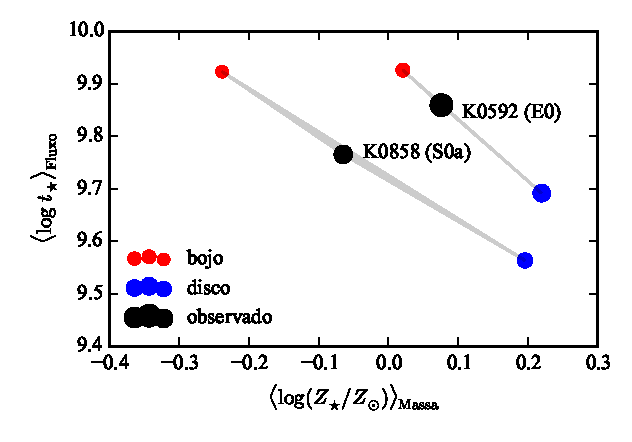
\includegraphics{figuras/sample006a_synthesis_all2}
	\caption[Idade e metalicidade médios das componentes morfológicas]
	{Idade estelar média ponderada pela luminosidade contra metalicidade estelar
	média ponderada pela massa, para as componentes duas morfológicas de
	duas galáxias do CALIFA: K0592 (NGC 4874, E0) e K0858 (UGC10905, S0a). Idades
	e metalicidades foram obtidas pelo \starlight. Pontos em preto são referentes
	ao espectro observado, total da galáxia. Pontos emem vermelho são referentes
	ao bojo, e em azul, ao disco. A área dos círculos indica a massa estelar.}
	\label{fig:decompSintese}
\end{figure}

Estes problemas com a idade estelar e a atenuação por poeira, nos espectros
espacialmente resolvidos, aparece também nas outras galáxias da amostra, mesmo
na outra galáxia com um bom ajuste de populações estelares, a K0592. As
propriedades obtidas com os espectros integrados, por outro lado, parecem melhor
comportadas. A Figura \ref{fig:decompSintese} mostra um gráfico da idade contra
metalicidade estelar, para as componentes morfológicas (bojo em vermelho e disco
em azul) e para o espectro observado (em preto) de K0592 e K0858. A massa da
galáxia (ou da componente morfológica) é representada pela área do círculo.
As duas galáxias, neste gráfico, têm um comportamento similar.
Ambas têm um bojo mais velho e de metalicidade mais baixa, e um disco mais jovem
e de metalicidade mais alta, com relação idade e metalicidade do espectro
observado. Também é interessante notar que os pontos para uma mesma galáxia
estão alinhados. Isto pode acontecer devido à degenerescência entre idade e
metalicidade, comumente vista em sínteses de população estelar.

\begin{figure}
	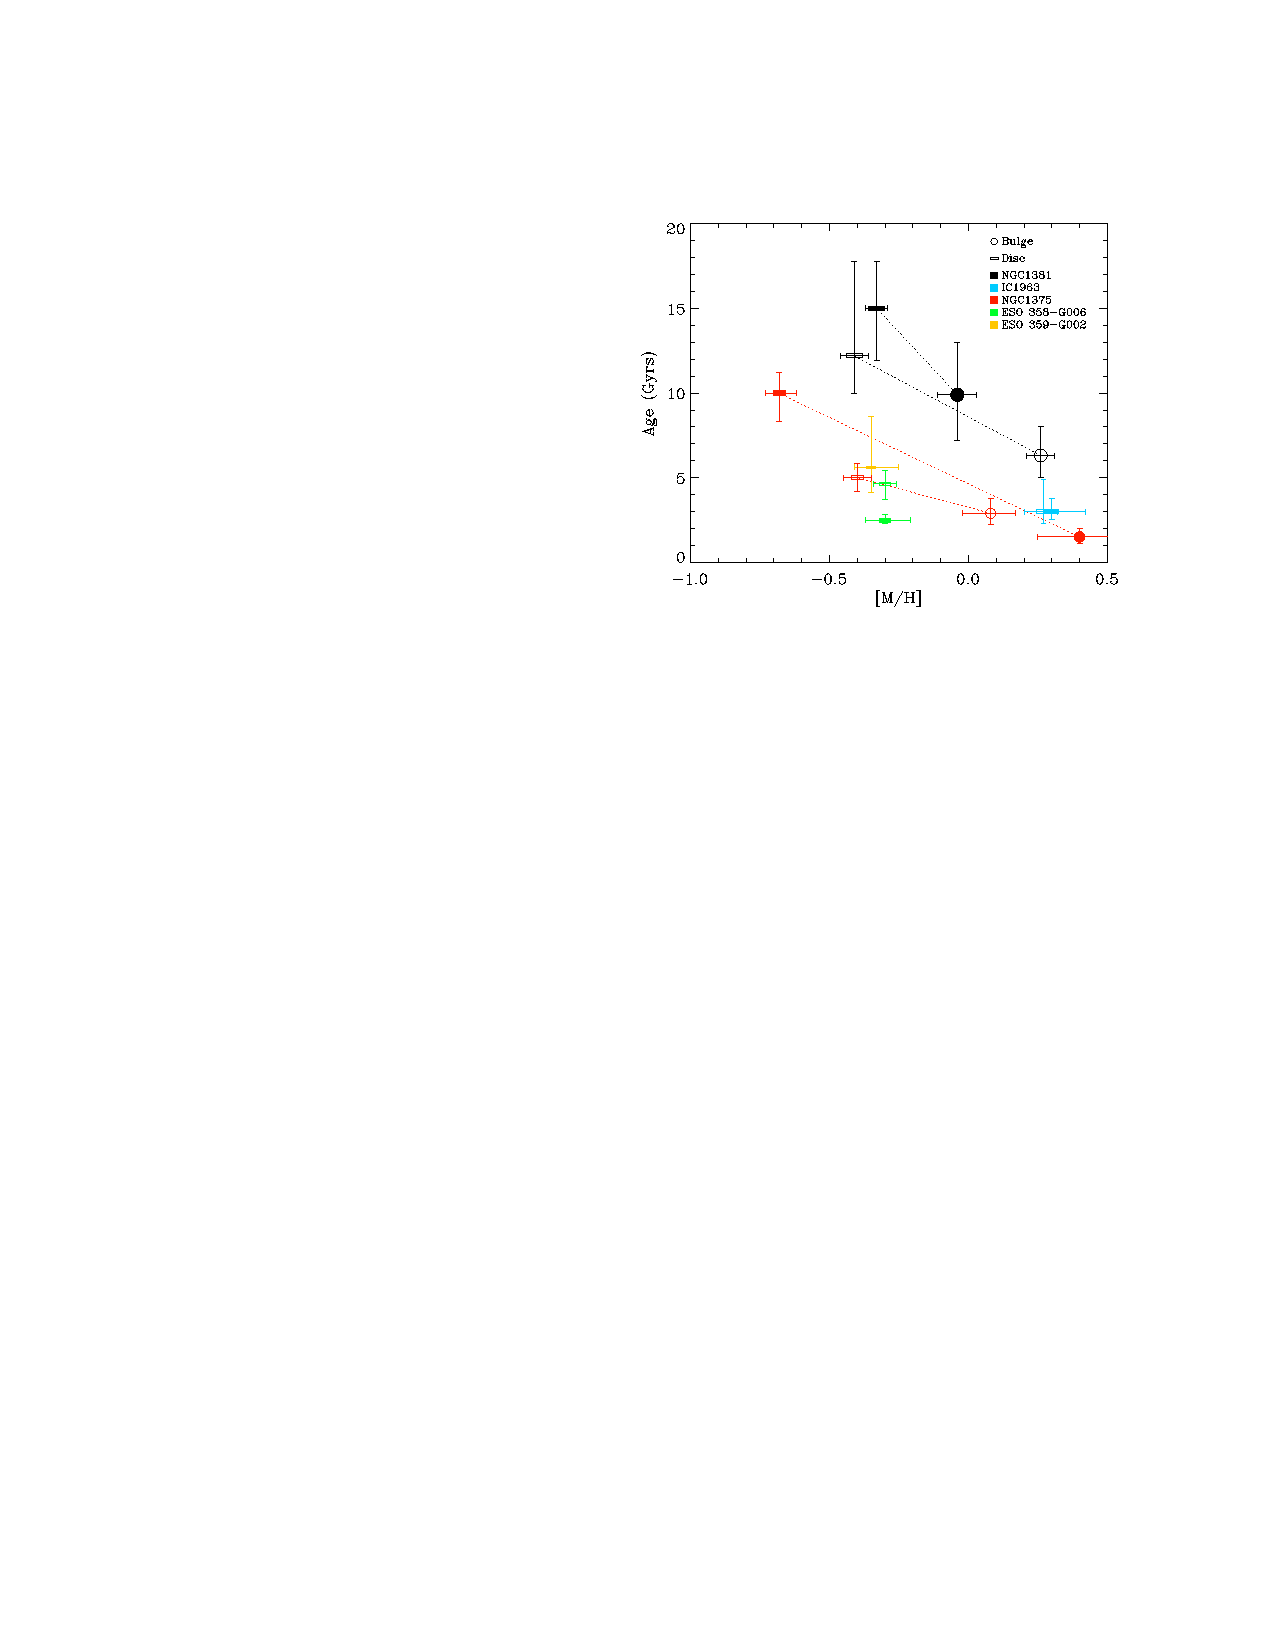
\includegraphics[width=0.9\textwidth]{figuras/johnston-pop}
	\caption[A mesma Figura que \ref{fig:populationJohnston}] {A mesma Figura que
	\ref{fig:populationJohnston}, mostrada novamente para comparar com a Figura
	\ref{fig:decompSintese}.}
	\label{fig:populationJohnston2}
\end{figure}

É interessante comparar a Figura \ref{fig:decompSintese} com o resultado de
\citet{Johnston2012}, reproduzido na Figura \ref{fig:populationJohnston2}.
Os resultados obtidos aqui, embora não tenham significância estatística, são
contrários ao resultado de \citeauthor{Johnston2012}, que obtêm, para galáxias
S0, bojos mais jovens e mais metálicos que seus discos. Tanto a idade quanto a
metalicidade que eles utilizam foram obtidos através do ajuste de duas linhas de
absorção, enquanto neste trabalho o espectro inteiro foi utilizado no ajuste de
populações estelares.

Além disso, eles trabalham com perfis unidimensionais (espectros de fenda
longa), enquanto análise feita aqui é toda em 2-d (imagens). Por fim, não é
óbvio que as galáxias de nossa amostra sejam comparáveis à da amostra de
\citeauthor{Johnston2012}. De fato, apesar de ambas amostras selecionarem
galáxias S0, as galáxias de \citeauthor{Johnston2012} parecem ser menos massivas
que as nossas. Enquanto K0858 tem magnitude absoluta na banda $B$ de $M_B = -21$
(K0592 tem medida somente na banda $V$, com $M_V = -23,6$), as de
\citeauthor{Johnston2012} $M_B$ entre $-17$ e $-19$.

Todas essas diferenças complicam a comparação dos resultados obtidos neste
trabalho com aqueles do artigo que inspirou todo esse estudo. De qualquer modo,
os experimentos aqui reportados mostram que a decomposição morfológica espectral
é um problema bastante mais delicado do que se imaginava anteriormente.


%% End of this chapter

  
  % Conclusão
  %%%%%%%%%%%%%%%%%%%%%%%%%%%%%%%%%%%%%%%%%%%%%%%%%%%%%%%%%%%%%%%%%
% Qualificacao de Doutorado / Dept Fisica, CFM, UFSC            %
% Andre@UFSC - 2015                                             %
%%%%%%%%%%%%%%%%%%%%%%%%%%%%%%%%%%%%%%%%%%%%%%%%%%%%%%%%%%%%%%%%%


%:::::::::::::::::::::::::::::::::::::::::::::::::::::::::::::::%
%                                                               %
%                          Capítulo 9                           %
%                                                               %
%:::::::::::::::::::::::::::::::::::::::::::::::::::::::::::::::%

%***************************************************************%
%                                                               %
%                           Conclusao                           %
%                                                               %
%***************************************************************%

\chapter{Conclusões e perspectivas}
\label{sec:conclusao}

O {\em survey} CALIFA observou cerca de 600 galáxias, nas configurações V500 e
V1200. Foram publicados cubos de 100 galáxias no primeiro {\em data release}, e
de 200 galáxias no segundo. Os cubos das galáxias restantes ainda estão em
processo de controle de qualidade e embargo da colaboração. Através do programa
\starlight, foram obtidos diversos parâmetros relacionados às populações
estelares componentes de cada {\em spaxel}, formando cubos de dados adicionais
ao observados, com a as propriedades físicas espacialmente resolvidas obtidas a
partir da saída do \starlight.

Neste trabalho, foi desenvolvido um programa chamado PyCASSO para organizar e
analisar estes cubos de dados. Este programa é utilizado por cerca de 10 pessoas
que estudam populações estelares na colaboração do CALIFA. Bastante atenção foi
dada à documentação (Seção \ref{sec:pycasso:Pycasso}, com o manual completo no
Apêndice \ref{apendice:manual}). Foram publicados 4 artigos que se baseiam
fortemente no uso de PyCASSO para análise e gráficos, resumidos na Seção
\ref{sec:pycasso:art} e presentes como apêndices deste trabalho (Apêndices
\ref{apendice:PaperResolving1}, \ref{apendice:PaperResolving2},
\ref{apendice:InsideOut} e \ref{apendice:RadStruct}).

Com o fim do {\em survey} CALIFA, e a liberação de todas as galáxias da amostra,
os cubos de dados de propriedades físicas poderão ser publicados. Já tivemos uma
boa experiência com a base de dados pública do \starlight
(\url{http://www.starlight.ufsc.br/}), com o resultado da síntese de população
estelar de 926246 espectros de galáxias do SDSS. Será necessária uma abordagem
diferente para o acesso aos cubos, algo que ainda precisa ser planejado e
desenvolvido.

PyCASSO já foi usado com sucesso com dados de outros {\em surveys} como o PINGS
\citep{RosalesOrtega2010}, um precursor do CALIFA, porém com até $10$ vezes mais
espectros por galáxia. MaNGA \citep{Bundy2015} está em andamento, e deverá obter
IFS de $10.000$ galáxias. Muito embora tenha um número muito maior de galáxias
do que o CALIFA, sua cobertura espacial será menor. Assim, estes {\em survey}
deverá ser complementar ao CALIFA. Testes com dados preliminares do MaNGA foram
feitos com PyCASSO, requerendo apenas pequenas modificações para que funcionem
normalmente.

É importante que PyCASSO se torne um programa modular, onde o usuário cria uma
descrição do arquivo de IFS de forma que o programa saiba como ler os dados.
Recentemente o autor deste trabalho, junto com pesquisadores do Grupo de
Astrofísica da UFSC, começou a colaborar com um novo {\em survey} chamado
Diving3D. Este {\em survey}, descrito em \citet{Ricci2014}, vai obter IFS de
quase 200 núcleos de galáxias utilizando o Telescópio Gemini. Os cubos de dados
espectrais são de uma qualidade excepcional, e já iniciamos o a adaptação de
ferramentas como o PyCASSO e o \starlight para trabalhar com esses dados. O
objetivo, do ponto de vista ferramental, é que se crie uma {\em pipeline} onde
dados como populações estelares, morfologia, etc, vão sendo adicionados de forma
incremental aos cubos, mantendo uma interface comum para análise dos dados.

Foi desenvolvida uma técnica de síntese espectral aplicada às componentes
morfológicas (bojo e disco) de galáxias. A decomposição morfológica do perfil de
brilho em uma imagem de uma galáxia é um campo de estudo bem desenvolvido, com
ferramentas bastante eficientes disponíveis na comunidade acadêmica (GALFIT,
BUDDA e IMFIT, por exemplo). A ideia aqui foi se valer destas ferramentas, junto
com PyCASSO, e realizar a decomposição para imagens em cada comprimento de onda
dos cubos de dados espectrais.

Ao fazer a decomposição morfológica em janelas estreitas de comprimento de onda,
os efeitos de cinemática precisaram ser levados em consideração. Em uma imagem
de uma galáxia, em um determinado comprimento de onda, não se observa os mesmos
processos físicos em todos os {\em pixels}. A luz de cada {\em pixel} é composta
pela luz de diversas estrelas, cada uma com uma velocidade diferente em relação
à linha de visada (e consequentemente um {\em redshift} ou {\em blueshift}
diferente), com cada {\em pixel} contendo um conjunto distinto destas
velocidades. Para mitigar este problema, a distribuição de velocidades de cada
{\em spaxel} dos cubos de dados foi determinada, de forma aproximada, por uma
velocidade sistêmica e uma dispersão de velocidades. Os {\em spaxels} foram
colocados todos no {\em rest frame}, e com a mesma dispersão de velocidade (ver
Seção \ref{sec:Decomp:cinematica} para detalhes). Isto fez com que a resolução
fosse degradada, mas garante que se observa a luz da galáxia inteira de forma
consistente.

A PSF é uma peça chave neste quebra-cabeças morfológico. Sem uma boa medida da
forma da PSF, a decomposição morfológica pode não funcionar, ou pior, gerar
resultados equivocados. No Capítulo \ref{sec:psf}, foi descrito como  a PSF do
CALIFA foi medida, um resultado que acabou sendo adotado pela colaboração,
publicado no segundo {\em data release} \citep{GarciaBenito2015}. A PSF obtida
segue um perfil de Moffat, com $\beta = 4$ e $\mathrm{FWHM}=2,9 \pm 0,3\,\arcs$.
Com esta incerteza na estimativa da largura da PSF, testes foram feitos para
determinar o efeito que um erro na PSF causa no resultado da decomposição
morfológica, apresentados na Seção \ref{sec:test:psf}. Em via de regra, a
decomposição dos espectros em componentes morfológicas, quando se utiliza a PSF
errada, apresenta artefatos como gradientes de cores e linhas espectrais
artificiais. Estes problemas parecem ser atenuados quando se utiliza os
espectros integrados das componentes morfológicas.

No Capítulo \ref{sec:Decomp} foi escolhida, dentre as galáxias do CALIFA
observadas com a configuração V500, uma amostra de 43 galáxias que foram
classificadas com boa possibilidade de serem da classe S0 (listada no Apêndice
\ref{apendice:amostra}). O objetivo era ter galáxias que pudessem ser bem
ajustadas a um modelo bojo--disco. Destas 43, 19 tinham características que não
permitiam o uso deste modelo, seja por faixas de poeira, uma das componentes
muito fraca, ou problema nos dados, entre outras coisas. Outras 15 tiveram
problema no ajuste do modelo inicial. Somente 9 galáxias tiveram um relativo
sucesso na decomposição morfológica espectral. O resultado da decomposição para
todas as 9 galáxias da amostra final é mostrado nas figuras do Apêndice
\ref{apendice:Decomp}. A galáxia K0858, classificada como S0a, foi escolhida
para uma análise mais detalhada, em parte pela sua decomposição morfológica ter
sido muito boa, e em parte por ter um bom ajuste com o \starlight.

Em K0858 verificou-se que há um gradiente espectral em alguns dos parâmetros
morfológicos, que foram ajustados levando em conta apenas informações espaciais.
Entretanto, não se pode descartar que estes gradientes, e outras características
menores observadas na dependência dos parâmetros com o comprimento de onda, não
sejam artefatos da forma como a decomposição foi feita. O teste com os erros na
PSF deixaram isto bem claro, assim como os resíduos nos espectros (vide Figura
\ref{fig:decompSpectra}). É preciso estudar a forma como os parâmetros
morfológicos deveriam variar com o comprimento de onda. Compreender a forma como
as populações estelares se distribuem nas componentes morfológicas de uma
galáxia, e como estas populações se refletem nos espectro espacialmente
resolvido da galáxia, é fundamental para poder fazer uma decomposição
morfológica que leve em conta informações das regiões vizinhas no espectro.

A síntese de populações estelares foi realizada com sucesso apenas em K0592
(classificada como E0), e K0858. O ajuste dos espectros e as propriedades
físicas, para todas as 9 galáxias da amostra, estão disponíveis no Apêndice
\ref{apendice:Decomp}. Apenas K0592 e K0858 tiveram um resíduo no ajuste do
\starlight pequeno o bastante para poderem ter as propriedades físicas obtidas
para seus bojos e discos levadas a sério. A Figura \ref{fig:decompSintese}
mostra idade e metalicidade estelar médias para as componentes das duas
galáxias, calculados sobre os espectros integrados. Esta figura indica que os
bojos apresentam populações mais velhas e menos metálicas, enquanto os discos
apresentam populações mais jovens e mais metálicas, em relação ao espectro
observado.

Um estudo que poderia ser feito com os resultados da síntese de populações
aplicados à decomposição morfológica espectral é medir a densidade superficial
de massa estelar do disco, que fica normalmente ofuscado pelo bojo nas regiões
centrais. O objetivo é verificar previsão de \citet{Freeman1970}, que diz que a
densidade superficial de massa do núcleo dos discos de galáxias é sempre o
mesmo, independente do tipo morfológico e do perfil de massa que a galáxia
tenha. Todavia, a síntese de populações espacialmente resolvida não é muito
robusta da forma como é feita aqui, como visto na Figura
\ref{fig:decompSinteseRadprof}. Entre as prováveis causas está a degenerescência
no modelo bojo--disco, com 7 parâmetros livres. Deixar parâmetros como P.A. e
$\epsilon$ fixos pode ajudar, mas isso requer testes.

Muitos problemas podem ter sido causados pela forma como se trata a cinemática.
Talvez seja preciso fazer testes com modelos dinâmicos simples de galáxias para
verificar se a abordagem utilizada é mesmo adequada. Outra alternativa seria
fazer a decomposição de forma iterativa. Depois de ter determinado as
componentes morfológicas, utilizar este conhecimento para tentar medir a
cinemática das duas componentes nos dados originais, e tentar fazer uma
correção melhor, repetindo a decomposição. Não é óbvio, entretanto, que esta
abordagem vá realmente convergir, ou mesmo se é factível computacionalmente.

Mesmo com todos estes problemas em potencial, o passo lógico seguinte é tentar
aplicar o ajuste a galáxias espirais. A própria K0858 apresenta um resíduo no
ajuste morfológico que parece um braço espiral (ver Figura
\ref{fig:decompImages:K0858}). Os braços espirais têm um papel importante na
formação estelar, e com esta abordagem pode-se tentar obter o histórico de
formação estelar nestas regiões. Também pode-se tentar utilizar um outro modelo
morfológico para ajustar galáxias com um grande ângulo de inclinação. Com mais
galáxias, seria possível aplicar o estudo a uma boa fração da amostra do CALIFA,
e obter uma melhor estatística.

% End of this chapter

  
  \appendix
  
  % Amostra da decomposição
  %%%%%%%%%%%%%%%%%%%%%%%%%%%%%%%%%%%%%%%%%%%%%%%%%%%%%%%%%%%%%%%%%
% Qualificacao de Doutorado / Dept Fisica, CFM, UFSC            %
% Andre@UFSC - 2013                                             %
%%%%%%%%%%%%%%%%%%%%%%%%%%%%%%%%%%%%%%%%%%%%%%%%%%%%%%%%%%%%%%%%%


%:::::::::::::::::::::::::::::::::::::::::::::::::::::::::::::::%
%                                                               %
%                       Anexo: Amostra                          %
%                                                               %
%:::::::::::::::::::::::::::::::::::::::::::::::::::::::::::::::%

\chapter{Amostra para decomposição morfológica espectral}
\label{apendice:amostra}



\begin{longtable}{ l l r r r r l }
%\setlength{\tabcolsep}{1cm}
{{\bfseries \tablename\ \thetable{}}}
\\
\hline \textbf{ID} & \textbf{Nome} & \textbf{Classe} & \textbf{Mín.} &
\textbf{Máx.} & $\epsilon$ &
\textbf{Obs.} \\ \hline
\endfirsthead

\multicolumn{3}{c}%
{{\bfseries \tablename\ \thetable{} -- continuada da página anterior}}
\\
\hline \textbf{ID} & \textbf{Nome} & \textbf{Classe} & \textbf{Mín.} &
\textbf{Máx.} & $\epsilon$ &
\textbf{Obs.} \\ \hline
\endhead

\multicolumn{7}{r}{{Continua na próxima página}} \\
\hline
\endfoot

\hline
\endlastfoot

K0018 & NGC 0155  &  1 (E1)  & 0 (E0) &  8 (S0)  & $0,22$ & - \\
K0020 & NGC 0160  & 10 (Sa)  & 8 (S0) & 13 (Sbc) & $0,37$ & Disco fraco \\
K0044 & NGC 0499  &  5 (E5)  & 2 (E2) &  8 (S0)  & $0,39$ & Ajuste ruim \\
K0046 & NGC 0504  &  8 (S0)  & 7 (E7) &  8 (S0)  & $0,47$ & Inclinada \\
K0051 & NGC 0529  &  4 (E4)  & 3 (E3) &  8 (S0)  & $0,14$ & Disco fraco \\
K0072 & NGC 0774  &  8 (S0)  & 6 (E6) &  8 (S0)  & $0,28$ & Disco fraco \\
K0087 & NGC 0932  &  9 (S0a) & 8 (S0) & 10 (Sa)  & $0,04$ & Braço espiral \\
K0100 & NGC 1056  & 10 (Sa)  & 8 (S0) & 11 (Sab) & $0,43$ & Faixa de poeira \\
K0119 & NGC 1167  &  8 (S0)  & 7 (E7) & 10 (Sa)  & $0,19$ & Ajuste ruim \\
K0127 & NGC 1349  &  6 (E6)  & 0 (E0) & 10 (Sa)  & $0,11$ & - \\
K0160 & NGC 2476  &  6 (E6)  & 3 (E3) &  8 (S0)  & $0,31$ & Ajuste ruim \\
K0279 & NGC 2918  &  6 (E6)  & 4 (E4) &  8 (S0)  & $0,29$ & Ajuste ruim \\
K0311 & NGC 3106  & 11 (Sab) & 8 (S0) & 19 (Ir)  & $0,07$ & Ajuste ruim \\
K0341 & UGC 05771 &  6 (E6)  & 4 (E4) &  8 (S0)  & $0,29$ & Ajuste ruim \\
K0548 & NGC 4470  & 14 (Sc)  & 5 (E5) & 19 (Ir)  & $0,34$ & Irregular \\
K0592 & NGC 4874  &  0 (E0)  & 0 (E0) &  8 (S0)  & $0,12$ & - \\
K0602 & NGC 4956  &  1 (E1)  & 0 (E0) &  8 (S0)  & $0,14$ & - \\
K0607 & UGC 08234 &  8 (S0)  & 6 (E6) &  8 (S0)  & $0,37$ & Ajuste ruim \\
K0612 & NGC 5029  &  6 (E6)  & 4 (E4) &  8 (S0)  & $0,32$ & Ajuste ruim \\
K0633 & NGC 5216  &  0 (E0)  & 0 (E0) &  8 (S0)  & $0,09$ & Disco fraco \\
K0708 & NGC 5485  &  5 (E5)  & 1 (E1) &  8 (S0)  & $0,19$ & Faixa de poeira \\
K0744 & NGC 5631  &  8 (S0)  & 1 (E1) &  8 (S0)  & $0,11$ & Faixa de poeira \\
K0778 & NGC 5784  &  8 (S0)  & 1 (E1) &  8 (S0)  & $0,19$ & Faixa de poeira \\
K0780 & NGC 5797  &  7 (E7)  & 4 (E4) &  8 (S0)  & $0,35$ & Ajuste ruim \\
K0814 & UGC 10097 &  5 (E5)  & 1 (E1) &  8 (S0)  & $0,26$ & Ajuste ruim \\
K0816 & NGC 6021  &  5 (E5)  & 3 (E3) &  8 (S0)  & $0,22$ & Ajuste ruim \\
K0822 & UGC 10205 &  9 (S0a) & 8 (S0) & 10 (Sa)  & $0,42$ & Faixa de poeira \\
K0832 & NGC 6146  &  5 (E5)  & 3 (E3) &  8 (S0)  & $0,23$ & - \\
K0840 & NGC 6173  &  6 (E6)  & 3 (E3) &  8 (S0)  & $0,35$ & Ajuste ruim \\
K0846 & UGC 10695 &  5 (E5)  & 2 (E2) &  8 (S0)  & $0,33$ & - \\
K0850 & NGC 6314  & 11 (Sab) & 8 (S0) & 14 (Sc)  & $0,49$ & Faixa de poeira \\
K0851 & NGC 6338  &  5 (E5)  & 1 (E1) &  8 (S0)  & $0,34$ & - \\
K0858 & UGC 10905 &  9 (S0a) & 7 (E7) & 11 (Sab) & $0,47$ & - \\
K0874 & NGC 7025  &  9 (S0a) & 8 (S0) & 10 (Sa)  & $0,28$ & Poucos {\em spaxels} \\
K0875 & UGC 11694 &  9 (S0a) & 8 (S0) & 10 (Sa)  & $0,23$ & Faixa de poeira \\
K0900 & NGC 7550  &  4 (E4)  & 0 (E0) &  8 (S0)  & $0,08$ & Ajuste ruim \\
K0908 & NGC 7611  &  8 (S0)  & 6 (E6) &  8 (S0)  & $0,50$ & Inclinada \\
K0912 & NGC 7623  &  8 (S0)  & 8 (S0) &  8 (S0)  & $0,29$ & - \\
K0913 & NGC 7625  & 10 (Sa)  & 0 (E0) & 19 (Ir)  & $0,22$ & Faixa de poeira \\
K0916 & NGC 7671  &  8 (S0)  & 7 (E7) &  8 (S0)  & $0,35$ & Ajuste ruim \\
K0917 & NGC 7683  &  8 (S0)  & 6 (E6) &  8 (S0)  & $0,38$ & Ajuste ruim \\
K0923 & NGC 7711  &  7 (E7)  & 4 (E4) &  8 (S0)  & $0,47$ & Disco fraco \\
K0925 & NGC 7722  & 11 (Sab) & 3 (E3) & 19 (Ir)  & $0,13$ & Faixa de poeira \\
\hline
\caption[Amostra selecionada para decomposição morfológica espectral.]
{Amostra selecionada para decomposição morfológica espectral.}
\label{tab:DecompSample}
\end{longtable}


% End of this chapter


  % Plots da decomposição e sintese
  %%%%%%%%%%%%%%%%%%%%%%%%%%%%%%%%%%%%%%%%%%%%%%%%%%%%%%%%%%%%%%%%%
% Qualificacao de Doutorado / Dept Fisica, CFM, UFSC            %
% Andre@UFSC - 2015                                             %
%%%%%%%%%%%%%%%%%%%%%%%%%%%%%%%%%%%%%%%%%%%%%%%%%%%%%%%%%%%%%%%%%


%:::::::::::::::::::::::::::::::::::::::::::::::::::::::::::::::%
%                                                               %
%                       Anexo: Decomposição                     %
%                                                               %
%:::::::::::::::::::::::::::::::::::::::::::::::::::::::::::::::%

\chapter{Decomposição morfológica espectral e síntese de populações estelares
da amostra final}
\label{apendice:Decomp}


%***************************************************************%
%                                                               %
%                           K0018                               %
%                                                               %
%***************************************************************%

\section{K0018 (NGC 0155)}
\label{apendice:Decomp:K0018}

\begin{itemize}
  \item Galáxia NGC 0155
  \item Tipo morfológico: E1 (mín. E0, máx. S0)
  \item Magnitude absoluta na banda $r$: $-21,85$
  \item Elipticidade: $0,22$
\end{itemize}

\begin{figure}
	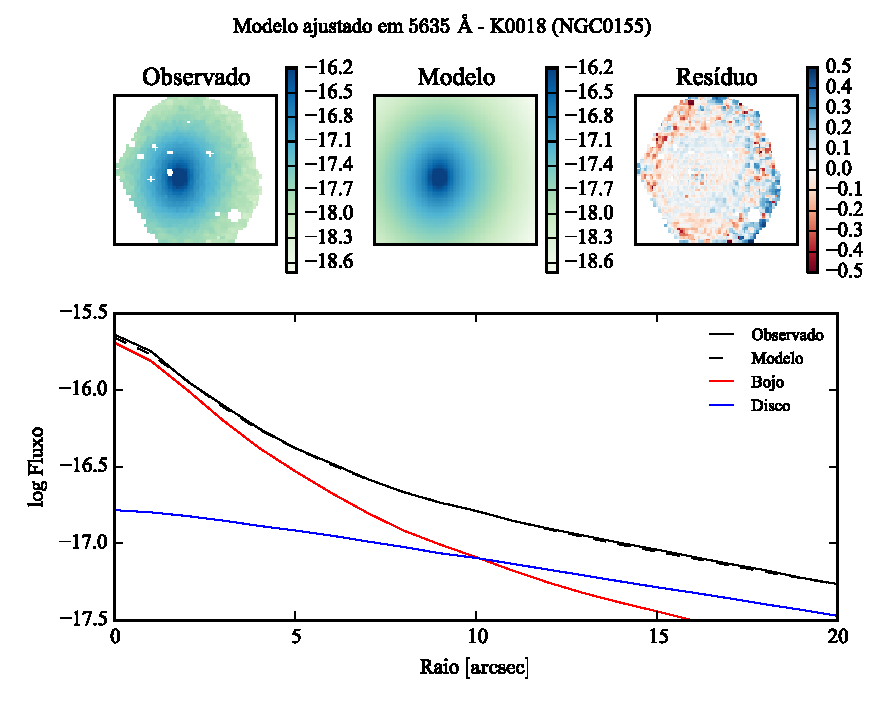
\includegraphics[page=1]{figuras-decomp/K0018_sample006a}
	\caption[Ajuste morfológico em $5635\,\angstrom$ de K0018 (NGC 0155)]
	{Acima: imagens observada, modelada e resíduo, do fluxo em $5635\,\angstrom$
	para K0018 (NGC 0155). Abaixo: perfis radiais, obtidos pela média do fluxo em
	anéis elípticos nas imagens. O fluxo observado é representado pela linha preta
	sólida. O melhor ajuste é representado pela linha preta tracejada. O bojo e o
	disco que compõe o modelo são mostrados em vermelho e azul, respectivamente.}
	\label{fig:decompRadprof:K0018}
\end{figure}

\begin{figure}
	\includegraphics[page=2]{figuras-decomp/K0018_sample006a}
	\caption[Parâmetros morfológicos em função do comprimento de onda de K0018
	(NGC 0155)]
	{Parâmetros morfológicos em função do comprimento de onda para
	K0018 (NGC 0155). Regiões em rosa representam comprimentos de onda onde a
	decomposição falhou. Regiões em cinza foram mascaradas antes de iniciar a
	decomposição. Pontos azuis indicam o primeiro passo da decomposição, em caixas
	de $100\,\angstrom$.}
	\label{fig:decompParams:K0018}
\end{figure}

\begin{figure}
	\includegraphics[page=3]{figuras-decomp/K0018_sample006a}
	\caption[Imagens em $5635\,\angstrom$ das componentes morfológicas de K0018
	(NGC 0155)]
	{Imagens em $5635\,\angstrom$ das componentes morfológicas de K0018
	(NGC 0155).}
	\label{fig:decompImages:K0018}
\end{figure}

\begin{figure}
	\includegraphics[page=4]{figuras-decomp/K0018_sample006a}
	\caption[Espectro das componentes morfológicas de K0018 (NGC 0155)]
	{Espectro das componentes morfológicas de K0018 (NGC 0155),
	observado (preto), bojo (vermelho), disco (azul) e resíduo (magenta). Acima:
	Espectro do {\em spaxel} nuclear da galáxia. Meio: Espectro em um {\em spaxel}
	a uma distância de $r_e$ do núcleo. Abaixo: Espectro integrado espacialmente.}
	\label{fig:decompSpectra:K0018}
\end{figure}

\begin{figure}
	\includegraphics[page=5]{figuras-decomp/K0018_sample006a}
	\caption[Perfis radiais para diversos comprimentos de onda de K0018 (NGC 0155)]
	{Perfis radiais para diversos comprimentos de onda de K0018 (NGC 0155).}
	\label{fig:decompRadprofSpec:K0018}
\end{figure}

\begin{figure}
	\includegraphics[page=1]{figuras/sample006a_synthesis}
	\caption[Espectros ajustados com \starlight das componentes morfológicas de
	K0018 (NGC 0155)]
	{Acima: Espectros integrados das componentes morfológicas de
	K0018 (NGC 0155), ajustados com \starlight. Em preto, espectro observado. Em
	vermelho, e azul, as componentes bojo e disco. Em linhas de cor clara, o
	espectro ajustado pelo \starlight. Abaixo: Resíduo dos espectros (observado
	menos sintético, divididos pelo observado).}
	\label{fig:decompSintese:K0018}
\end{figure}

\begin{figure}
	\includegraphics[page=2]{figuras/sample006a_synthesis}
	\caption[Propriedades físicas das componentes morfológicas de K0018 (NGC 0155)]
	{Perfil radial de propriedades físicas das componentes morfológicas de
	K0018 (NGC 0155), obtidos através do \starlight. As linhas contínuas
	representam as propriedades obtidas utilizando espectros espacialmente
	resolvidos. As linhas tracejadas representam as propriedades obtidas utilizando
	os espectros integrados. Em preto, espectro observado. Em vermelho, e azul, as
	componentes bojo e disco. Acima, à esquerda: idade estelar média ponderada pela
	luminosidade. Acima, à direita: atenuação por poeira, na banda $V$. Abaixo, à
	esquerda: metalicidade estelar média, ponderada pela massa. Abaixo, à direita:
	densidade superficial de massa estelar. As frações de massa e luminosidade
	entre as componentes e a total (obtida do espectro observado) é mostrada no
	painel inferior, à direita.}
	\label{fig:decompSinteseRadprof:K0018}
\end{figure}

\FloatBarrier

%***************************************************************%
%                                                               %
%                           K0127                               %
%                                                               %
%***************************************************************%

\section{K0127 (NGC 1349)}
\label{apendice:Decomp:K0127}

\begin{itemize}
  \item Galáxia NGC 1349
  \item Tipo morfológico: E6 (mín. E0, máx. Sa)
  \item Magnitude absoluta na banda $r$: $-22,15$
  \item Elipticidade: $0,11$
\end{itemize}

\begin{figure}
	\includegraphics[page=1]{figuras-decomp/K0127_sample006a}
	\caption[Ajuste morfológico em $5635\,\angstrom$ de K0127 (NGC 1349)]
	{Acima: imagens observada, modelada e resíduo, do fluxo em $5635\,\angstrom$
	para K0127 (NGC 1349). Abaixo: perfis radiais, obtidos pela média do fluxo em
	anéis elípticos nas imagens. O fluxo observado é representado pela linha preta
	sólida. O melhor ajuste é representado pela linha preta tracejada. O bojo e o
	disco que compõe o modelo são mostrados em vermelho e azul, respectivamente.}
	\label{fig:decompRadprof:K0127}
\end{figure}

\begin{figure}
	\includegraphics[page=2]{figuras-decomp/K0127_sample006a}
	\caption[Parâmetros morfológicos em função do comprimento de onda de K0127
	(NGC 1349)]
	{Parâmetros morfológicos em função do comprimento de onda para
	K0127 (NGC 1349). Regiões em rosa representam comprimentos de onda onde a
	decomposição falhou. Regiões em cinza foram mascaradas antes de iniciar a
	decomposição. Pontos azuis indicam o primeiro passo da decomposição, em caixas
	de $100\,\angstrom$.}
	\label{fig:decompParams:K0127}
\end{figure}

\begin{figure}
	\includegraphics[page=3]{figuras-decomp/K0127_sample006a}
	\caption[Imagens em $5635\,\angstrom$ das componentes morfológicas de K0127
	(NGC 1349)]
	{Imagens em $5635\,\angstrom$ das componentes morfológicas de K0127
	(NGC 1349).}
	\label{fig:decompImages:K0127}
\end{figure}

\begin{figure}
	\includegraphics[page=4]{figuras-decomp/K0127_sample006a}
	\caption[Espectro das componentes morfológicas de K0127 (NGC 1349)]
	{Espectro das componentes morfológicas de K0127 (NGC 1349),
	observado (preto), bojo (vermelho), disco (azul) e resíduo (magenta). Acima:
	Espectro do {\em spaxel} nuclear da galáxia. Meio: Espectro em um {\em spaxel}
	a uma distância de $r_e$ do núcleo. Abaixo: Espectro integrado espacialmente.}
	\label{fig:decompSpectra:K0127}
\end{figure}

\begin{figure}
	\includegraphics[page=5]{figuras-decomp/K0127_sample006a}
	\caption[Perfis radiais para diversos comprimentos de onda de K0127 (NGC 1349)]
	{Perfis radiais para diversos comprimentos de onda de K0127 (NGC 1349).}
	\label{fig:decompRadprofSpec:K0127}
\end{figure}

\begin{figure}
	\includegraphics[page=3]{figuras/sample006a_synthesis}
	\caption[Espectros ajustados com \starlight das componentes morfológicas de
	K0127 (NGC 1349)]
	{Acima: Espectros integrados das componentes morfológicas de
	K0127 (NGC 1349), ajustados com \starlight. Em preto, espectro observado. Em
	vermelho, e azul, as componentes bojo e disco. Em linhas de cor clara, o
	espectro ajustado pelo \starlight. Abaixo: Resíduo dos espectros (observado
	menos sintético, divididos pelo observado).}
	\label{fig:decompSintese:K0127}
\end{figure}

\begin{figure}
	\includegraphics[page=4]{figuras/sample006a_synthesis}
	\caption[Propriedades físicas das componentes morfológicas de K0127 (NGC 1349)]
	{Perfil radial de propriedades físicas das componentes morfológicas de
	K0127 (NGC 1349), obtidos através do \starlight. As linhas contínuas
	representam as propriedades obtidas utilizando espectros espacialmente
	resolvidos. As linhas tracejadas representam as propriedades obtidas utilizando
	os espectros integrados. Em preto, espectro observado. Em vermelho, e azul, as
	componentes bojo e disco. Acima, à esquerda: idade estelar média ponderada pela
	luminosidade. Acima, à direita: atenuação por poeira, na banda $V$. Abaixo, à
	esquerda: metalicidade estelar média, ponderada pela massa. Abaixo, à direita:
	densidade superficial de massa estelar. As frações de massa e luminosidade
	entre as componentes e a total (obtida do espectro observado) é mostrada no
	painel inferior, à direita.}
	\label{fig:decompSinteseRadprof:K0127}
\end{figure}

\FloatBarrier

%***************************************************************%
%                                                               %
%                           K0592                               %
%                                                               %
%***************************************************************%

\section{K0592 (NGC 4874)}
\label{apendice:Decomp:K0592}

\begin{itemize}
  \item Galáxia NGC 4874
  \item Tipo morfológico: E0 (mín. E0, máx. S0)
  \item Magnitude absoluta na banda $r$: $-22,67$
  \item Elipticidade: $0,12$
\end{itemize}

\begin{figure}
	\includegraphics[page=1]{figuras-decomp/K0592_sample006a}
	\caption[Ajuste morfológico em $5635\,\angstrom$ de K0592 (NGC 4874)]
	{Acima: imagens observada, modelada e resíduo, do fluxo em $5635\,\angstrom$
	para K0592 (NGC 4874). Abaixo: perfis radiais, obtidos pela média do fluxo em
	anéis elípticos nas imagens. O fluxo observado é representado pela linha preta
	sólida. O melhor ajuste é representado pela linha preta tracejada. O bojo e o
	disco que compõe o modelo são mostrados em vermelho e azul, respectivamente.}
	\label{fig:decompRadprof:K0592}
\end{figure}

\begin{figure}
	\includegraphics[page=2]{figuras-decomp/K0592_sample006a}
	\caption[Parâmetros morfológicos em função do comprimento de onda de K0592
	(NGC 4874)]
	{Parâmetros morfológicos em função do comprimento de onda para
	K0592 (NGC 4874). Regiões em rosa representam comprimentos de onda onde a
	decomposição falhou. Regiões em cinza foram mascaradas antes de iniciar a
	decomposição. Pontos azuis indicam o primeiro passo da decomposição, em caixas
	de $100\,\angstrom$.}
	\label{fig:decompParams:K0592}
\end{figure}

\begin{figure}
	\includegraphics[page=3]{figuras-decomp/K0592_sample006a}
	\caption[Imagens em $5635\,\angstrom$ das componentes morfológicas de K0592
	(NGC 4874)]
	{Imagens em $5635\,\angstrom$ das componentes morfológicas de K0592
	(NGC 4874).}
	\label{fig:decompImages:K0592}
\end{figure}

\begin{figure}
	\includegraphics[page=4]{figuras-decomp/K0592_sample006a}
	\caption[Espectro das componentes morfológicas de K0592 (NGC 4874)]
	{Espectro das componentes morfológicas de K0592 (NGC 4874),
	observado (preto), bojo (vermelho), disco (azul) e resíduo (magenta). Acima:
	Espectro do {\em spaxel} nuclear da galáxia. Meio: Espectro em um {\em spaxel}
	a uma distância de $r_e$ do núcleo. Abaixo: Espectro integrado espacialmente.}
	\label{fig:decompSpectra:K0592}
\end{figure}

\begin{figure}
	\includegraphics[page=5]{figuras-decomp/K0592_sample006a}
	\caption[Perfis radiais para diversos comprimentos de onda de K0592 (NGC 4874)]
	{Perfis radiais para diversos comprimentos de onda de K0592 (NGC 4874).}
	\label{fig:decompRadprofSpec:K0592}
\end{figure}

\begin{figure}
	\includegraphics[page=5]{figuras/sample006a_synthesis}
	\caption[Espectros ajustados com \starlight das componentes morfológicas de
	K0592 (NGC 4874)]
	{Acima: Espectros integrados das componentes morfológicas de
	K0592 (NGC 4874), ajustados com \starlight. Em preto, espectro observado. Em
	vermelho, e azul, as componentes bojo e disco. Em linhas de cor clara, o
	espectro ajustado pelo \starlight. Abaixo: Resíduo dos espectros (observado
	menos sintético, divididos pelo observado).}
	\label{fig:decompSintese:K0592}
\end{figure}

\begin{figure}
	\includegraphics[page=6]{figuras/sample006a_synthesis}
	\caption[Propriedades físicas das componentes morfológicas de K0592 (NGC 4874)]
	{Perfil radial de propriedades físicas das componentes morfológicas de
	K0592 (NGC 4874), obtidos através do \starlight. As linhas contínuas
	representam as propriedades obtidas utilizando espectros espacialmente
	resolvidos. As linhas tracejadas representam as propriedades obtidas utilizando
	os espectros integrados. Em preto, espectro observado. Em vermelho, e azul, as
	componentes bojo e disco. Acima, à esquerda: idade estelar média ponderada pela
	luminosidade. Acima, à direita: atenuação por poeira, na banda $V$. Abaixo, à
	esquerda: metalicidade estelar média, ponderada pela massa. Abaixo, à direita:
	densidade superficial de massa estelar. As frações de massa e luminosidade
	entre as componentes e a total (obtida do espectro observado) é mostrada no
	painel inferior, à direita.}
	\label{fig:decompSinteseRadprof:K0592}
\end{figure}

\FloatBarrier

%***************************************************************%
%                                                               %
%                           K0602                               %
%                                                               %
%***************************************************************%

\section{K0602 (NGC 4956)}
\label{apendice:Decomp:K0602}

\begin{itemize}
  \item Galáxia NGC 4956
  \item Tipo morfológico: E1 (mín. E0, máx. S0)
  \item Magnitude absoluta na banda $r$: $-21,97$
  \item Elipticidade: $0,14$
\end{itemize}

\begin{figure}
	\includegraphics[page=1]{figuras-decomp/K0602_sample006a}
	\caption[Ajuste morfológico em $5635\,\angstrom$ de K0602 (NGC 4956)]
	{Acima: imagens observada, modelada e resíduo, do fluxo em $5635\,\angstrom$
	para K0602 (NGC 4956). Abaixo: perfis radiais, obtidos pela média do fluxo em
	anéis elípticos nas imagens. O fluxo observado é representado pela linha preta
	sólida. O melhor ajuste é representado pela linha preta tracejada. O bojo e o
	disco que compõe o modelo são mostrados em vermelho e azul, respectivamente.}
	\label{fig:decompRadprof:K0602}
\end{figure}

\begin{figure}
	\includegraphics[page=2]{figuras-decomp/K0602_sample006a}
	\caption[Parâmetros morfológicos em função do comprimento de onda de K0602
	(NGC 4956)]
	{Parâmetros morfológicos em função do comprimento de onda para
	K0602 (NGC 4956). Regiões em rosa representam comprimentos de onda onde a
	decomposição falhou. Regiões em cinza foram mascaradas antes de iniciar a
	decomposição. Pontos azuis indicam o primeiro passo da decomposição, em caixas
	de $100\,\angstrom$.}
	\label{fig:decompParams:K0602}
\end{figure}

\begin{figure}
	\includegraphics[page=3]{figuras-decomp/K0602_sample006a}
	\caption[Imagens em $5635\,\angstrom$ das componentes morfológicas de K0602
	(NGC 4956)]
	{Imagens em $5635\,\angstrom$ das componentes morfológicas de K0602
	(NGC 4956).}
	\label{fig:decompImages:K0602}
\end{figure}

\begin{figure}
	\includegraphics[page=4]{figuras-decomp/K0602_sample006a}
	\caption[Espectro das componentes morfológicas de K0602 (NGC 4956)]
	{Espectro das componentes morfológicas de K0602 (NGC 4956),
	observado (preto), bojo (vermelho), disco (azul) e resíduo (magenta). Acima:
	Espectro do {\em spaxel} nuclear da galáxia. Meio: Espectro em um {\em spaxel}
	a uma distância de $r_e$ do núcleo. Abaixo: Espectro integrado espacialmente.}
	\label{fig:decompSpectra:K0602}
\end{figure}

\begin{figure}
	\includegraphics[page=5]{figuras-decomp/K0602_sample006a}
	\caption[Perfis radiais para diversos comprimentos de onda de K0602 (NGC 4956)]
	{Perfis radiais para diversos comprimentos de onda de K0602 (NGC 4956).}
	\label{fig:decompRadprofSpec:K0602}
\end{figure}

\begin{figure}
	\includegraphics[page=7]{figuras/sample006a_synthesis}
	\caption[Espectros ajustados com \starlight das componentes morfológicas de
	K0602 (NGC 4956)]
	{Acima: Espectros integrados das componentes morfológicas de
	K0602 (NGC 4956), ajustados com \starlight. Em preto, espectro observado. Em
	vermelho, e azul, as componentes bojo e disco. Em linhas de cor clara, o
	espectro ajustado pelo \starlight. Abaixo: Resíduo dos espectros (observado
	menos sintético, divididos pelo observado).}
	\label{fig:decompSintese:K0602}
\end{figure}

\begin{figure}
	\includegraphics[page=8]{figuras/sample006a_synthesis}
	\caption[Propriedades físicas das componentes morfológicas de K0602 (NGC 4956)]
	{Perfil radial de propriedades físicas das componentes morfológicas de
	K0602 (NGC 4956), obtidos através do \starlight. As linhas contínuas
	representam as propriedades obtidas utilizando espectros espacialmente
	resolvidos. As linhas tracejadas representam as propriedades obtidas utilizando
	os espectros integrados. Em preto, espectro observado. Em vermelho, e azul, as
	componentes bojo e disco. Acima, à esquerda: idade estelar média ponderada pela
	luminosidade. Acima, à direita: atenuação por poeira, na banda $V$. Abaixo, à
	esquerda: metalicidade estelar média, ponderada pela massa. Abaixo, à direita:
	densidade superficial de massa estelar. As frações de massa e luminosidade
	entre as componentes e a total (obtida do espectro observado) é mostrada no
	painel inferior, à direita.}
	\label{fig:decompSinteseRadprof:K0602}
\end{figure}

\FloatBarrier

%***************************************************************%
%                                                               %
%                           K0832                               %
%                                                               %
%***************************************************************%

\section{K0832 (NGC 6146)}
\label{apendice:Decomp:K0832}

\begin{itemize}
  \item Galáxia NGC 6146
  \item Tipo morfológico: E5 (mín. E3, máx. S0)
  \item Magnitude absoluta na banda $r$: $-22,94$
  \item Elipticidade: $0,23$
\end{itemize}


\begin{figure}
	\includegraphics[page=1]{figuras-decomp/K0832_sample006a}
	\caption[Ajuste morfológico em $5635\,\angstrom$ de K0832 (NGC 6146)]
	{Acima: imagens observada, modelada e resíduo, do fluxo em $5635\,\angstrom$
	para K0832 (NGC 6146). Abaixo: perfis radiais, obtidos pela média do fluxo em
	anéis elípticos nas imagens. O fluxo observado é representado pela linha preta
	sólida. O melhor ajuste é representado pela linha preta tracejada. O bojo e o
	disco que compõe o modelo são mostrados em vermelho e azul, respectivamente.}
	\label{fig:decompRadprof:K0832}
\end{figure}

\begin{figure}
	\includegraphics[page=2]{figuras-decomp/K0832_sample006a}
	\caption[Parâmetros morfológicos em função do comprimento de onda de K0832
	(NGC 6146)]
	{Parâmetros morfológicos em função do comprimento de onda para
	K0832 (NGC 6146). Regiões em rosa representam comprimentos de onda onde a
	decomposição falhou. Regiões em cinza foram mascaradas antes de iniciar a
	decomposição. Pontos azuis indicam o primeiro passo da decomposição, em caixas
	de $100\,\angstrom$.}
	\label{fig:decompParams:K0832}
\end{figure}

\begin{figure}
	\includegraphics[page=3]{figuras-decomp/K0832_sample006a}
	\caption[Imagens em $5635\,\angstrom$ das componentes morfológicas de K0832
	(NGC 6146)]
	{Imagens em $5635\,\angstrom$ das componentes morfológicas de K0832
	(NGC 6146).}
	\label{fig:decompImages:K0832}
\end{figure}

\begin{figure}
	\includegraphics[page=4]{figuras-decomp/K0832_sample006a}
	\caption[Espectro das componentes morfológicas de K0832 (NGC 6146)]
	{Espectro das componentes morfológicas de K0832 (NGC 6146),
	observado (preto), bojo (vermelho), disco (azul) e resíduo (magenta). Acima:
	Espectro do {\em spaxel} nuclear da galáxia. Meio: Espectro em um {\em spaxel}
	a uma distância de $r_e$ do núcleo. Abaixo: Espectro integrado espacialmente.}
	\label{fig:decompSpectra:K0832}
\end{figure}

\begin{figure}
	\includegraphics[page=5]{figuras-decomp/K0832_sample006a}
	\caption[Perfis radiais para diversos comprimentos de onda de K0832 (NGC 6146)]
	{Perfis radiais para diversos comprimentos de onda de K0832 (NGC 6146).}
	\label{fig:decompRadprofSpec:K0832}
\end{figure}

\begin{figure}
	\includegraphics[page=9]{figuras/sample006a_synthesis}
	\caption[Espectros ajustados com \starlight das componentes morfológicas de
	K0832 (NGC 6146)]
	{Acima: Espectros integrados das componentes morfológicas de
	K0832 (NGC 6146), ajustados com \starlight. Em preto, espectro observado. Em
	vermelho, e azul, as componentes bojo e disco. Em linhas de cor clara, o
	espectro ajustado pelo \starlight. Abaixo: Resíduo dos espectros (observado
	menos sintético, divididos pelo observado).}
	\label{fig:decompSintese:K0832}
\end{figure}

\begin{figure}
	\includegraphics[page=10]{figuras/sample006a_synthesis}
	\caption[Propriedades físicas das componentes morfológicas de K0832 (NGC 6146)]
	{Perfil radial de propriedades físicas das componentes morfológicas de
	K0832 (NGC 6146), obtidos através do \starlight. As linhas contínuas
	representam as propriedades obtidas utilizando espectros espacialmente
	resolvidos. As linhas tracejadas representam as propriedades obtidas utilizando
	os espectros integrados. Em preto, espectro observado. Em vermelho, e azul, as
	componentes bojo e disco. Acima, à esquerda: idade estelar média ponderada pela
	luminosidade. Acima, à direita: atenuação por poeira, na banda $V$. Abaixo, à
	esquerda: metalicidade estelar média, ponderada pela massa. Abaixo, à direita:
	densidade superficial de massa estelar. As frações de massa e luminosidade
	entre as componentes e a total (obtida do espectro observado) é mostrada no
	painel inferior, à direita.}
	\label{fig:decompSinteseRadprof:K0832}
\end{figure}

\FloatBarrier

%***************************************************************%
%                                                               %
%                           K0846                               %
%                                                               %
%***************************************************************%

\section{K0846 (UGC 10695)}
\label{apendice:Decomp:K0846}

\begin{itemize}
  \item Galáxia UGC 10695
  \item Tipo morfológico: E5 (mín. E2, máx. S0)
  \item Magnitude absoluta na banda $r$: $-22,09$
  \item Elipticidade: $0,33$
\end{itemize}

\begin{figure}
	\includegraphics[page=1]{figuras-decomp/K0846_sample006a}
	\caption[Ajuste morfológico em $5635\,\angstrom$ de K0846 (UGC 10695)]
	{Acima: imagens observada, modelada e resíduo, do fluxo em $5635\,\angstrom$
	para K0846 (UGC 10695). Abaixo: perfis radiais, obtidos pela média do fluxo em
	anéis elípticos nas imagens. O fluxo observado é representado pela linha preta
	sólida. O melhor ajuste é representado pela linha preta tracejada. O bojo e o
	disco que compõe o modelo são mostrados em vermelho e azul, respectivamente.}
	\label{fig:decompRadprof:K0846}
\end{figure}

\begin{figure}
	\includegraphics[page=2]{figuras-decomp/K0846_sample006a}
	\caption[Parâmetros morfológicos em função do comprimento de onda de K0846
	(UGC 10695)]
	{Parâmetros morfológicos em função do comprimento de onda para
	K0846 (UGC 10695). Regiões em rosa representam comprimentos de onda onde a
	decomposição falhou. Regiões em cinza foram mascaradas antes de iniciar a
	decomposição. Pontos azuis indicam o primeiro passo da decomposição, em caixas
	de $100\,\angstrom$.}
	\label{fig:decompParams:K0846}
\end{figure}

\begin{figure}
	\includegraphics[page=3]{figuras-decomp/K0846_sample006a}
	\caption[Imagens em $5635\,\angstrom$ das componentes morfológicas de K0846
	(UGC 10695)]
	{Imagens em $5635\,\angstrom$ das componentes morfológicas de K0846
	(UGC 10695).}
	\label{fig:decompImages:K0846}
\end{figure}

\begin{figure}
	\includegraphics[page=4]{figuras-decomp/K0846_sample006a}
	\caption[Espectro das componentes morfológicas de K0846 (UGC 10695)]
	{Espectro das componentes morfológicas de K0846 (UGC 10695),
	observado (preto), bojo (vermelho), disco (azul) e resíduo (magenta). Acima:
	Espectro do {\em spaxel} nuclear da galáxia. Meio: Espectro em um {\em spaxel}
	a uma distância de $r_e$ do núcleo. Abaixo: Espectro integrado espacialmente.}
	\label{fig:decompSpectra:K0846}
\end{figure}

\begin{figure}
	\includegraphics[page=5]{figuras-decomp/K0846_sample006a}
	\caption[Perfis radiais para diversos comprimentos de onda de K0846 (UGC 10695)]
	{Perfis radiais para diversos comprimentos de onda de K0846 (UGC 10695).}
	\label{fig:decompRadprofSpec:K0846}
\end{figure}

\begin{figure}
	\includegraphics[page=11]{figuras/sample006a_synthesis}
	\caption[Espectros ajustados com \starlight das componentes morfológicas de
	K0846 (UGC 10695)]
	{Acima: Espectros integrados das componentes morfológicas de
	K0846 (UGC 10695), ajustados com \starlight. Em preto, espectro observado. Em
	vermelho, e azul, as componentes bojo e disco. Em linhas de cor clara, o
	espectro ajustado pelo \starlight. Abaixo: Resíduo dos espectros (observado
	menos sintético, divididos pelo observado).}
	\label{fig:decompSintese:K0846}
\end{figure}

\begin{figure}
	\includegraphics[page=12]{figuras/sample006a_synthesis}
	\caption[Propriedades físicas das componentes morfológicas de K0846 (UGC 10695)]
	{Perfil radial de propriedades físicas das componentes morfológicas de
	K0846 (UGC 10695), obtidos através do \starlight. As linhas contínuas
	representam as propriedades obtidas utilizando espectros espacialmente
	resolvidos. As linhas tracejadas representam as propriedades obtidas utilizando
	os espectros integrados. Em preto, espectro observado. Em vermelho, e azul, as
	componentes bojo e disco. Acima, à esquerda: idade estelar média ponderada pela
	luminosidade. Acima, à direita: atenuação por poeira, na banda $V$. Abaixo, à
	esquerda: metalicidade estelar média, ponderada pela massa. Abaixo, à direita:
	densidade superficial de massa estelar. As frações de massa e luminosidade
	entre as componentes e a total (obtida do espectro observado) é mostrada no
	painel inferior, à direita.}
	\label{fig:decompSinteseRadprof:K0846}
\end{figure}

\FloatBarrier

%***************************************************************%
%                                                               %
%                           K0851                               %
%                                                               %
%***************************************************************%

\section{K0851 (NGC 6338)}
\label{apendice:Decomp:K0851}

\begin{itemize}
  \item Galáxia NGC 6338
  \item Tipo morfológico: E5 (mín. E1, máx. S0)
  \item Magnitude absoluta na banda $r$: $-22,75$
  \item Elipticidade: $0,34$
\end{itemize}

\begin{figure}
	\includegraphics[page=1]{figuras-decomp/K0851_sample006a}
	\caption[Ajuste morfológico em $5635\,\angstrom$ de K0851 (NGC 6338)]
	{Acima: imagens observada, modelada e resíduo, do fluxo em $5635\,\angstrom$
	para K0851 (NGC 6338). Abaixo: perfis radiais, obtidos pela média do fluxo em
	anéis elípticos nas imagens. O fluxo observado é representado pela linha preta
	sólida. O melhor ajuste é representado pela linha preta tracejada. O bojo e o
	disco que compõe o modelo são mostrados em vermelho e azul, respectivamente.}
	\label{fig:decompRadprof:K0851}
\end{figure}

\begin{figure}
	\includegraphics[page=2]{figuras-decomp/K0851_sample006a}
	\caption[Parâmetros morfológicos em função do comprimento de onda de K0851
	(NGC 6338)]
	{Parâmetros morfológicos em função do comprimento de onda para
	K0851 (NGC 6338). Regiões em rosa representam comprimentos de onda onde a
	decomposição falhou. Regiões em cinza foram mascaradas antes de iniciar a
	decomposição. Pontos azuis indicam o primeiro passo da decomposição, em caixas
	de $100\,\angstrom$.}
	\label{fig:decompParams:K0851}
\end{figure}

\begin{figure}
	\includegraphics[page=3]{figuras-decomp/K0851_sample006a}
	\caption[Imagens em $5635\,\angstrom$ das componentes morfológicas de K0851
	(NGC 6338)]
	{Imagens em $5635\,\angstrom$ das componentes morfológicas de K0851
	(NGC 6338).}
	\label{fig:decompImages:K0851}
\end{figure}

\begin{figure}
	\includegraphics[page=4]{figuras-decomp/K0851_sample006a}
	\caption[Espectro das componentes morfológicas de K0851 (NGC 6338)]
	{Espectro das componentes morfológicas de K0851 (NGC 6338),
	observado (preto), bojo (vermelho), disco (azul) e resíduo (magenta). Acima:
	Espectro do {\em spaxel} nuclear da galáxia. Meio: Espectro em um {\em spaxel}
	a uma distância de $r_e$ do núcleo. Abaixo: Espectro integrado espacialmente.}
	\label{fig:decompSpectra:K0851}
\end{figure}

\begin{figure}
	\includegraphics[page=5]{figuras-decomp/K0851_sample006a}
	\caption[Perfis radiais para diversos comprimentos de onda de K0851 (NGC 6338)]
	{Perfis radiais para diversos comprimentos de onda de K0851 (NGC 6338).}
	\label{fig:decompRadprofSpec:K0851}
\end{figure}

\begin{figure}
	\includegraphics[page=13]{figuras/sample006a_synthesis}
	\caption[Espectros ajustados com \starlight das componentes morfológicas de
	K0851 (NGC 6338)]
	{Acima: Espectros integrados das componentes morfológicas de
	K0851 (NGC 6338), ajustados com \starlight. Em preto, espectro observado. Em
	vermelho, e azul, as componentes bojo e disco. Em linhas de cor clara, o
	espectro ajustado pelo \starlight. Abaixo: Resíduo dos espectros (observado
	menos sintético, divididos pelo observado).}
	\label{fig:decompSintese:K0851}
\end{figure}

\begin{figure}
	\includegraphics[page=14]{figuras/sample006a_synthesis}
	\caption[Propriedades físicas das componentes morfológicas de K0851 (NGC 6338)]
	{Perfil radial de propriedades físicas das componentes morfológicas de
	K0851 (NGC 6338), obtidos através do \starlight. As linhas contínuas
	representam as propriedades obtidas utilizando espectros espacialmente
	resolvidos. As linhas tracejadas representam as propriedades obtidas utilizando
	os espectros integrados. Em preto, espectro observado. Em vermelho, e azul, as
	componentes bojo e disco. Acima, à esquerda: idade estelar média ponderada pela
	luminosidade. Acima, à direita: atenuação por poeira, na banda $V$. Abaixo, à
	esquerda: metalicidade estelar média, ponderada pela massa. Abaixo, à direita:
	densidade superficial de massa estelar. As frações de massa e luminosidade
	entre as componentes e a total (obtida do espectro observado) é mostrada no
	painel inferior, à direita.}
	\label{fig:decompSinteseRadprof:K0851}
\end{figure}

\FloatBarrier

%***************************************************************%
%                                                               %
%                           K0858                               %
%                                                               %
%***************************************************************%

\section{K0858 (UGC 10905)}
\label{apendice:Decomp:K00858}

\begin{itemize}
  \item Galáxia UGC 10905
  \item Tipo morfológico: S0a (mín. E7, máx. Sab)
  \item Magnitude absoluta na banda $r$: $-22,32$
  \item Elipticidade: $0,47$
\end{itemize}

\begin{figure}
	\includegraphics[page=1]{figuras-decomp/K0858_sample006a}
	\caption[Ajuste morfológico em $5635\,\angstrom$ de K0858 (UGC 10905)]
	{Acima: imagens observada, modelada e resíduo, do fluxo em $5635\,\angstrom$
	para K0858 (UGC 10905). Abaixo: perfis radiais, obtidos pela média do fluxo em
	anéis elípticos nas imagens. O fluxo observado é representado pela linha preta
	sólida. O melhor ajuste é representado pela linha preta tracejada. O bojo e o
	disco que compõe o modelo são mostrados em vermelho e azul, respectivamente.}
	\label{fig:decompRadprof:K0858}
\end{figure}

\begin{figure}
	\includegraphics[page=2]{figuras-decomp/K0858_sample006a}
	\caption[Parâmetros morfológicos em função do comprimento de onda de K0858
	(UGC 10905)]
	{Parâmetros morfológicos em função do comprimento de onda para
	K0858 (UGC 10905). Regiões em rosa representam comprimentos de onda onde a
	decomposição falhou. Regiões em cinza foram mascaradas antes de iniciar a
	decomposição. Pontos azuis indicam o primeiro passo da decomposição, em caixas
	de $100\,\angstrom$.}
	\label{fig:decompParams:K0858}
\end{figure}

\begin{figure}
	\includegraphics[page=3]{figuras-decomp/K0858_sample006a}
	\caption[Imagens em $5635\,\angstrom$ das componentes morfológicas de K0858
	(UGC 10905)]
	{Imagens em $5635\,\angstrom$ das componentes morfológicas de K0858
	(UGC 10905).}
	\label{fig:decompImages:K0858}
\end{figure}

\begin{figure}
	\includegraphics[page=4]{figuras-decomp/K0858_sample006a}
	\caption[Espectro das componentes morfológicas de K0858 (UGC 10905)]
	{Espectro das componentes morfológicas de K0858 (UGC 10905),
	observado (preto), bojo (vermelho), disco (azul) e resíduo (magenta). Acima:
	Espectro do {\em spaxel} nuclear da galáxia. Meio: Espectro em um {\em spaxel}
	a uma distância de $r_e$ do núcleo. Abaixo: Espectro integrado espacialmente.}
	\label{fig:decompSpectra:K0858}
\end{figure}

\begin{figure}
	\includegraphics[page=5]{figuras-decomp/K0858_sample006a}
	\caption[Perfis radiais para diversos comprimentos de onda de K0858 (UGC 10905)]
	{Perfis radiais para diversos comprimentos de onda de K0858 (UGC 10905).}
	\label{fig:decompRadprofSpec:K0858}
\end{figure}

\begin{figure}
	\includegraphics[page=15]{figuras/sample006a_synthesis}
	\caption[Espectros ajustados com \starlight das componentes morfológicas de
	K0858 (UGC 10905)]
	{Acima: Espectros integrados das componentes morfológicas de
	K0858 (UGC 10905), ajustados com \starlight. Em preto, espectro observado. Em
	vermelho, e azul, as componentes bojo e disco. Em linhas de cor clara, o
	espectro ajustado pelo \starlight. Abaixo: Resíduo dos espectros (observado
	menos sintético, divididos pelo observado).}
	\label{fig:decompSintese:K0858}
\end{figure}

\begin{figure}
	\includegraphics[page=16]{figuras/sample006a_synthesis}
	\caption[Propriedades físicas das componentes morfológicas de K0858 (UGC 10905)]
	{Perfil radial de propriedades físicas das componentes morfológicas de
	K0858 (UGC 10905), obtidos através do \starlight. As linhas contínuas
	representam as propriedades obtidas utilizando espectros espacialmente
	resolvidos. As linhas tracejadas representam as propriedades obtidas utilizando
	os espectros integrados. Em preto, espectro observado. Em vermelho, e azul, as
	componentes bojo e disco. Acima, à esquerda: idade estelar média ponderada pela
	luminosidade. Acima, à direita: atenuação por poeira, na banda $V$. Abaixo, à
	esquerda: metalicidade estelar média, ponderada pela massa. Abaixo, à direita:
	densidade superficial de massa estelar. As frações de massa e luminosidade
	entre as componentes e a total (obtida do espectro observado) é mostrada no
	painel inferior, à direita.}
	\label{fig:decompSinteseRadprof:K0858}
\end{figure}

\FloatBarrier

%***************************************************************%
%                                                               %
%                           K0912                               %
%                                                               %
%***************************************************************%

\section{K0912 (NGC 7623)}
\label{apendice:Decomp:K0912}

\begin{itemize}
  \item Galáxia NGC 7623
  \item Tipo morfológico: S0 (mín. S0, máx. S0)
  \item Magnitude absoluta na banda $r$: $-21,97$
  \item Elipticidade: $0,14$
\end{itemize}

\begin{figure}
	\includegraphics[page=1]{figuras-decomp/K0912_sample006a}
	\caption[Ajuste morfológico em $5635\,\angstrom$ de K0912 (NGC 7623)]
	{Acima: imagens observada, modelada e resíduo, do fluxo em $5635\,\angstrom$
	para K0912 (NGC 7623). Abaixo: perfis radiais, obtidos pela média do fluxo em
	anéis elípticos nas imagens. O fluxo observado é representado pela linha preta
	sólida. O melhor ajuste é representado pela linha preta tracejada. O bojo e o
	disco que compõe o modelo são mostrados em vermelho e azul, respectivamente.}
	\label{fig:decompRadprof:K0912}
\end{figure}

\begin{figure}
	\includegraphics[page=2]{figuras-decomp/K0912_sample006a}
	\caption[Parâmetros morfológicos em função do comprimento de onda de K0912
	(NGC 7623)]
	{Parâmetros morfológicos em função do comprimento de onda para
	K0912 (NGC 7623). Regiões em rosa representam comprimentos de onda onde a
	decomposição falhou. Regiões em cinza foram mascaradas antes de iniciar a
	decomposição. Pontos azuis indicam o primeiro passo da decomposição, em caixas
	de $100\,\angstrom$.}
	\label{fig:decompParams:K0912}
\end{figure}

\begin{figure}
	\includegraphics[page=3]{figuras-decomp/K0912_sample006a}
	\caption[Imagens em $5635\,\angstrom$ das componentes morfológicas de K0912
	(NGC 7623)]
	{Imagens em $5635\,\angstrom$ das componentes morfológicas de K0912
	(NGC 7623).}
	\label{fig:decompImages:K0912}
\end{figure}

\begin{figure}
	\includegraphics[page=4]{figuras-decomp/K0912_sample006a}
	\caption[Espectro das componentes morfológicas de K0912 (NGC 7623)]
	{Espectro das componentes morfológicas de K0912 (NGC 7623),
	observado (preto), bojo (vermelho), disco (azul) e resíduo (magenta). Acima:
	Espectro do {\em spaxel} nuclear da galáxia. Meio: Espectro em um {\em spaxel}
	a uma distância de $r_e$ do núcleo. Abaixo: Espectro integrado espacialmente.}
	\label{fig:decompSpectra:K0912}
\end{figure}

\begin{figure}
	\includegraphics[page=5]{figuras-decomp/K0912_sample006a}
	\caption[Perfis radiais para diversos comprimentos de onda de K0912 (NGC 7623)]
	{Perfis radiais para diversos comprimentos de onda de K0912 (NGC 7623).}
	\label{fig:decompRadprofSpec:K0912}
\end{figure}

\begin{figure}
	\includegraphics[page=17]{figuras/sample006a_synthesis}
	\caption[Espectros ajustados com \starlight das componentes morfológicas de
	K0912 (NGC 7623)]
	{Acima: Espectros integrados das componentes morfológicas de
	K0912 (NGC 7623), ajustados com \starlight. Em preto, espectro observado. Em
	vermelho, e azul, as componentes bojo e disco. Em linhas de cor clara, o
	espectro ajustado pelo \starlight. Abaixo: Resíduo dos espectros (observado
	menos sintético, divididos pelo observado).}
	\label{fig:decompSintese:K0912}
\end{figure}

\begin{figure}
	\includegraphics[page=18]{figuras/sample006a_synthesis}
	\caption[Propriedades físicas das componentes morfológicas de K0912 (NGC 7623)]
	{Perfil radial de propriedades físicas das componentes morfológicas de
	K0912 (NGC 7623), obtidos através do \starlight. As linhas contínuas
	representam as propriedades obtidas utilizando espectros espacialmente
	resolvidos. As linhas tracejadas representam as propriedades obtidas utilizando
	os espectros integrados. Em preto, espectro observado. Em vermelho, e azul, as
	componentes bojo e disco. Acima, à esquerda: idade estelar média ponderada pela
	luminosidade. Acima, à direita: atenuação por poeira, na banda $V$. Abaixo, à
	esquerda: metalicidade estelar média, ponderada pela massa. Abaixo, à direita:
	densidade superficial de massa estelar. As frações de massa e luminosidade
	entre as componentes e a total (obtida do espectro observado) é mostrada no
	painel inferior, à direita.}
	\label{fig:decompSinteseRadprof:K0912}
\end{figure}

% End of this chapter


  % Manual do PyCASSO
  %%%%%%%%%%%%%%%%%%%%%%%%%%%%%%%%%%%%%%%%%%%%%%%%%%%%%%%%%%%%%%%%%
% Qualificacao de Doutorado / Dept Fisica, CFM, UFSC            %
% Andre@UFSC - 2013                                             %
%%%%%%%%%%%%%%%%%%%%%%%%%%%%%%%%%%%%%%%%%%%%%%%%%%%%%%%%%%%%%%%%%


%:::::::::::::::::::::::::::::::::::::::::::::::::::::::::::::::%
%                                                               %
%                   Anexo 1 - Manual PyCASSO                    %
%                                                               %
%***************************************************************%

\chapter{Manual do software PyCASSO}
\label{apendice:manual}

Versão impressa da documentação do software PyCASSO. Para uma melhor
visualização e navegação entre as referências, acessar a versão completa deste
manual se encontra no site:

\url{http://minerva.astro.ufsc.br/~andre/PyCASSO-0.9.3/}

Nota: a seção de referência foi removida por motivo de espaço.

\cleardoublepage

\includepdf[pages={1-46}]{artigos/PyCASSO.pdf}

% End of this chapter

  
  % Artigos publicados
  %%%%%%%%%%%%%%%%%%%%%%%%%%%%%%%%%%%%%%%%%%%%%%%%%%%%%%%%%%%%%%%%%
% Qualificacao de Doutorado / Dept Fisica, CFM, UFSC            %
% Andre@UFSC - 2013                                             %
%%%%%%%%%%%%%%%%%%%%%%%%%%%%%%%%%%%%%%%%%%%%%%%%%%%%%%%%%%%%%%%%%


%:::::::::::::::::::::::::::::::::::::::::::::::::::::::::::::::%
%                                                               %
%                       Anexo: Artigos                          %
%                                                               %
%:::::::::::::::::::::::::::::::::::::::::::::::::::::::::::::::%

\chapter{Artigos publicados}


%***************************************************************%
%                                                               %
%        Artigo - Resolving galaxies in Space and Time I        %
%                                                               %
%***************************************************************%

\section{Resolving galaxies in time and space. I. Applying
STARLIGHT to CALIFA datacubes}
\label{apendice:PaperResolving1}

Artigo por \cite{CidFernandes2013} (\texttt{doi:10.1051/0004-6361/201220616}).
Também disponível em {\em preprint} (\texttt{arXiv:1304.5788}).

\cleardoublepage

\includepdf[pages={-}]{artigos/Resolving1.pdf}

\cleardoublepage

%***************************************************************%
%                                                               %
%        Artigo - Resolving galaxies in Space and Time II       %
%                                                               %
%***************************************************************%

\section{Resolving galaxies in time and space. II. Uncertainties in the spectral
synthesis of datacubes}
\label{apendice:PaperResolving2}

Artigo por \cite{CidFernandes2014} (\texttt{doi:10.1051/0004-6361/201321692}).
Também disponível em {\em preprint} (\texttt{arXiv:1307.0562}).

\cleardoublepage

\includepdf[pages={-}]{artigos/Resolving2.pdf}

\cleardoublepage

%***************************************************************%
%                                                               %
%                  Artigo - Inside-out growth                   %
%                                                               %
%***************************************************************%

\section{The Evolution of Galaxies Resolved in Space and Time: A View of
Inside-out Growth from the CALIFA Survey}
\label{apendice:InsideOut}

Artigo por \cite{Perez2013} (\texttt{doi:10.1088/2041-8205/764/1/L1}).
Também disponível em {\em preprint} (\texttt{arXiv:1301.1679}).

\cleardoublepage

\includepdf[pages={-}]{artigos/InsideOut.pdf}

\cleardoublepage

%***************************************************************%
%                                                               %
%                  Artigo - Radial structures                   %
%                                                               %
%***************************************************************%

\section{The star formation history of CALIFA galaxies: Radial structures}
\label{apendice:RadStruct}

Artigo por \cite{GonzalezDelgado2014a}
(\texttt{doi:10.1051/0004-6361/201322011}).
Também disponível em {\em preprint} (\texttt{arXiv:1310.5517}).

\cleardoublepage

\includepdf[pages={-}]{artigos/RadStruct.pdf}

\cleardoublepage

% End of this chapter

  

\backmatter
  %%%%%%%%%%%%%%%%%%%%%%%%%%%%%%%%%%%%%%%%%%%%%%%%%%%%%%%%%%%%%%%%%
% Dissertacao de Mestrado / Dept Fisica, CFM, UFSC              %
% Natalia@UFSC - 2006                                           %
%%%%%%%%%%%%%%%%%%%%%%%%%%%%%%%%%%%%%%%%%%%%%%%%%%%%%%%%%%%%%%%%%


%***************************************************************%
%                                                               %
%                        Bibliografia                           %
%                                                               %
%***************************************************************%

\small
\bibliographystyle{mn2e}
\bibliography{bibliografia}
\normalsize

% Exemplos de citacoes
%    \citet{key}              ==>>  Jones et al. (1990)
%    \citep{key}              ==>>  (Jones et al. 1990)
%    \citep{key1,key2,...}    ==>>  (Jones et al. 1990; Smith 1989; ...)
%                                or (Jones et al. 1990, 1991; ...)
%                                or (Jones et al. 1990a,b; ...)
%    \citep*{key}             ==>>  (Jones, Baker, & Williams 1990)
%    \citep[chap. 2]{key}     ==>>  (Jones et al., 1990, chap. 2)
%    \citep[e.g.,][]{key}     ==>>  (e.g., Jones et al., 1990)
%    \citep[see][p. 34]{key}  ==>>  (see Jones et al., 1990, p. 34)
%    \citealt{key}            ==>>  Jones et al., 1990
%    \citealt*{key}           ==>>  Jones, Baker, & Williams, 1990
%    \citealp{key}            ==>>  Jones et al. 1990
%    \citealp*{key}           ==>>  Jones, Baker, & Williams 1990
%    \citeauthor{key}         ==>>  Jones et al.
%    \citeauthor*{key}        ==>>  Jones, Baker, & Williams
%    \citeyear{key}           ==>>  1990
%    \citeyearpar{key}        ==>>  (1990)
%    \citetext{priv. comm.}   ==>>  (priv. comm.)


\end{document}

%%%%%%%%%%%%%%%%%%%%%%%%%%%%%%%%%%%%%%%%%%%%%%%%%%%%%%%%%%%%%%%%%%%%%%%%%%%%%%
